\documentclass[twoside,b5paper,12pt,openright]{book}

% pagina di ogni capitolo sia sulla pagina destra
\usepackage[b5paper, total={112mm, 200mm}]{geometry}
\usepackage[inline]{enumitem}
\usepackage{style}
\usepackage[figuresright]{rotating}
\usepackage{tikz}
\usetikzlibrary{arrows,automata}
\usetikzlibrary{calc} 
\usepackage{array}
\usetikzlibrary{shapes}
\usepackage{xcolor}
\usepackage{soul}
\usepackage{listings}
\usepackage{style}
\usepackage{epstopdf}
\usepackage{fancybox}
\usepackage{pifont}
\usepackage{amsmath,amssymb,amsthm}
\usepackage{eucal}
\usepackage{algorithm}  % for the algorithm environment
\usepackage{algorithmic}  % for the algorithmic environment
\usepackage{latexsym}
\usepackage{multicol}
\usepackage{multirow}
\usepackage{chngpage}
%\usepackage{natbib}
\usepackage[latin1]{inputenc}
%\usepackage[italian]{babel} % Togliere il commento se si scrive la tesi in italiano
\usepackage[numbers]{natbib}
\usepackage{import}
\usepackage{pdfpages}
\usepackage{epigraph} 	
\usepackage{tabto}

\usepackage{graphicx} 
\usepackage{hhline}
%\usepackage{subfig}
%\usepackage{subfigure}
\usepackage{morefloats}
\usepackage{fancyhdr} % Package dello stile pagina
\usepackage{comment}
% \usepackage{enumerate}
\usepackage{subcaption}
\usepackage{amssymb}
\usepackage{todonotes}
\usepackage{makecell}
\usepackage{multirow}

\newcommand{\smalltodo}[1]{\todo[inline]{\small #1}}
\newcommand{\updated}[1]{{\color{blue}#1}}

\newcommand{\splitcell}[1]{\begin{tabular}{@{}c@{}}#1\end{tabular}}
\newcommand{\bsplitcell}[1]{$\left[\splitcell{#1}\right]$}

\usepackage{hyperref}
%\hypersetup{colorlinks=true,linkcolor=blue}

\graphicspath{ {./figures/}
		{./figures/problems/}}

\def\beq{\begin{equation}}   	% Definisce comando per inizio equazioni
\def\eeq{\end{equation}}			% Definisce comando per fine equazioni

% ------------- Sezione NUOVI COMANDI --------------------------
\definecolor{mygreen}{rgb}{0,0.6,0}

\newcommand{\ale}[1]{{\color{blue}#1}}

\newcommand{\ls}{\hspace{4mm}}

\newcommand{\clearemptydoublepage}{\newpage {\pagestyle{empty} \cleardoublepage}}

% Nuovo comando per le caption delle figure
\renewcommand\caption[1]{\refstepcounter{figure} \linespread{1}\footnotesize  {\bf \figurename\ \thefigure} \ #1 \addcontentsline{lof}{figure}{\thefigure \ls #1}} 

% Nuovo comando per le caption delle tabella
\newcommand\captiont[1]{\refstepcounter{table} \linespread{1}\footnotesize  {\bf \tablename\ \thetable} \ #1}

% ------------- Sezione NUOVI COMANDI (fine) -------------------


\setcounter{secnumdepth}{4}
\setcounter{tocdepth}{3}

\linespread{1} % Imposta l'interlinea singola per l'intero documento

\begin{document}

\pagestyle{plain}
\pagenumbering{roman}

%%%%INSERT FRONT PAGE
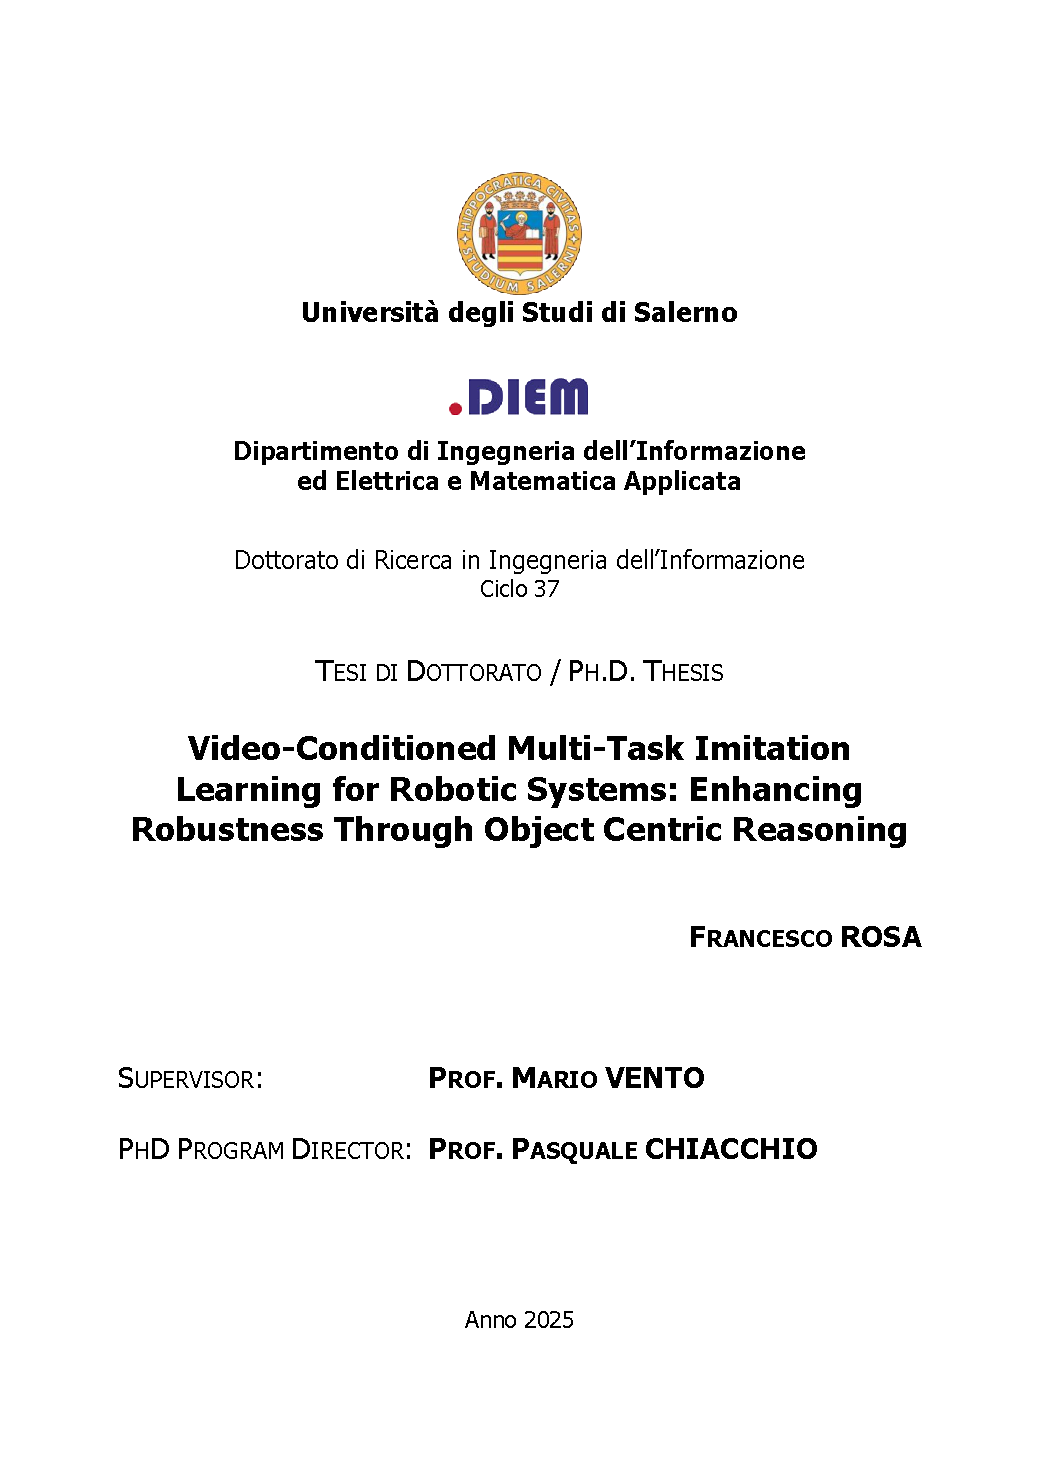
\includepdf{Frontespizio.pdf}


\chapter*{Abstract}
% 5 PAGINE E UN PO
\label{ch:abstract}
Robot technology is one of the pillars of modern society. Advances in information, electronic, and mechanical fields enable us to build and program machines to perform tasks in very different contexts, such as industry, surgery, and space missions.
\newline Specifically, in manufacturing, robots are mainly used to perform repetitive and unhealthy works like assembly, welding and material handling, thanks to their mechanical robustness and ability to repeatedly perform the same movements with high accuracy and precision.

While in the early day, robot systems were constrained in isolated and known environments. Over the past few decades, robots have been asked to solve tasks in dynamic and unknown/partially known environments, where they must \textbf{coexist} and \textbf{cooperate} with humans, while  solving different \textbf{dynamic} tasks \cite{bini2023multi} (e.g. pick a requested object, whose position is not known a priori). 

In this scenario, the desired characteristics of such robotic systems are:
\begin{enumerate}[label=\textbf{(\alph*)}]
\item \textbf{Adaptability to new conditions}, i.e., the system must be able to easily adapt to dynamic changes in system and environmental conditions, performing \textit{``intelligent" behaviors} to handle these new scenarios and solve the desired task.
\item \textbf{Adaptability to new tasks}, i.e., the system must be able to easily adapt to both new variations of a known task and completely new tasks by exploiting experience to infer actions and solve them.
% \item \textbf{Reliability}, i.e., the proposed system must be reliable in terms of success rate (tasks must be solved with a success rate that is reasonable for a real-world application), and safety (actions must not harm the environment, people, or the robot itself);
% \item \textbf{Computational efficiency}, i.e., the system must meet all the constraints above and run in real-time on real-world robot platforms as efficiently as possible.
\end{enumerate}

These requirements, can be challenging to achieve with traditional robot programming techniques based on hand-written policies and control methods. These conventional techniques often require a meticulous analysis of process dynamics, the construction of an analytical model, and the derivation of a control law that meets specific design criteria. This design process is tedious and time-consuming, particularly when high-level perception systems (e.g., cameras, microphones, motion sensors) are used to infer the state of the environment (such as the unknown position of a desired object relative to the end-effector) and the intentions of the human operator.

% In questo caso la funzione di controllo viene appresa dai dati, nello specifico, nel primo caso 
In contrast, significant advancements have been made by leveraging \textit{learning techniques}, where the control policy is inferred from data. This data can be generated either by \textbf{agent experience} \cite{sutton2018reinforcement} or by \textbf{expert demonstrations} \cite{osa2018algorithmic}. 
\newline In the case of agent experience, there is a trial-and-error procedure where the control policy generates actions executed by an agent, which interacts with the environment. The parameters are then tuned according to the effectiveness of the actions, based on their impact on the environment relative to the task to be solved. 
\newline In the case of expert demonstrations, the control policy parameters are directly tuned using a dataset containing examples of task execution. Here, the goal is to replicate the tasks observed in the dataset.

% In questo caso, la policy di controllo non è addestrata per eseguire un singolo task (pick an object), con l'obiettivo di generalizzare rispetto a diversi oggetti e diverse condizioni iniziali. Ma è addestrata per eseguire diverse variazioni di uno specifico task (e.g., pick an object with different possible placing location) o addirittura task  diversi tra di loro (e.g., una singola policy di controllo che risolve sia il problema del pick-place sia problemi di assemblaggio), con l'obiettivo di generalizzare rispetto agli oggetti che vengono manipolati, le condizioni iniziali e rispetto ai task stessi. Questo significa che, sfruttando l'ipotesi di knowledge-sharing possiamo ottenere un sistema in grado di risolvere nuove variazioni.  
Given this background, the thesis is framed in the context of \textit{Learning from Demonstration} (LfD), a learning approach based on expert demonstrations. According to the requirements of adaptability the thesis focus on a specific aspect of LfD, named \textit{Multi-Task LfD}. In this case, the control policy is not trained to execute a single task (e.g., picking an object) with the goal of generalizing across different objects and initial conditions \cite{zhang2018deep_vr_teleoperation,mandlekar2022matters}. Instead, it is trained to handle various variations of a specific task (e.g., picking an object from different possible locations) \cite{dasari2021transformers_one_shot} or even entirely different tasks (e.g., a single control policy that solves both picking and placing tasks as well as assembly tasks) \cite{brohan2022rt,mandi2022towards_more_generalizable_one_shot}. The goal is to generalize not only with respect to the objects being manipulated and the initial conditions but also with respect to the tasks themselves. This means that it is possible to achieve a system capable of solving new variations by leveraging the knowledge-sharing hypothesis.

In this scenario, the learning procedure is much more challenging because there is the need to include and define the \textbf{conditioning signal} (i.e., the signal that informs the policy about the task to execute, the object to manipulate, and the target placing location). Additionally, the environment can contain \textbf{multiple distractor objects} (e.g., objects that can potentially be manipulated but are not of interest for a given task variation). 

Regarding the conditioning signal, there are at least two intuitive approaches. The first is through a natural language description of the task to be executed \cite{stepputtis2020language,mees2022calvin,brohan2022rt}, and the second is through a video demonstration \cite{dasari2021transformers_one_shot,mandi2022towards_more_generalizable_one_shot}. 
\newline In the former, the task is described using phrases that specify the task details, such as ``Pick the red box and place it into the first bin". Given in input the phrase, the system must be able to infer the intent of the task (i.e., the pick-place operation) and the object of interest (e.g., red-box for picking and first bin for placing), and correlate this information with the environment and robot state to effectively control the robot.
\newline In the latter, another agent (either a robot or a human operator) performs the task in a different environment configuration, records this execution, and provides the video as input to the control policy. The control policy must then infer the intent from the video (i.e., the task to be performed, the object to be manipulated, and the final state) and control the robot to complete the task according to the agent's state, the environment's state, and the commanded task.

Inspired by how humans can learn to replicate tasks by simply observing their execution, the main goal of this thesis is to develop a system capable of replicating tasks shown in a video demonstration. This involves addressing challenges related to extracting task-relevant information from the video, such as identifying the manipulated object and its final position.

% Per quanto riguarda il problema legato alla presenza degli oggetti distrattori, in generale questi sono oggetti che non vengono mai considerati in operazioni di manipolazione, semplificando di molto il problema. Però nel contesto proposto in questa tesi il problema è ulteriormente enfatizzato dal fatto che il significato semantico di oggetto di interesse o distrattore associato agli oggetti presenti nella scena è definito a run-time dal comando stesso. Questo significa che se la configurazione iniziale è composta da 4 oggetti (e.g., 4 box di colore diverso), sulla base del comando dato al robot un determinato oggetto può diventare o meno di interesse. 
Regarding the issue of distractor objects, they are typically defined as items present in the scene but never involved in manipulation operations. Modern deep architectures can handle this scenario effectively, as they can easily learn to ignore these objects since they do not participate in any manipulation tasks. However, in the context proposed in this thesis, the problem is further complicated by the fact that the semantic meaning of an object (i.e., target or distractor) is defined at run-time by the command itself. This means that if the initial configuration consists of four objects (e.g., four boxes of different colors), a specific object may or may not be of interest based on the command given to the robot.

The primary contribution of this thesis is tackling the challenge of distractor objects. A key issue identified in existing literature is \textbf{target misidentification}, where the learned control policy generates valid trajectories, enabling the robot to reach, pick, and place objects, but frequently manipulates the wrong object.

To solve this problem, two main considerations were made:

\begin{enumerate}[label=\textbf{(\arabic*)}]
    \item Architectures proposed in the current literature are predominantly \textbf{end-to-end}, translating high-dimensional inputs, such as images, into corresponding low-dimensional actions. As a result, the model must learn an implicit representation that encodes both the task objective and the current state of the environment, including the location of the target object.
    \item The learning procedure optimizes an \textbf{action-centric \\ metric}, meaning that it is not directly linked to task success but instead focuses on mimicking the expert's actions on average. This action-focused optimization can lead to poor encoding of critical information, such as object positions.
\end{enumerate}

These two factors can result in a control policy that fails to effectively guide the robot toward the target object. In particular, it was observed that the early stages of trajectory execution are critical. Even small errors during these initial steps can cause the robot to reach and ultimately pick the wrong object.

Based on these considerations, this thesis explores the development of a \textbf{modular} architecture instead of an end-to-end approach \cite{foggia2024enhancing,foggia2024improving}. This architecture features modules specifically designed for reasoning about the objects of interest (e.g., target object and placement location). The outputs of these reasoning modules are then integrated to simplify the learning problem for the Control Module. This module is now informed by low-dimensional information, such as the position of the target object, which may be more effectively utilized during the learning process, especially in light of the action-centric cloning loss.

To perform this explicit reasoning, a \textit{Conditioned Object Detector} (COD) has been developed. This module, given the video demonstration and the current agent observation as input, predicts the category-agnostic bounding box related to the target object and the final placing location. This low-level positional information is then provided to the control module, which predicts the actions to perform.

The learning procedure is then divided into two steps. The first step involves training the COD module, which focuses on explicitly solving cognitive tasks, such as detecting regions of interest represented by the object to be manipulated and its final location. The second step involves training the \textit{Object Conditioned Control Policy} (OCCP), which focuses on solving the control problem using low-level positional information that can be easily mapped into the corresponding actions.

The final system has been extensively tested in simulation environments, then it was also validated on a real-world robotic platform. 

Regarding the simulated environment, the system was evaluated on both \textbf{multi-variation single-task} scenarios and \\ \textbf{multi-variation multi-tasks} scenarios, considering four simulated tasks: Pick-Place, Nut-Assembly, Stack-Block, and \\ Button-Press. Each task had different variations based on the manipulated object and the final state. While the tasks share common properties, they also have specific characteristics. For example, the Nut-Assembly task involves contact-rich, precise manipulation, whereas Pick-Place can be solved in a much rougher manner.

Overall, the proposed methods demonstrated very promising behaviors and a general improvement over baseline methods that do not include object-related reasoning. Specifically, in the single-task multi-variation scenarios, the proposed method achieved a success rate of \textbf{90.13\%} on average, which is an improvement of \textbf{+28.78\%} compared to the baseline method. In the multi-task multi-variation scenarios, the proposed method achieved a success rate of \textbf{79.24\%} on average, which is an improvement of \textbf{+33.23\%} compared to the baseline method.
This shows that solving manipulation tasks with an object-oriented approach can be an effective paradigm for LfD problems. Additionally, this approach provides interpretable information to the end user, as the predicted bounding boxes can be interpreted as the locations where the robot will move.

In conclusion, the proposed method was tested also in a real-world environment, where the complexity of the problem is heightened by the presence of less and noisy data collected through teleoperation. Even under these challenging conditions, the proposed method demonstrated its effectiveness in addressing both the cognitive and control problems, reaching a success rate of \textbf{55.00\%}, which is a strong improvement with respect to the \textbf{0.00\%} of the baseline method in the same training condition. This confirms that the object prior can be successfully applied in real-world scenarios, enabling the development of a reliable system despite limited and noisy trajectory data.


\tableofcontents       % Inserisce l'indice della Tesi

\clearemptydoublepage
\thispagestyle{empty}

\begin{flushright}
	\null\vspace{\stretch{1}}

	\emph{Will robots inherit the earth? Yes, but they will be our children.}

	\emph{}

	- Marvin Lee Minsky -

	\vspace{\stretch{5}}\null
\end{flushright}

\pagestyle{fancy} % Abilita lo stile Fancy per le pagine

%\include{Acknowledgment} % Togliere commento per inserire i ringraziamenti (file esterno Ringraziamenti.tex)


% --- Definisce gli header per le pagine pari e dispari ---
\renewcommand{\sectionmark}[1]{\markright{\thesection.\ #1}}
%\renewcommand{\chaptermark}[1]{\markboth{\MakeUppercase{\chaptername\ \thechapter.\ #1}}{}}
\renewcommand{\chaptermark}[1]{\markboth{\thechapter.\ #1}{}}

\fancyhf{}

\fancyhead[LE,RO]{\footnotesize \slshape \bfseries \thepage}
\fancyhead[LO]{\footnotesize \slshape \bfseries \rightmark}
\fancyhead[RE]{\footnotesize \slshape \bfseries \leftmark}
\fancypagestyle{plain}{\fancyhead{} \renewcommand{\headrulewidth}{0pt}}

\renewcommand{\headrulewidth}{0.5pt}
\renewcommand{\footrulewidth}{0pt}
\addtolength{\headheight}{0.5pt}

% --- Fine definizione header


\pagenumbering{arabic} % Definisce il nuovo stile di numerazione delle pagine

% THEOREMS ----  Si ridefiniscono gli stili dei teor., lemmi corollari
\theoremstyle{plain}
\newtheorem{thm}{Theorem}[section]
\newtheorem{cor}[thm]{Corollary}
\newtheorem{lem}[thm]{Lemma}
\newtheorem{prop}[thm]{Proposition}
%
\theoremstyle{definition}
\newtheorem{defn}{Definition}[section]
%
\theoremstyle{remark}
\newtheorem{rem}{Remark}[section]


% Thesis chapters -------------------------------------------------------
% Ogni capitolo è scritto in un file .tex da includere.
% Tali file devono cominciare con il comando \chapter{}
% I file di Introduzione e Conclusione possono cominciare con \chapter*{}

%\addcontentsline{toc}{chapter}{Introduction}
%\thispagestyle{empty}

%\thispagestyle{empty}


%\addcontentsline{toc}{chapter}{State of the Art}
%\include{StateArt}
%\thispagestyle{empty}

%% Add content
\chapter{Introduction}
% \subsection{Application Context}
\section{Motivation and thesis overview}
\section{Learning from Demonstrations}
\label{sec:sota}
The chapter provides a comprehensive review of LfD problem, offering an overview of the problem itself and the progression of methodologies developed to address it over time. Specifically, Section~\ref{sec:problem_formulation} will focus on the formal definition of the LfD problem. Following that, Section~\ref{sec:lfd} will discuss various approaches and methodologies used to solve the problem. This section will include a detailed taxonomy of these approaches, highlighting their respective advantages and disadvantages, and concluding with considerations that are relevant to the objectives of this thesis.
\subsection{Problem formulation}
\label{sec:problem_formulation}
\subsection{Learning from demonstration}
\label{sec:lfd}
This section is dedicated to presenting and analyzing various approaches for solving the LfD problem described in Section~\ref{sec:problem_formulation}. Specifically, this section follows the taxonomy derived from studying different review papers~\cite{kaelbling1996reinforcement_survey,argall2009robot_learning_from_demonstration,hussein2017imitation_learning_survey,fang2019survey,zheng2021imitation_progress_taxonomies_opportunities,zare2024survey}. Figure~\ref{fig:il_taxonomy} provides a graphical representation of the proposed taxonomy. The methods are first categorized based on the type of demonstration, either \textit{State-Action} or \textit{State-only}, followed by an overview of the different methodologies. The proposed taxonomy highlights the learning algorithm and main components for each methodology.

This chapter is divided into the following sections. Section~\ref{sec:bc} reviews methods for the fully-supervised learning methodology known as Behavioral Cloning. 
\newline Section~\ref{sec:irl} discusses methods under the umbrella of Inverse Reinforcement Learning, which solve the inverse optimization problem by first learning the reward function and then using it to guide policy optimization following a reinforcement paradigm
\newline Section~\ref{sec:gail} reviews methods leveraging the concept of \textit{Generative Adversarial Learning} to optimize policy parameters and learn demonstrated behaviors, classified as Generative Adversarial Imitation Learning methods.
\newline Finally, Section~\ref{sec:lfo} covers the most recent methodology, Learning from Observation, characterized by optimizing the learner policy using state-only demonstrations.
\input{figures/ch1/taxonomy.tex}
Each paragraph will present the research in the same way, i.e., the proposed works will be presented in a temporal order, highlighting the evolution of techniques and approaches over time.
It is important to note that with respect to the problem managed in this thesis, the most relevant and most related literature is the one preseneted in Section \ref{sec:bc}. However, for sake of clarity and completeness, all the other approaches will be described with their pros/cons, with some considerations with respect to the proposal of this thesis. \todo{ADD THIS DISCUSSION}.


\input{chapters/ch1/sota/bc.tex}
\input{chapters/ch1/sota/irl.tex}
\input{chapters/ch1/sota/gail.tex}
\input{chapters/ch1/sota/lfo}





% \subsection{Graph Neural Network for planning systems}
\label{sec:gnn_planning}
\chapter{Proposed conditioned object detector}
\label{ch:cod}
As discussed in Section \ref{sec:motivation}, this thesis proposes a modular approach to solve the Visual-Conditioned Multi-Task Imitation Learning Problem. This chapter focuses on the module responsible for addressing an instance of the ``Cognitive Task" relevant to the context under consideration. Specifically, the approach aims to leverage an \textbf{object-prior} to enable the system to ignore distractor objects in the scene and focus on the target region of interest. To achieve this goal, a preliminary step is to develop a system capable of computing this object-prior. Therefore, this chapter will present and discuss the design of the Conditioned Object Detector (COD), which is specifically designed to solve a \textbf{novel variation} of the well-known Object Detection problem. Unlike traditional object detection tasks, where a deep architecture produces bounding boxes for all objects in the scene, this variation requires generating bounding boxes only for the regions of interest based on the demonstrated task.

Section \ref{sec:cod_related_works} will review relevant methods related to this task. 
Section~\ref{sec:cod_problem} outlines the detection problem being addressed. Section~\ref{sec:cod_architecture} describes the proposed architecture for solving this problem. Finally, Section~\ref{sec:cod_experimental} discusses the experimental setup and presents the results obtained from testing the proposed architecture.

\section{Related Works}
\label{sec:cod_related_works}
This section will review the preliminary research conducted in the context of Object-Oriented Imitation Learning (Section \ref{sec:ooil}) to understand how previous studies have leveraged object priors to solve the Learning from Demonstration (LfD) problem. Additionally, it will examine research in the context of Visual-Question Answering (Section \ref{sec:vqa}) to highlight the specific challenges addressed by the COD module, while also presenting the methods that have primarily inspired the proposed solution.

\subsection{Object-Oriented Imitation Learning}
\label{sec:ooil}
All the methods discussed in Section \ref{sec:lfd} share a common characteristic: they are end-to-end systems that take high-level inputs, such as images, and directly generate the corresponding actions as output. While this approach can be sufficient in scenarios where the scene is simple, meaning there are no distracting objects, or if there are distracting objects, they can be easily identified by the system because they are consistently not involved in the manipulation, this end-to-end approach may struggle in more complex environments. Specifically, it can encounter difficulties when the robot workspace contains objects that are similar to each other, especially if these objects are involved in manipulation for some task variations.

Based on this consideration, this paragraph will describe methods that leverage object priors. This means that the control policy is informed not only by the embedding of the agent scene, which is obtained from a deep architecture, but also by object-level information, such as the bounding boxes of objects in the scene, obtained from an object detector.

The concept of leveraging object priors has been explored in both earlier works \cite{devin2018deep,park2021object} and more recent approaches \cite{belkhale2023plato,zhu2023viola,zhu2023learning,jiang2023vima}.

One of the preliminary works on leveraging object priors was presented by the authors of \cite{devin2018deep}. This work primarily focuses on the challenge of generalization in Learning from Demonstration (LfD) systems that use an end-to-end approach. In such systems, a task-specific model is trained to predict actions based on raw visual observations. The authors found that while it is possible to achieve good \textit{instance-level generalization}, meaning the model can solve tasks with varying initial configurations using a limited number of samples, achieving \textit{category-level generalization} is more challenging. Category-level generalization refers to the model ability to solve tasks involving different objects. To achieve this, the dataset must include a large number of trajectories involving a wide variety of objects. For instance, if the task is to pour the contents of a bottle into a cup, the dataset should contain trajectories with different types of cups and bottles. However, constructing such a dataset is time-consuming and costly. Moreover, the potential of well-known large datasets in classical computer vision tasks, such as object detection, is not fully utilized.

To address this issue, the authors proposed a paradigm shift by introducing a robotic vision framework that operates on sets of objects rather than raw pixel data. This framework leverages prior datasets to learn a generic object concept model, thereby enhancing category-level generalization without requiring an extensive and diverse dataset. The framework is illustrated in Figure \ref{fig:object_prior_framework} and is composed of several stages:
\begin{itemize}
    \item \textbf{Meta-Attention}, which is basically a Region Proposal Network (RPN) \cite{fastrcnn}, trained on the well known MSCOCO \cite{lin2014microsoft} dataset. The RPN generates objects proposals, i.e., region of the image that possibly contain an object.
    \item \textbf{Task-Specific Attention}, which aims to learn what are the object of interest with respect to the task in hand. This module is parameterized as a vector $w$ such that the attention paid to $o^i$ is proportional to $e^{w^Tf(o^i)}$.
    \item \textbf{Soft Attention}, this module gives a probabilistic meaning to the attention map obtained from the Task-Specific Attention. Specifically, a Boltzmann distribution is used to map the attention weights to a probability for each object proposal, i.e., $p\left(o^i \mid w_j\right)=\frac{e^{w_j^{\top} \frac{f\left(o^i\right)}{\left\|f\left(o^i\right)\right\|_2}}}{\sum_{i=0}^N e^{w_j^{\top} \frac{f\left(o^i\right)}{\left\|f\left(o^i\right)\right\|_2}}}$.
    \item \textbf{Movement Prediction Network}, this module predicts the next robot action, given the attended object information from the soft attention, and the robot state represented by the joint and end-effector state.
\end{itemize}
\input{figures/ch1/object_prior_framework.tex}
This preliminary work focused mainly on two tasks:
\begin{itemize}
    \item  \textit{Pouring Task}: The robot is required to pour contents from a bottle into a mug. The challenge is to locate the mug from an image without being explicitly provided its location, especially when different mugs are used during training and testing.
    \item \textit{Sweeping Task}: The robot must sweep an object (e.g., a plastic orange) into a dustpan, with both objects starting in different positions. This task requires the robot to adapt its approach based on the relative positions of the objects.
\end{itemize}
During testing, the authors focused on \textit{Category Generalization} and the ability to \textit{Ignore Distractor Objects}. For the former, the system was trained with only one type of mug and evaluated with other mugs (Figure \ref{fig:pouring_task_setting}). The results showed that the system successfully poured the contents into the correct mug, thanks to the learned task-specific attention weight that highlighted the mug features. For the latter, the authors designed a test where two mugs were present in the scene (Figure \ref{fig:task_specific_attention}). Since the model did not receive any conditioning signal indicating which mug to use, the authors fine-tuned the attention weight on trajectories where only the brown mug was used, demonstrating that this mechanism could focus on more specific features, such as the mug color.
\input{figures/ch1/object_prior_framework_task.tex}

In summary, this preliminary work demonstrated that leveraging object priors can facilitate category-level generalization by utilizing large, well-known datasets for the object-detection problem. However, the experimental setup was relatively simple, even in scenarios with distractor objects. The proposed system could handle distractor objects only after specific fine-tuning and was not able to dynamically discriminate between objects of interest and distractors based on task variations.

A recent work that follows a similar approach is proposed in \cite{zhu2023viola}. In this work, the authors introduced VIOLA (Visuomotor Imitation via Object-centric Learning) (Figure \ref{fig:viola_architecture}), an architecture inspired by the ideas presented in \cite{devin2018deep}. VIOLA uses an RPN and a ResNet18 \cite{resnet} to generate object proposals and produce a spatial feature map, respectively. It then constructs a \textit{per-step feature} vector, composed of three key elements: a \textbf{global context feature} that encodes the current task stage, an \textbf{eye-in-hand visual feature} to mitigate occlusion, and a \textbf{proprioceptive feature} that captures the robot state. These per-step features are concatenated to form a \textbf{history of observations}, which is designed to capture temporal dependencies and dynamic changes in object states. This tensor is then fed into a Transformer \cite{vaswani2017attention}, which leverages its intrinsic attention mechanism to automatically focus on the object of interest.
\input{figures/ch1/viola_architecture.tex}
This method was first evaluated in a simulation environment across three tasks, as depicted in Figure \ref{fig:viola_task}. Various testing scenarios were considered, including different object placements, the introduction of distractor objects, and changes in camera position. Generally speaking, VIOLA outperformed all baselines across these testing conditions, further demonstrating the utility of object priors in enhancing the robustness of such methods. However, similar to \cite{devin2018deep}, the testing scenarios were relatively simple, with clear distinctions between distractors and objects of interest. The distractors were objects never seen during the demonstration and were not involved in manipulation, making them relatively easy for the model to discriminate.

In the works discussed so far, the approach has primarily focused on leveraging object priors to directly predict the actions that the robot must perform. However, a different approach was proposed in \cite{belkhale2023plato}, where the authors introduced an alternative interpretation of object-centric concept. Instead of focusing on the robot perspective, they shifted the emphasis to the object perspective, proposing PLATO (Predicting Latent Affordances Through Object-Centric Play). PLATO is a learning framework that learns a \textbf{latent affordance space}, which describes how an object can be used (e.g., a block being grasped, a door knob being turned, or a drawer being opened).

The authors argue that learning these affordances (i.e., what happens to the object) rather than plans (i.e., what happens to the robot) from play leads to a simpler and more robust task representation that can operate over varying time horizons. This, in turn, results in more effective policies at test time. This paradigm shift allows the policy to reason about the environment more effectively: given access to an affordance (e.g., the door knob being turned) and a goal (e.g., an opened door), the policy can work backwards to infer the behavior needed to exploit that affordance (e.g., reaching the knob and rotating the gripper to turn it).

To reach this objective authors started from the observation that a single-object manipulation is composed of the following three phases:
\begin{enumerate}
    \item \textbf{Pre-interaction}, when the robot prepares to interact with an object (e.g., reaching for a block).
    \item \textbf{Interaction}, when the robot and the object engage in joint actions (e.g., pushing or pulling the block).
    \item \textbf{Post-interaction}, when the robot separates from the object, and the object may come to rest (e.g., the block stops moving).
\end{enumerate}
Given these three phases, the algorithm learns a \textbf{latent affordance distribution}. Specifically, the architecture comprises three learnable modules:  $E$,  $E'$, and  $\pi$.  $E$ models the posterior distribution, mapping the full interaction trajectory  $\tau^{i}$ to the corresponding latent affordance distribution, from which the affordance embedding  $z$ is sampled.  $E'$ is the prior module used during rollout. It takes the current state and the goal state as input and generates the affordance embedding  $z'$. This module is trained to match the posterior distribution modeled by  $E$.  $\pi$ represents the current policy, which generates the action  $a^{i}$ given the current state  $s^{i}$, the desired goal  $o_g$, and the latent embedding  $z$.

These three modules are trained end-to-end by minimizing the loss function in Formula \ref{eq:plato_equation}, which includes three terms. The first two terms correspond to the policy  $\pi$, ensuring it matches the ground-truth trajectories in the interaction and pre-interaction phases. The last term is the KL-divergence, used to train the posterior and prior modules  $E$ and  $E'$.

\begin{equation}
    \label{eq:plato_equation}
    \begin{aligned}
        \mathcal{L}_{PLATO} = -\log \left(\pi\left(a_{1: H}^{(i)} \mid s_{1: H}^{(i)}, o_g, z\right)\right)- \\ 
        \alpha \log \left(\pi\left(a_{1: H}^{(-)} \mid s_{1: H}^{(-)}, o_g, z\right)\right)+ \\ 
        \beta \operatorname{KL}\left(p(z) \| p\left(z^{\prime}\right)\right)
    \end{aligned}
\end{equation}
\input{figures/ch1/plato.tex}

Finally, this method was tested in a variety of scenarios, including both single-object and multiple-object manipulation with different manipulation primitives (Figure \ref{fig:plato_task}). However, in the multi-object scenarios, the system was only tested on single-object manipulation primitives.

This work is particularly noteworthy as it demonstrates that a policy can be learned by solving an inverse problem, starting from object affordances and deriving the corresponding robot trajectories. It also shows that the policy can be conditioned based on the desired goal state. However, certain aspects were not addressed in this work, such as the potential presence of distractor objects and tasks requiring the manipulation of multiple objects. Additionally, the affordances were learned in the object space (i.e., with known object poses) rather than in the high-level image space.

The works discussed in this paragraph highlight the significant research efforts aimed at modeling the manipulation problem from an object-centric perspective. These efforts either focus on the affordances of the object (i.e., the possible movements the object allows) or introduce object priors defined by regions of interest that may contain the object to be manipulated, with results demonstrated in both simulated and real-world environments. However, the methods presented so far primarily address single-task scenarios, where distractor objects can be easily identified as they remain constant across demonstrations. In contrast, this thesis proposes a solution for a more challenging scenario in which the robot operates in a multi-variation environment. This environment includes multiple similar objects, which may serve as either targets or distractors depending on the specific task variation.

\subsection{Visual-Question Answering}
\label{sec:vqa}
The \textit{Visual-Question Answering} (VQA) problem refers to the ability of a system of ``reasoning'' over an image, based on a given query expressed in terms of text. This means that, given in input an arbitrary image and an arbitrary textual prompt the system must be able to generate an answer to the given prompt (Figure \ref{fig:vqa_example}).
\input{figures/ch2/vqa_problem.tex}

The key aspect related to this problem is related to the fact that for a given image different questions can be made. There is no predefined mapping between an input image and its corresponding answer. Instead, the system must dynamically adjust its \textbf{attention} to specific regions of the image based on the given query. This requires effectively \textbf{correlating} the image encoding with the prompt encoding to generate a conditioned embedding that can reliably produce a valid answer.

Based on these preliminary considerations, various solutions have been proposed using both Convolutional Neural Network architectures \cite{perez2018film} and novel Transformer architectures \cite{chen2022caan,chen2024mpcct,liu2024visual}.

A significant breakthrough in this field was introduced in \cite{perez2018film}, where the FiLM (Feature-wise Linear Modulation) conditioning layer was proposed. The core idea behind FiLM is to dynamically modify the output of a neural network by applying an affine transformation to its intermediate features based on some input. Specifically, the FiLM layer learns two functions, $f$ and $h$, which produce the coefficients $\gamma_{i,c}$ and $\beta_{i,c}$, respectively, based on an input $x_{i}$, as defined in Equation \ref{eq:film}.
\begin{equation}
    \label{eq:film}
    \begin{matrix}
        \gamma_{i,c} = f_{c}(x_{i}) & 
        \beta_{i,c} = h_{c}(x_{i})
    \end{matrix}
\end{equation}
These coefficients are then used to modulate the $c^{th}$ activation map $\textbf{F}_{i,c}$ through a \textit{feature-wise affine transformation}, as described in Equation \ref{eq:film_eq}.
\begin{equation}
    \label{eq:film_eq}
    FiLM(\textbf{F}_{c}|\gamma_{c}, \beta_{c}) = \gamma_{c} \textbf{F}_{c} + \beta_{c}
\end{equation}

An example of integrating the FiLM layer into a deep architecture is shown in Figure \ref{fig:film_architecture}, illustrating the implementation proposed in \cite{perez2018film}. In this configuration, the prompt is encoded using a Gated Recurrent Unit (GRU), and the resulting embedding is fed into a Multi-Layer Perceptron (MLP), which outputs the coefficients $\gamma_{i,c}$ and $\beta_{i,c}$. These coefficients are subsequently used to modulate the activations of $N$ Residual Blocks (ResBlocks).
\input{figures/ch2/film_integration.tex}

The FiLM layer has also been effectively applied in the context of Language-Conditioned Policy Learning (Section \ref{sec:occp_mtil}) \cite{jang2022bc_z,brohan2022rt}. Starting from a textual prompt describing a desired task, the FiLM layer modulates the activation maps of the convolutional blocks in the network that encodes the robot's observations. This allows the network to focus on specific parts of the image relevant to the task (Figure \ref{fig:film_attention}).
\input{figures/ch2/film_attention_mechanism.tex}

Since the introduction and expansion of Transformer models \cite{vaswani2017attention}, there has been a major shift towards solving the Visual Question Answering (VQA) problem by utilizing these architectures. Transformers excel at capturing intra-modal relationships through dependency modeling and promoting alignment and interaction between multiple modalities. This has led to the development of Vision-Language Transformers capable of directly processing multi-modal inputs, such as images and text. An example is the LLaVA model proposed in \cite{liu2024visual}, which represents the current state-of-the-art in VQA. However, despite its capability to handle complex queries, LLaVA relies on a Large Language Model (LLM) with a minimum size of 7 billion parameters, requiring a high-performance server. This makes real-time deployment in real-world systems, such as robotic control, challenging or even impractical.


\section{Problem formulation}
\label{sec:cod_problem}
\section{Architecture}
\label{sec:cod_architecture}
\section{Experiments}
\label{sec:cod_experimental}
In this section, the performed experiments are going to be described. Specifically, in  
Section~\ref{sec:cod_dataset} the dataset used for training procedure will be described. Section~\ref{sec:cod_results} will report the obtained results.
\subsection{Dataset}
\label{sec:cod_dataset}
To validate the proposed architecture, a simulated dataset was generated, focusing on four primary tasks: \textit{Pick-Place}, \textit{Nut-Assembly}, \textit{Stack-Block}, and \textit{Press-Button}. Each task consists of multiple variations. Specifically, the Pick-Place task has 16 variations, Nut-Assembly has 9 variations, Stack-Block has 6 variations, and Press-Button has 6 variations. Each task and its variations are graphically described in Figure~\ref{fig:dataset_cod}.
\begin{figure}[t]
    \centering
    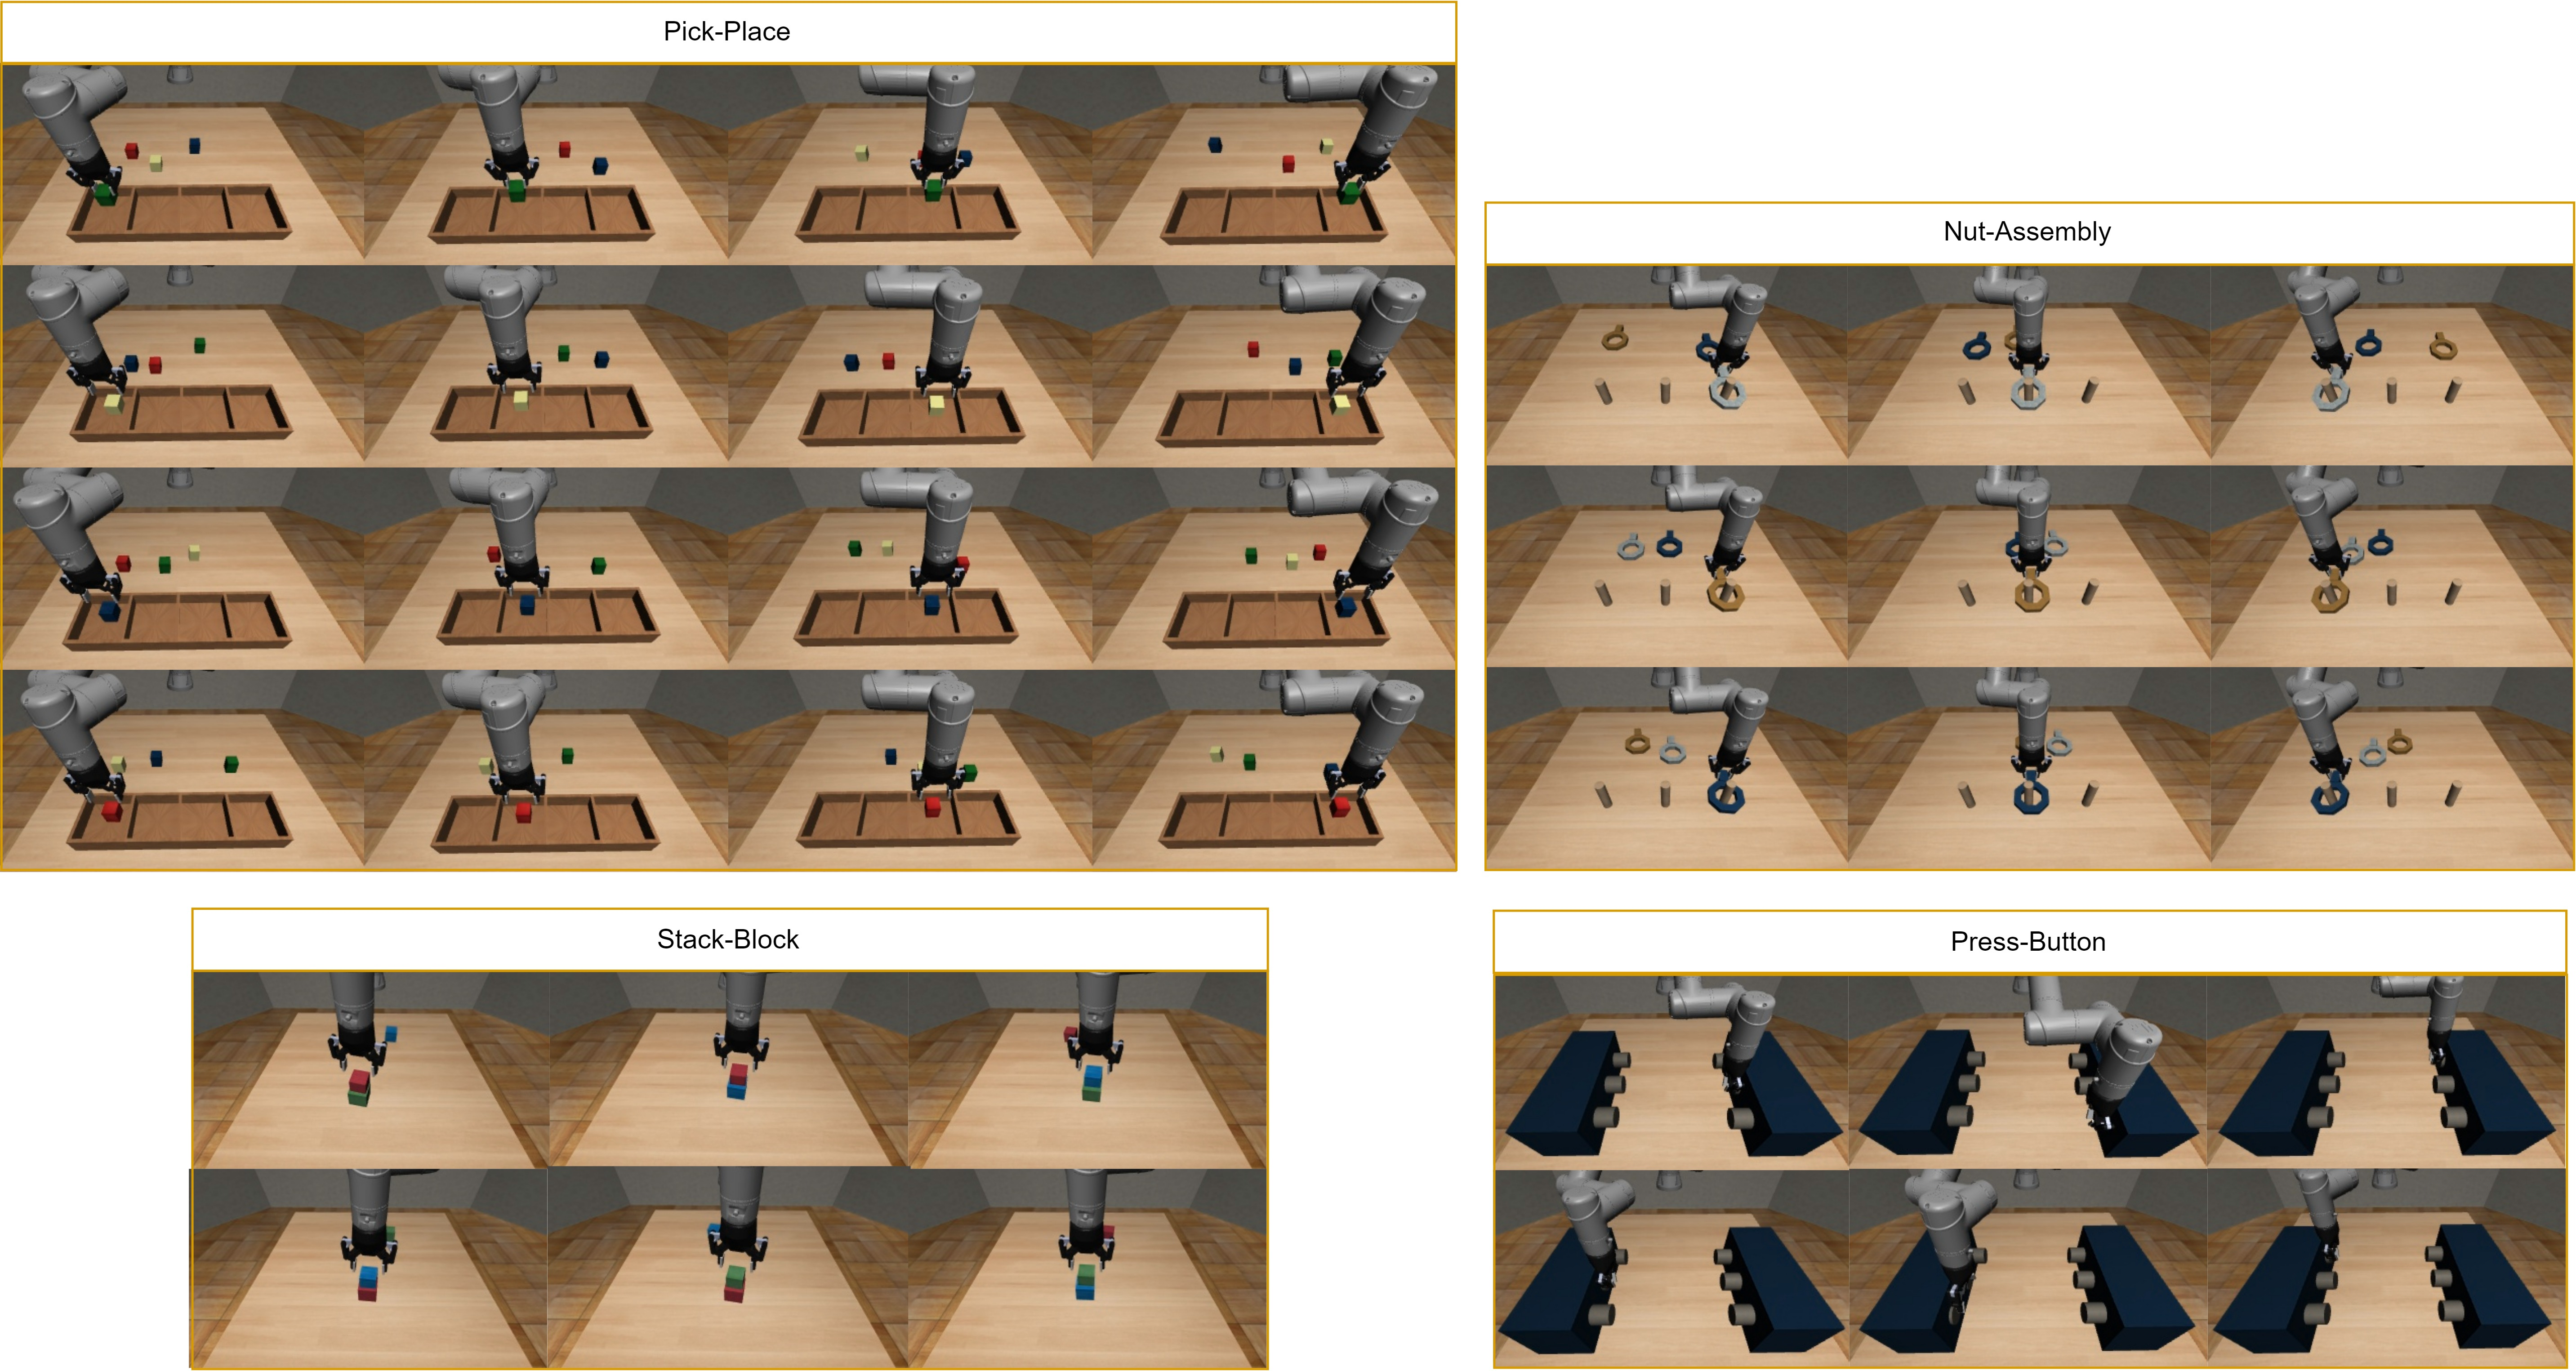
\includegraphics[width=1.0\textwidth]{figures/images/ch2/dataset.jpg}
    \caption{Examples of tasks and variations taken in consideration for the methods validation. The images report the final system state. For the pick-place, nut-assembly and stack-block tasks the variation is defined with respect to the target object and the placing location, while for the press-button the variation is defined according to the button to press.}
    \label{fig:dataset_cod}
\end{figure}


For each task, 100 trajectories were collected for both the agent (UR5e robot) and the demonstrator (Franka-Emika Panda robot) using hand-written policies that take as input ground-truth information about the object position. Across these trajectories, the position of the objects of interest varies. The workspace for each task is divided as follows:
\begin{itemize}
    \item \textbf{Pick-Place}: The bins are fixed in position, while the boxes can change according to the following rule. The workspace is divided into 4 slots, parrallel to the bins, each with a width of $6 \ \text{cm}$ and a height of $15 \ \text{cm}$. A slot is randomly selected, and the box is randomly spawned within the chosen slot, ensuring that each slot is filled with only one object.
    \item \textbf{Nut-Assembly}: The pegs are fixed in position, while the nuts vary in placement. A spawn region of $75 \times 10 \ \text{cm}$ is defined, and the nuts are randomly spawned in this region, ensuring they do not collide with one another.
    \item \textbf{Stack-Block}: The placing box is spawned in a region of $16 \times 5 \ \text{cm}$, while the target box is spawned in a region of $24 \times 5 \ \text{cm}$, ensuring no collisions between the boxes.
    \item \textbf{Press-Button}: The two sets of buttons are placed within a region of $4 \times 4 \ \text{cm}$.
\end{itemize}

The bounding-boxes are automatically generated. The procedure followed to generate the bounding boxes assume the knowledge of the pose and dimention of the object, as well as the knowledge of the pose of the camera and its intrinsic parameters. Giving all these information, it is possible to build a 3D bounding-box around the object in the continous world space, then project the corners in the 2D discrete camera space through a sequence of transformations described in Formula \ref{}.
\begin{equation}
\end{equation}
\smalltodo{add equation}
\subsection{Results}
\label{sec:cod_results}
This section presents the obtained results, divided into two main blocks. The first block (Section~\ref{sec:cod_tod}) discusses the results of the method trained to detect only the target object. The second block (Section~\ref{sec:cod_tod}) covers the results of the method trained to detect both the target object and the final (placing) location. For each method, results are reported for two different scenarios: first, where the method is trained in a single-task multi-variation scenario; and second, where the method is trained in a multi-task multi-variation scenario.

For all the test configurations described below, the testing procedure was consistent. Specifically, for each task and its variations, 10 rollouts were performed. During each rollout, the robot was controlled by a hand-written policy, and the predicted bounding box was compared with the ground truth, obtained using the same procedure as described earlier.

The metrics used to evaluate the methods were \textit{Precision@0.5} (Equation \ref{eq:prec}) and \textit{Recall@0.5} (Equation \ref{eq:rec}).
\begin{equation}
    \label{eq:prec}
    Pre = \frac{TP}{TP+FP}
\end{equation} 
\begin{equation}
    \label{eq:rec}
    Rec = \frac{TP}{TP+FN}
\end{equation}

A \textit{True Positive} (TP) sample is defined as a predicted bounding box for the target class with an Intersection over Union (IoU) greater than or equal to 0.5 when compared with the ground-truth bounding box. A \textit{False Positive} (FP) sample is defined as a predicted bounding box for the target class with an IoU less than 0.5. A \textit{False Negative} (FN) sample is defined as a target object for which no bounding box was predicted.

The metrics were computed considering only the target bounding boxes, i.e., the bounding boxes predicted for the target object or the target location. Among all the candidates generated by the network, only the one with the highest predicted class score was considered.


\subsubsection{Target object detector}
This first set of validation tests is related to the training of the COD module in a setting where it must predict the location of the target-object. This means that, with respect to the semantic attributes defined in Section \ref{sec:cod_problem}, the set is restricted to just two classes ``target'' and ``no-target''. In this case, the method will be named \textit{Conditioned Target Object Detector} (CTOD).
\label{sec:cod_tod}
\paragraph*{Single-task multi-variation scenario}\mbox{}\\
In the single-task multi-variation scenario, a specific model was trained for each task described in Figure \ref{fig:dataset_cod}. This approach allows for evaluating the model ability to handle tasks of increasing complexity. Initially, the model is evaluated in a simpler scenario, where it predicts the target position of a specific category of objects (e.g., only boxes in pick-and-place, or only nuts in nut-assembly), thereby limiting variability in object categories.
% \usepackage{graphicx}
% \usepackage{hhline}

% \usepackage{hhline}


% \usepackage{graphicx}
% \usepackage{hhline}


\begin{table}[t]
    \centering
    \caption{Results of the CTOD module obtained in the single-task multi-variation scenario. Performances are reported in terms of \textit{Precision} (Prec), \textit{Recall} (Rec) with an IoU threshold of 0.5 and the Average IoU $(IoU_{avg})$ }
    \label{table:ctod_single_task_performance}
    \begin{tabular}{|c|c|c|c|} 
    \hline
    \textbf{Task} & \textbf{Precision@0.5} & \textbf{Recall@0.5} & $\mathbf{IoU_{avg}}$ \\ 
    \hhline{|====|}
    Pick-Place & 0.770 & 1.00 & 0.628 \\ 
    \hline
    Nut-Assembly & 0.985 & 1.00 & 0.789 \\ 
    \hline
    Stack-Block & 0.995 & 1.00 & 0.848 \\ 
    \hline
    Press-Button & 0.997 & 1.00 & 0.899 \\
    \hline
    \end{tabular}
    \end{table}

% \begin{table}[t]
%     \centering
%     \refstepcounter{table}
%     \caption{Distribution of the predicted bounding boxes generated by the CTOD module in the single-task, multi-variation scenario.}
%     \label{table:ctdo_single_task_prediction_distribution}
%     \resizebox{\linewidth}{!}{%
%     \begin{tabular}{|c|c|c|c|c|c|} 
%     \hline
%     \textbf{Task} & \textbf{TP} & \begin{tabular}[c]{@{}c@{}}\textbf{FP }\\\textbf{pre-picking}\end{tabular} & \begin{tabular}[c]{@{}c@{}}\textbf{FP }\\\textbf{post-picking}\end{tabular} & \begin{tabular}[c]{@{}c@{}}\textbf{FN }\\\textbf{pre-picking}\end{tabular} & \begin{tabular}[c]{@{}c@{}}\textbf{FN }\\\textbf{post-picking}\end{tabular} \\ 
%     \hhline{|======|}
%     \begin{tabular}[c]{@{}c@{}}Pick-Place \\(XXXX)\end{tabular} & XXXX & XXXX & XXXX & XXXX & XXXX \\ 
%     \hline
%     \begin{tabular}[c]{@{}c@{}}Nut-Assembly \\(XXXX)\end{tabular} & XXXX & XXXX & XXXX & XXXX & XXXX \\ 
%     \hline
%     \begin{tabular}[c]{@{}c@{}}Stack-Block\\(XXXX)\end{tabular} & XXXX & XXXX & XXXX & XXXX & XXXX \\ 
%     \hline
%     \begin{tabular}[c]{@{}c@{}}Press-Button\\(XXXX)\end{tabular} & XXXX & XXXX & XXXX & XXXX & XXXX \\
%     \hline
%     \end{tabular}
%     }
%     \end{table}

\begin{table}[t]
\centering
\caption{Results of the CTOD module obtained in the multi-task multi-variation scenario. Performances are reported in terms of \textit{Precision} (Prec), \textit{Recall} (Rec) with an IoU threshold of 0.5 and the Average IoU $(IoU_{avg})$}
\label{table:ctod_multi_task_performance}
\begin{tabular}{|c|c|c|c|} 
\hline
\textbf{Task} & \textbf{Precision@0.5} & \textbf{Recall@0.5} & $\mathbf{IoU_{avg}}$ \\ 
\hhline{|====|}
Pick-Place & 0.652 & 1.00 & 0.563 \\ 
\hline
Nut-Assembly & 0.948 & 1.00 & 0.726 \\ 
\hline
Stack-Block & 0.894 & 1.00 & 0.708 \\ 
\hline
Press-Button & 0.977 & 1.00 & 0.825 \\
\hline
\end{tabular}
\end{table}

% \begin{table}[t]
%     \centering
%     \refstepcounter{table}
%     \caption{Distribution of the predicted bounding boxes generated by the CTOD module in the multi-task, multi-variation scenario.}
%     \label{table:ctdo_multi_task_prediction_distribution}
%     \resizebox{\linewidth}{!}{%
%     \begin{tabular}{|c|c|c|c|c|c|} 
%     \hline
%     \textbf{Task} & \textbf{TP} & \begin{tabular}[c]{@{}c@{}}\textbf{FP }\\\textbf{pre-picking}\end{tabular} & \begin{tabular}[c]{@{}c@{}}\textbf{FP }\\\textbf{post-picking}\end{tabular} & \begin{tabular}[c]{@{}c@{}}\textbf{FN }\\\textbf{pre-picking}\end{tabular} & \begin{tabular}[c]{@{}c@{}}\textbf{FN }\\\textbf{post-picking}\end{tabular} \\ 
%     \hhline{|======|}
%     \begin{tabular}[c]{@{}c@{}}Pick-Place \\(XXXX)\end{tabular} & XXXX & XXXX & XXXX & XXXX & XXXX \\ 
%     \hline
%     \begin{tabular}[c]{@{}c@{}}Nut-Assembly \\(XXXX)\end{tabular} & XXXX & XXXX & XXXX & XXXX & XXXX \\ 
%     \hline
%     \begin{tabular}[c]{@{}c@{}}Stack-Block\\(XXXX)\end{tabular} & XXXX & XXXX & XXXX & XXXX & XXXX \\ 
%     \hline
%     \begin{tabular}[c]{@{}c@{}}Press-Button\\(XXXX)\end{tabular} & XXXX & XXXX & XXXX & XXXX & XXXX \\
%     \hline
%     \end{tabular}
%     }
%     \end{table}
Table \ref{table:ctod_single_task_performance} presents the overall performance of the CTOD module in terms of Precision and Recall, providing a comprehensive evaluation of the system ability to accurately identify target objects (Precision) and consistently detect them across multiple rollouts (Recall). The results demonstrate that the module successfully identifies target objects with precise bounding boxes and maintains a high level of consistency across rollouts, achieving excellent precision and recall metrics. 

In particular, the Recall remains consistently at \textbf{1.00}, indicating the absence of false negatives, meaning the system always generates a bounding box classified as the ``target" object. Precision values are also high, exceeding \textbf{0.90} for three tasks: Nut-Assembly, Stack-Block, and Press-Button. However, a lower Precision is observed for the Pick-Place task. This is due to the task longer motion duration, both in terms of time and space, which introduces varying scales of the target object throughout the motion, increasing the complexity of predicting accurate bounding boxes. Specifically, out of the 2612 false positives generated for the Pick-Place task, \textbf{2125} were produced after the picking phase, while only \textbf{487} occurred during the reaching phase.

Generally, the obtained performance demonstrate that the module not only generates bounding boxes with the correct ``target" classification but also produces highly accurate bounding boxes that closely match the ground truth. Figure \ref{fig:ctod_example_of_prediction} shows examples of predictions for all tasks during the execution of a rollout. As observed, during the approaching phase, crucial for avoiding target misidentification, the bounding box remains accurately positioned around the target object. However, during the robot motion, the bounding box slightly shifts, occasionally resulting in false positives.

\begin{figure}[t]
    \centering
    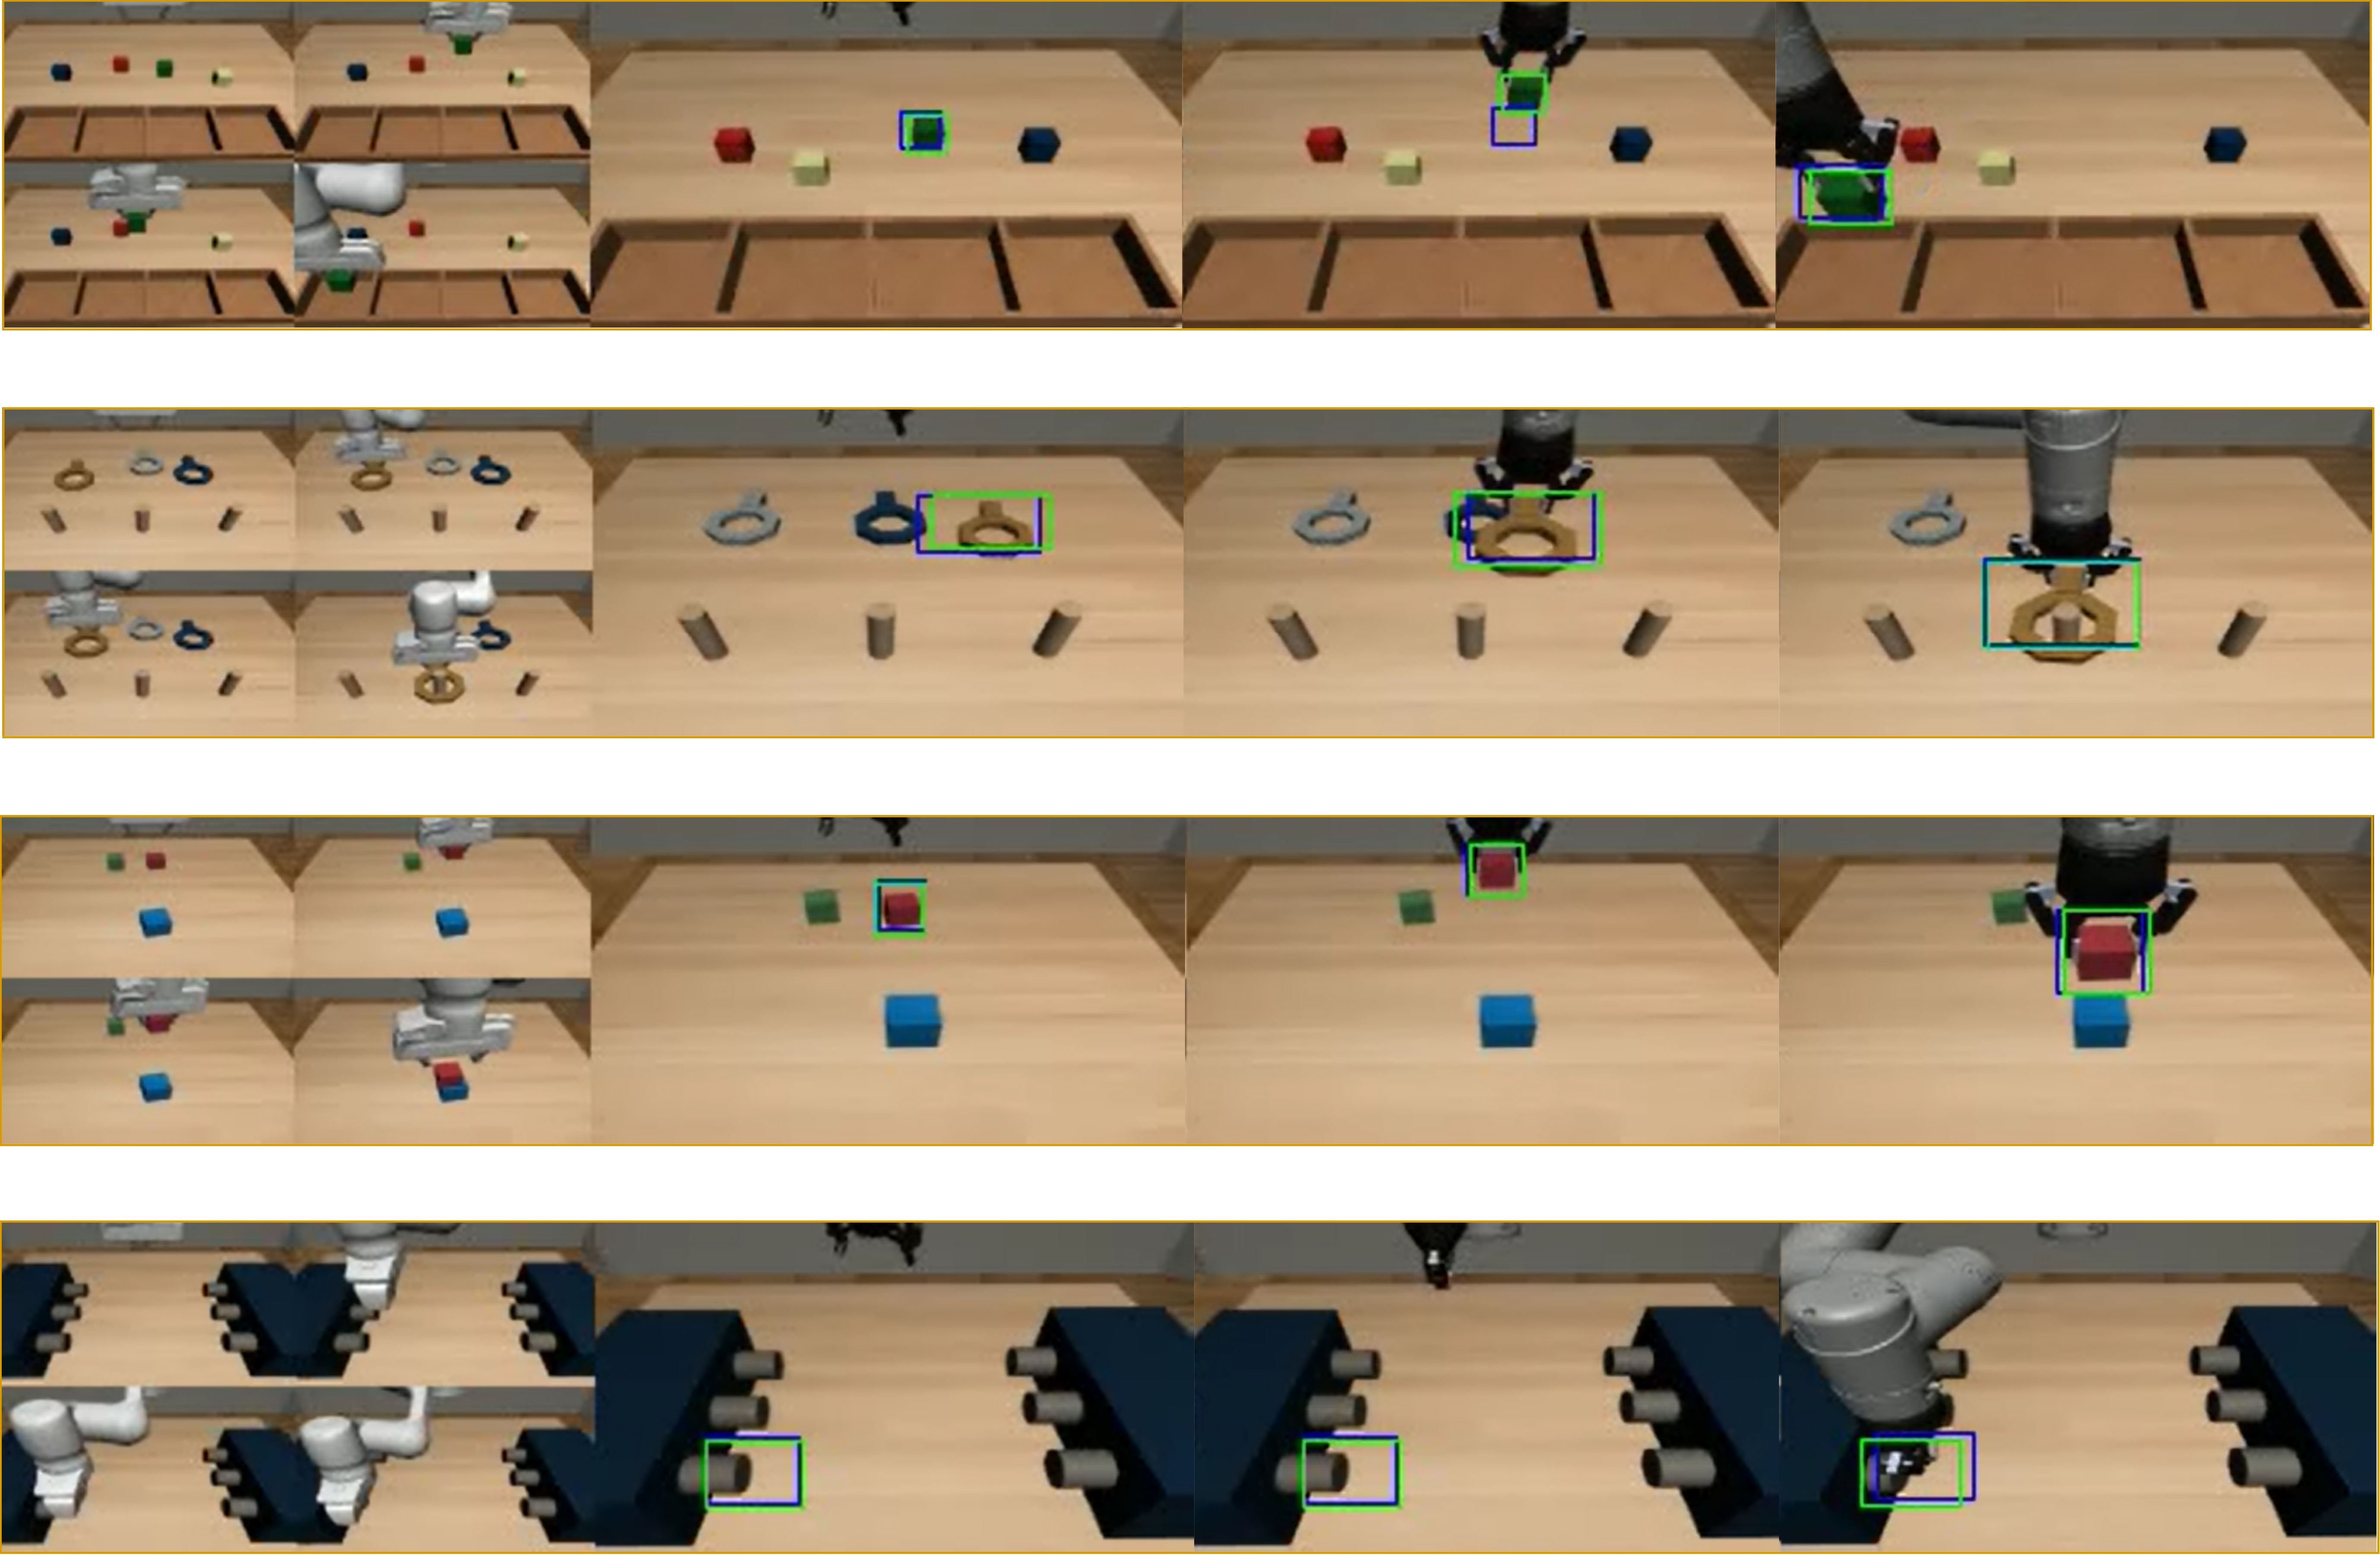
\includegraphics[width=1.0\textwidth]{figures/images/ch2/example_of_prediction_ctod_single.jpg}
    \caption{Example of predictions generated by the CTOD module in the single-task scenario. The blue-box is the predicted one, while the green is the ground truth.}
    \label{fig:ctod_example_of_prediction}
\end{figure}


\paragraph*{Multi-task multi-variation scenario}\mbox{}\\
In the multi-task multi-variation scenario, a single model was trained to perform all four tasks. This setup enables a more rigorous validation of the COD module in a complex environment, where objects of different shapes and sizes are involved across various tasks. Table \ref{table:ctod_multi_task_performance} presents the overall performance of the COD module in terms of Precision and Recall. In this scenario, the system consistently generates bounding boxes for the "target" class (achieving a Recall of 1.00 for all tasks) with an average overlap greater than 0.5. A similar trend as in the single-task scenario is observed, with a lower Precision for the Pick-Place task due to the same reasons previously explained.

Furthermore, compared to the single-task setting, a slight reduction in Average IoU is observed, which can be attributed to the increased complexity of the task. In this multi-task scenario, a single Fast R-CNN must predict bounding boxes across a diverse set of manipulation tasks, where objects may be similar but appear at different scales in the input images. This variation adds further complexity to the prediction process.


\subsubsection{Target object and final position detector}
\label{sec:cod_tofpd}
This set of validation tests focuses on training the COD module in the complete scenario described in Section \ref{sec:cod_problem}. In this setting, the COD module is trained to predict bounding boxes for both the target object and the final location of interest. Specifically, for the three tasks involving the ``pick-and-place" primitive (i.e., Pick-Place, Nut-Assembly, and Stack-Block), the final location corresponds to the target bin, peg, and block to be stacked, respectively. In contrast, for the Press-Button task, the target location is defined as the bounding box of the initial button, translated to the final position of the pressed button (Figure \ref{fig:press_button_target_placing}).
\begin{figure}[t]
    \centering
    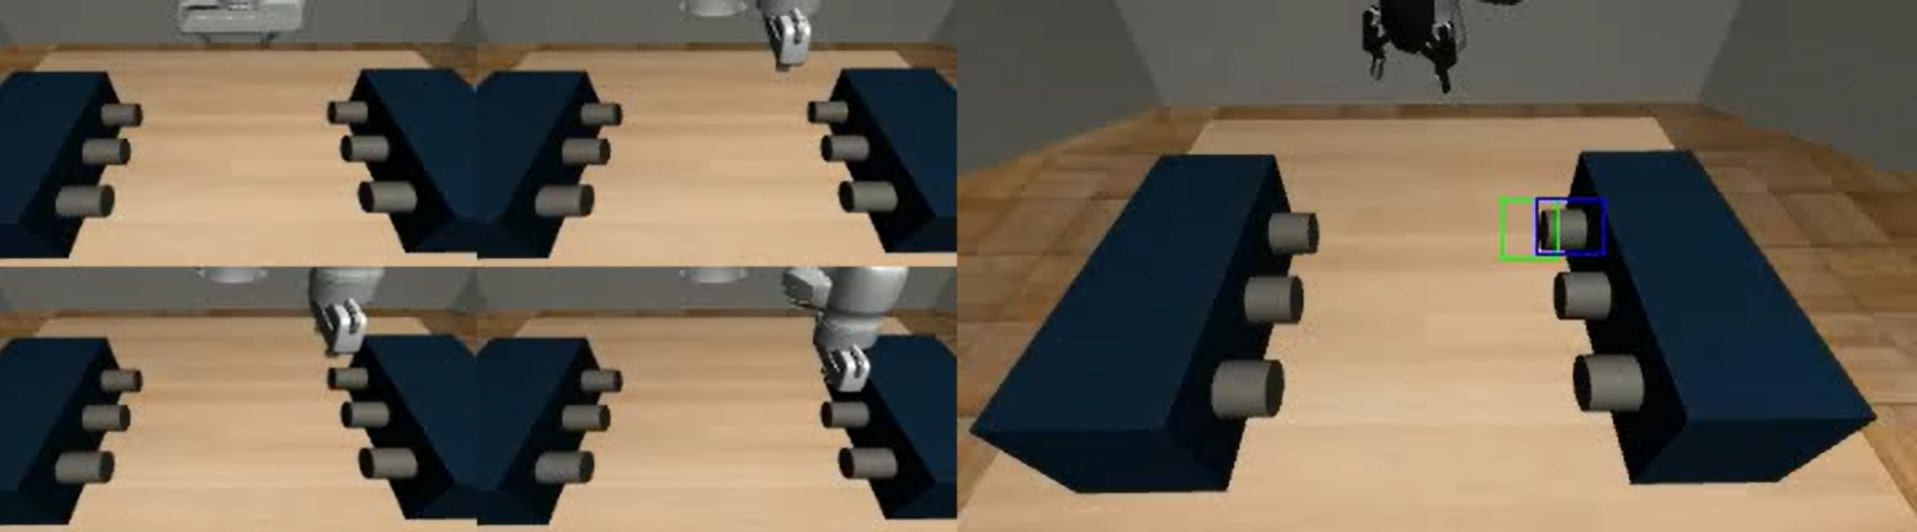
\includegraphics[width=0.9\textwidth]{figures/images/ch2/press_button_target_placing.jpg}
    \caption{Example of Target Bounding Box and Final Placing Position Definition for the Press-Button Task. In this task, the target bounding box is represented by the green bounding box, which encloses the button that needs to be pressed. The blue bounding box represents the final placing position, indicating the location where the robot's end-effector should be positioned to successfully press the button.}
    \label{fig:press_button_target_placing}
\end{figure}


\begin{table}[t]
    \centering
    \caption{Results of the COD module obtained in the single-task multi-variation scenario. Performances are reported in terms of \textit{Precision} (Prec), \textit{Recall} (Rec) with an IoU threshold of 0.5 and the Average IoU $(IoU_{avg})$ for both the bounding-box of the ``target" and the ``target-place" classes.}
    \label{table:cod_single_task_performance}
    \resizebox{\linewidth}{!}{%
    \begin{tabular}{|c|c|c|c|c|} 
    \hline
    \textbf{Task} & \textbf{Precision@0.5} & \textbf{Recall@0.5} & \begin{tabular}[c]{@{}c@{}}$\mathbf{IoU_{avg}}$~\\(target)\end{tabular} & \begin{tabular}[c]{@{}c@{}}$\mathbf{IoU_{avg}}$~\\(target-place)\end{tabular} \\ 
    \hhline{|=====|}
    Pick-Place & 0.667 & 1.00 & 0.374 & 0.826 \\ 
    \hline
    Nut-Assembly & 0.958 & 1.00 & 0.705 & 0.909 \\ 
    \hline
    Stack-Block & 0.979 & 1.00 & 0.787 & 0.827 \\ 
    \hline
    Press-Button & 0.967 & 1.00 & 0.799 & 0.683 \\
    \hline
    \end{tabular}
    }
    \end{table}
% \begin{table}[t]
%     \centering
%     \refstepcounter{table}
%     \caption{Distribution of the predicted bounding boxes generated by the CTOD module in the single-task, multi-variation scenario.}
%     \label{table:ctdo_single_task_prediction_distribution}
%     \resizebox{\linewidth}{!}{%
%     \begin{tabular}{|c|c|c|c|c|c|} 
%     \hline
%     \textbf{Task} & \textbf{TP} & \begin{tabular}[c]{@{}c@{}}\textbf{FP }\\\textbf{pre-picking}\end{tabular} & \begin{tabular}[c]{@{}c@{}}\textbf{FP }\\\textbf{post-picking}\end{tabular} & \begin{tabular}[c]{@{}c@{}}\textbf{FN }\\\textbf{pre-picking}\end{tabular} & \begin{tabular}[c]{@{}c@{}}\textbf{FN }\\\textbf{post-picking}\end{tabular} \\ 
%     \hhline{|======|}
%     \begin{tabular}[c]{@{}c@{}}Pick-Place \\(XXXX)\end{tabular} & XXXX & XXXX & XXXX & XXXX & XXXX \\ 
%     \hline
%     \begin{tabular}[c]{@{}c@{}}Nut-Assembly \\(XXXX)\end{tabular} & XXXX & XXXX & XXXX & XXXX & XXXX \\ 
%     \hline
%     \begin{tabular}[c]{@{}c@{}}Stack-Block\\(XXXX)\end{tabular} & XXXX & XXXX & XXXX & XXXX & XXXX \\ 
%     \hline
%     \begin{tabular}[c]{@{}c@{}}Press-Button\\(XXXX)\end{tabular} & XXXX & XXXX & XXXX & XXXX & XXXX \\
%     \hline
%     \end{tabular}
%     }
%     \end{table}

\begin{table}[t]
    \centering
    \caption{Results of the COD module obtained in the multi-task multi-variation scenario. Performances are reported in terms of \textit{Precision} (Prec), \textit{Recall} (Rec) with an IoU threshold of 0.5 and the Average IoU $(IoU_{avg})$ for both the bounding-box of the ``target'' and the ``target-place'' classes.}
    \label{table:cod_multi_task_performance}
    \resizebox{\linewidth}{!}{%
    \begin{tabular}{|c|c|c|c|c|} 
    \hline
    \textbf{Task} & \textbf{Precision@0.5} & \textbf{Recall@0.5} & \begin{tabular}[c]{@{}c@{}}$\mathbf{IoU_{avg}}$ \\~(target)\end{tabular} & \begin{tabular}[c]{@{}c@{}}$\mathbf{IoU_{avg}}$~\\(target-place)\end{tabular} \\ 
    \hhline{|=====|}
    Pick-Place & 0.735 & 1.00 & 0.457 & 0.825 \\ 
    \hline
    Nut-Assembly & 0.951 & 1.00 & 0.685 & 0.898 \\ 
    \hline
    Stack-Block & 0.867 & 1.00 & 0.628 & 0.799 \\ 
    \hline
    Press-Button & 0.925 & 1.00 & 0.734 & 0.687 \\
    \hline
    \end{tabular}
    }
    \end{table}
% \begin{table}[t]
%     \centering
%     \refstepcounter{table}
%     \caption{Distribution of the predicted bounding boxes generated by the CTOD module in the multi-task, multi-variation scenario.}
%     \label{table:ctdo_multi_task_prediction_distribution}
%     \resizebox{\linewidth}{!}{%
%     \begin{tabular}{|c|c|c|c|c|c|} 
%     \hline
%     \textbf{Task} & \textbf{TP} & \begin{tabular}[c]{@{}c@{}}\textbf{FP }\\\textbf{pre-picking}\end{tabular} & \begin{tabular}[c]{@{}c@{}}\textbf{FP }\\\textbf{post-picking}\end{tabular} & \begin{tabular}[c]{@{}c@{}}\textbf{FN }\\\textbf{pre-picking}\end{tabular} & \begin{tabular}[c]{@{}c@{}}\textbf{FN }\\\textbf{post-picking}\end{tabular} \\ 
%     \hhline{|======|}
%     \begin{tabular}[c]{@{}c@{}}Pick-Place \\(XXXX)\end{tabular} & XXXX & XXXX & XXXX & XXXX & XXXX \\ 
%     \hline
%     \begin{tabular}[c]{@{}c@{}}Nut-Assembly \\(XXXX)\end{tabular} & XXXX & XXXX & XXXX & XXXX & XXXX \\ 
%     \hline
%     \begin{tabular}[c]{@{}c@{}}Stack-Block\\(XXXX)\end{tabular} & XXXX & XXXX & XXXX & XXXX & XXXX \\ 
%     \hline
%     \begin{tabular}[c]{@{}c@{}}Press-Button\\(XXXX)\end{tabular} & XXXX & XXXX & XXXX & XXXX & XXXX \\
%     \hline
%     \end{tabular}
%     }
%     \end{table}
\paragraph*{Single-task multi-variation scenario}\mbox{}\\
Table \ref{table:cod_single_task_performance} summarizes the performance of the COD module in the single-task, multi-variation evaluation setting. It can be observed that, even in this scenario, the COD module consistently identifies both the target object and the target placement location. Specifically, the average Intersection over Union ($IoU_{avg}$) is generally higher for the target-placement class. This is because, for the Pick-Place, Nut-Assembly, and Stack-Block tasks, the placement location is fixed, making the detection problem easier for the conditioning module to address. 

Regarding the ``target" class, the $IoU_{avg}$ is lower compared to Table \ref{table:ctod_single_task_performance}, with a significant drop observed in the Pick-Place task. However, by examining the distribution of false positives, it can be noted that, out of \textbf{7565} false-positive cases, \textbf{2001} occurred during the reaching phase, while the remaining \textbf{5564} occurred during the placing phase. 

It is worth noting that the module can still identify the region of the target object. In fact, by lowering the IoU threshold to 0.1, the number of false positives during the reaching phase drops to 155, indicating that the system is able to detect the region of interest, albeit with lower precision. Nevertheless, for the task at hand, having consistently precise bounding boxes is not critical, as the control module is designed to be robust against minor errors or imprecisions in bounding box predictions.


\paragraph*{Multi-task multi-variation scenario}\mbox{}\\
The final evaluation setting essentially confirms the trends observed in the previous one. Table \ref{table:cod_multi_task_performance} summarizes the results obtained from the COD module trained in the multi-task scenario. In this case, a slight drop in Precision is again observed, which corresponds to a decrease in the average Intersection over Union ($IoU_{avg}$). This decline can be attributed to the same reasons discussed in the previous multi-task setting, with the added complexity that the module must also predict the bounding box for the target placement location.


In conclusion, this paragraph has introduced the COD module, a Conditioned-Convolutional Neural Network designed to address a novel object-detection problem. The module predicts category-agnostic bounding boxes for the two key regions in a manipulation task: the region where the object to be manipulated is located and the final region where the task is completed (e.g., placing the box, assembling the nut, stacking the block, or pressing the button). In a highly generalized multi-variation scenario, where the object position is not predefined and the semantic attribute assigned to the object is dynamically specified by a command, which is given through a video demonstration of another agent performing the desired task.


The results demonstrate that the proposed module effectively handles both single-task and multi-task scenarios, generating bounding boxes that are correctly classified and accurately identify the regions of interest.

In Chapter \ref{ch:occp}, it will be shown how the positional information from this command can be effectively utilized to inform the control module about the regions of interest, addressing the problem of target misidentification.


\section{Conclusion}
In conclusion, this chapter proposed and detailed the Conditioned Object Detector (COD), marking the first step in developing a modular architecture for Visual-Conditioned Multi-Task Imitation Learning. Specifically, this module addresses a key aspect of Cognitive Task design: identifying the region of interest in an agent's scene, based on a demonstrated task. The goal is to identify the relevant target object and final placement location in scenarios where multiple objects and placing locations are possible. The specific semantic attributes of these objects (i.e., target or distractor) are determined at runtime through task demonstration.

To tackle this challenge, a conditioned convolutional architecture was introduced and tested in both single-task multi-variation and multi-task multi-variation scenarios.

The results demonstrated that the proposed COD architecture effectively identified objects of interest, consistently achieving a Recall@0.5 score of \textbf{1.00} across all tasks and testing scenarios. This means that for every frame, a bounding box corresponding to the target class was always present.

Regarding Precision@0.5, there was variability across different tasks and scenarios, ranging from a minimum of \textbf{0.652} for the Pick-Place task in the multi-task multi-variation scenario to a maximum of \textbf{0.997} for the Press-Button task in the single-task multi-variation scenario. Despite this variation, the system was able to consistently identify the target object, with an average IoU always greater than 0.3. While this might appear low, further analysis of the generated bounding boxes revealed that the system successfully identified the target object during the initial stages of the rollout, particularly in the reaching phase, when conditioning on the target object is critical. However, a notable number of false positives occurred during the manipulation and placing phases, where the conditioning on the target object weakens, suggesting that the trained policy must be robust to errors in bounding box generation during these phases.
\chapter{Object conditioned control policy}
\label{ch:occp}
In this chapter the OCCP is going to be described. Specifically, Section~\ref{sec:ocpl_problem} will outline the problem being addressed. Section~\ref{sec:ocpl_architecture} will detail the proposed architecture designed to solve the described problem. Section~\ref{sec:ocpl_experimental} will discuss the experimental setup and present the results obtained from testing the proposed architecture.

\section{Problem formulation}
\label{sec:ocpl_problem}
As described in Section \ref{sec:occp_related_works}, this thesis primarily addresses the problem of Visual-Conditioned Multi-Task Imitation Learning. The goal is to train a single conditioned control function, $\pi_{\theta}(a_{t}| o^{a}_{t}, c_m)$, that can guide a robotic agent in solving both variations of a given task and entirely different tasks. Where, the input consists of a command $c_m$, represented as a video demonstration of the requested task, along with the current observation of the agent $o^{a}_{t}$.

The approach proposed in this thesis is based on the observation that solving this problem involves two key tasks:
\begin{itemize}
    \item \textit{Command analysis}: This task involves solving a cognitive problem, where the system must interpret the high-level task command, understand the task intent, identify the relevant objects, and recognize the required actions.
    \item \textit{Action generation}: This task involves solving a control problem, where the system must correlate the information from the command analysis with the agent environmental state to generate a valid action that moves the robot toward completing the requested task.
\end{itemize}

As demonstrated in the comprehensive review of related works (Section \ref{sec:occp_related_works}), the Visual-Conditioned MTIL problem is typically addressed using end-to-end architectures, which are trained with an action-centric behavioral cloning loss. While these systems are often able to control the robot and produce \textbf{reasonable trajectories} to complete tasks like pick-and-place, they may manipulate the wrong object, indicating a limitation in the cognitive ability to correctly identify the relevant object.


In this thesis, a modular approach is adopted. Specifically, Figure \ref{fig:end_to_end_vs_modular} illustrates the differences between a general end-to-end architecture and the proposed modular architecture. In the end-to-end architecture, the \textit{Backbone Module}, which can be any deep learning architecture used in state-of-the-art methods, takes both the agent observation $o^{a}_t$ and the command $c_{m_i}$ as input. It generates an embedding $z_t$ that must encapsulate all the necessary information for the \textit{Control Module} to produce a valid action. This includes details derived from both the command, such as the position of the object of interest, the task being solved, its variations, as well as the state of the agent itself.

In contrast, the modular approach utilizes two backbone modules. The first, the \textit{Command Analysis Backbone}, explicitly solves the cognitive task, producing task-relevant information ($z^{task}_t$) such as the position of the object of interest. The second, the \textit{Control Backbone Module}, generates a control embedding ($z^{control}_t$), which directly encodes information relevant to the action to be performed. In this modular approach, the \textit{Control Module} takes both the task-relevant information ($z^{task}_t$) and the control embedding ($z^{control}_t$) as inputs.

\begin{figure}[t]
    \centering
    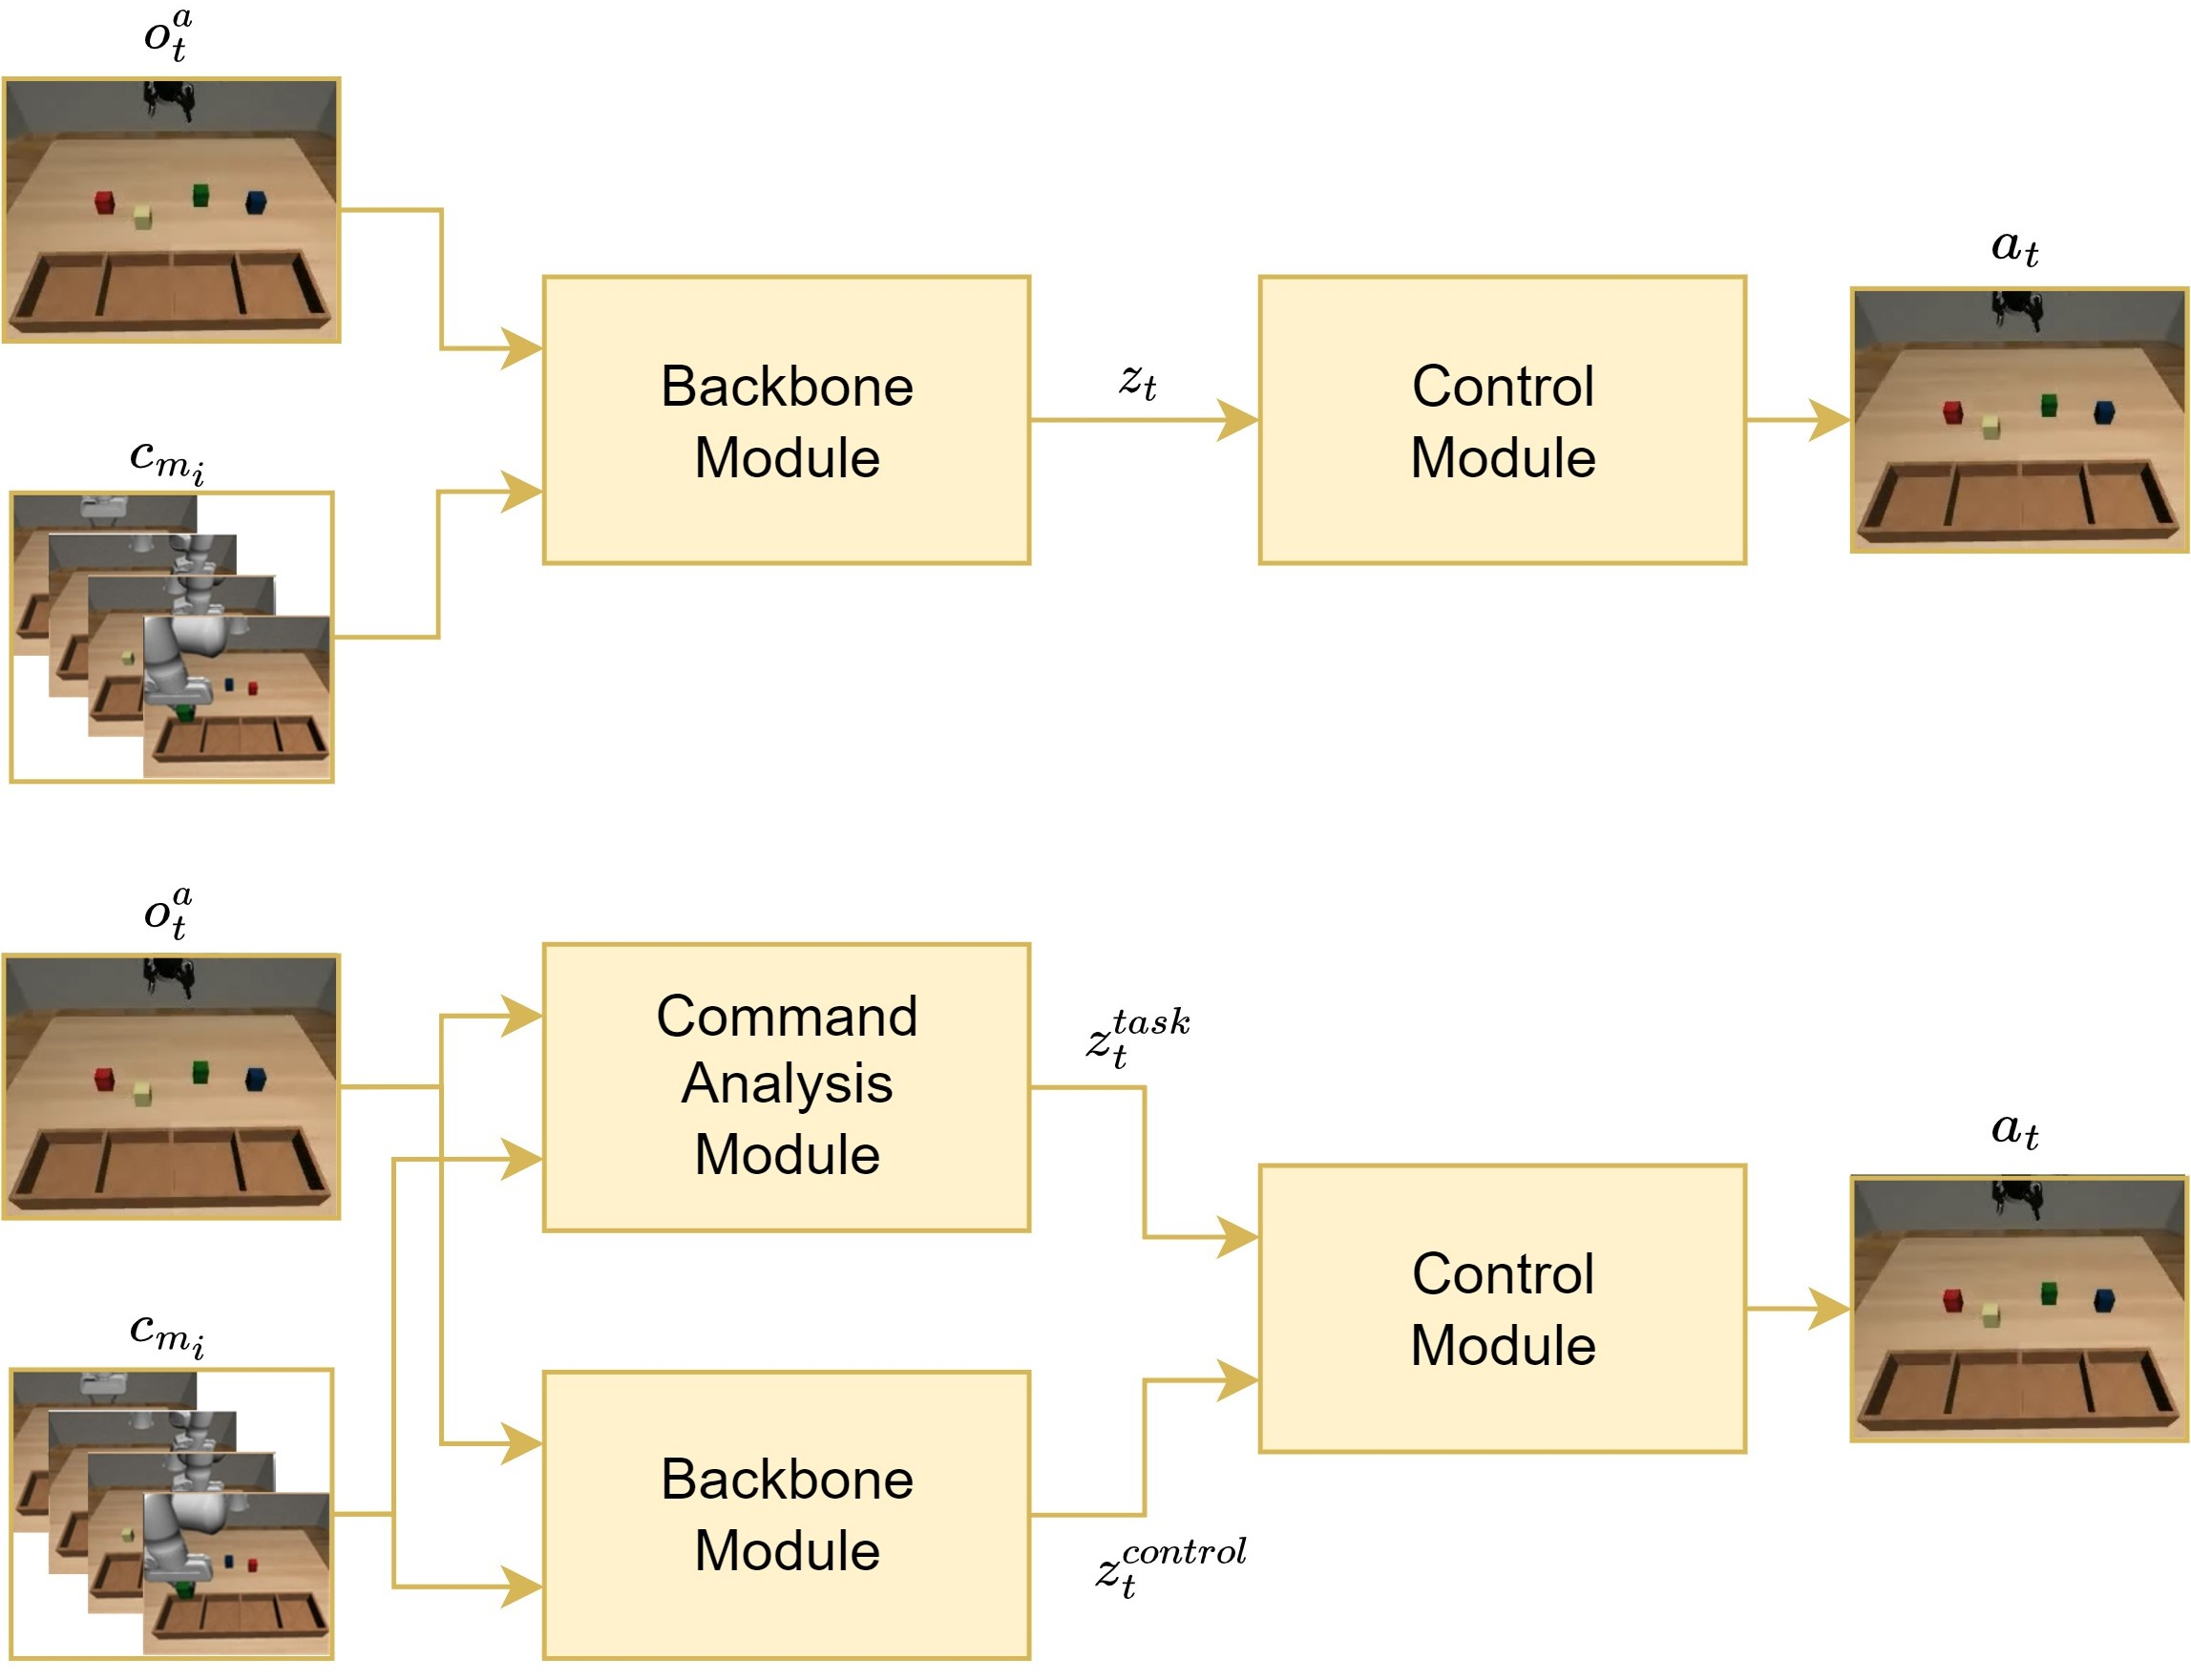
\includegraphics[width=0.7\textwidth]{figures/images/ch3/end_to_end_vs_modular.jpg}
    \caption{(Upper) General end-to-end architecture, where the \textit{Backbone Module} takes as input both the agent observation and the command. It generates an embedding $z_{t}$ that must contain information related to both the command and the control. (Bottom) In the modular architecture, there are two backbone modules: the \textit{Command Analysis Module}, which generates the task-embedding $z^{task}_t$, and the \textit{Backbone Module}, which is trained to generate only the control-embedding $z^{control}_{t}$.}
    \label{fig:end_to_end_vs_modular}
\end{figure}


The underlying assumption of this approach is that by separating the problem into two components, cognitive and control, and designing task-specific modules trained independently of each other, the system becomes more robust. For example, the Command Analysis Module is trained specifically for the cognitive task (e.g., the Conditioned Object Detection task described in Chapter \ref{ch:cod}), while the Control Backbone is trained for the control task. This separation allows the final Control Module to be informed by optimal embeddings generated by modules trained on task-specific problems.

Section \ref{sec:} provides an example of a cognitive problem that can be addressed by the Command Analysis Backbone. Here, the focus is on describing the problem solved in order to learn the final control policy $\pi_{\theta}$. Specifically, the goal is to learn the parameters of the policy $\pi_{\theta}$ using a supervised-learning approach.

The first step is defining the dataset. As explained in Section \ref{sec:bc}, in multi-task, multi-variation scenario, there are $n$ distinct tasks, denoted by $\mathcal{T} = \left\{T_{1}, T_{2}, \dots, T_{n}\right\}$, where each task $T_{i}$ is associated with a set of variations $\mathcal{M}_{i}$. For each task, a specific dataset $\mathcal{D}_{i} = ((c_{m}, \tau_{m}), m \in \mathcal{M}_{i})$ is constructed, containing pairs of demonstrator videos $c_{m}$ and corresponding target trajectories $\tau_{m}$ for each variation. The demonstrator video consists solely of visual observations, represented as $c_{m} = \left\{o^{d}_{1}, o^{d}_{2}, \dots, o^{d}_{T'}\right\}$, while the target trajectory includes both observations and associated actions: $\tau_{m} = \left\{(o^{a}_{1},a_{1}), \dots, (o^{a}_{T}, a_{T})\right\}$.

Building upon the complete dataset $\mathcal{D} = \left\{\mathcal{D}_{1}, \dots, \mathcal{D}_{n}\right\}$, the optimal parameters $\theta^{*}$ are obtained by solving the minimization problem described in Formula \ref{eq:minimization_prob}, where the loss function $\mathcal{L}$ is minimized.
\begin{equation}
    \label{eq:minimization_prob}
    \theta^{*} = \underset{\theta}{\text{arg} \ \min} \ \mathcal{L}(\pi_{\theta}, \mathcal{D})
\end{equation}

Section \ref{sec:ocpl_architecture} will present the specific instance of the proposed architecture, along with the loss function and modules used. The results of the experiments will be discussed in Section \ref{sec:ocpl_experimental}.

\section{Proposed Architecture}
\label{sec:ocpl_architecture}
This section provides the effective implementation of the general modular architecture described in Section \ref{sec:cod_problem}. Since the Command Analysis task being solved is Conditioned-Object Detection (Chapter \ref{ch:cod}), the focus here is on how the COD module is effectively integrated into the control framework.

The COD module is integrated into two different architectures, which vary in the number of control modules they use. Section~\ref{sec:ocpl_architecture_scm} outlines an architecture that employs a single control module to predict actions for the entire trajectory. In contrast, Section~\ref{sec:ocpl_architecture_dcm} describes an architecture that splits the control module into two distinct parts: one for computing actions during the reaching phase, and another for the final phase, where the specific primitive depends on the task.

\subsection{Single control module}
\label{sec:ocpl_architecture_scm}
The architecture (Figure \ref{fig:single_control_module}) composed of a single control module is essentially an instance of the general modular architecture depicted in Figure \ref{fig:end_to_end_vs_modular}. Specifically, the Command Analysis Module is replaced by the CTOD module (Section \ref{sec:cod_tod}), which takes as input the current agent observation $o^a_t$ and the command $c_m$, producing a task embedding represented by the \textit{target-object bounding box}, i.e., $z^{task}_t = bb^{target}_t$.

The Backbone Module, responsible for generating the control embedding $z^{control}_{t}$, is replaced by the same backbone used in MOSAIC. This backbone is a combination of a Convolutional Network, which encodes the agent observation $o^a_t$ and the demonstration frames $c_m$, and a Self-Attention mechanism to create correlated agent and command embeddings (Section \ref{sec:bc}). 

Finally, the Control Module follows the same implementation as in MOSAIC \cite{mandi2022towards_more_generalizable_one_shot}. In this case, the actions generated by the control module are sampled from a multivariate logistic distribution (Equation \ref{equation:logistic_distribution}), where the distribution parameters $\mu_{i}$ and $\sigma_{i}$ are estimated by MLPs implementing the Control Module.

\begin{equation}
    \label{equation:logistic_distribution}
    a_{t} \sim \sum_{i=1}^{m} \alpha(z_t) \, logistic(\mu_{i}(z_t), \sigma_{i}(z_t))
\end{equation}

Here, the embedding $z_t$ is a concatenation of $z^{control}_{t}$, generated by the MOSAIC Backbone, and $bb^{target}_t$, produced by the CTOD Module.

\begin{figure}[t]
    \centering
    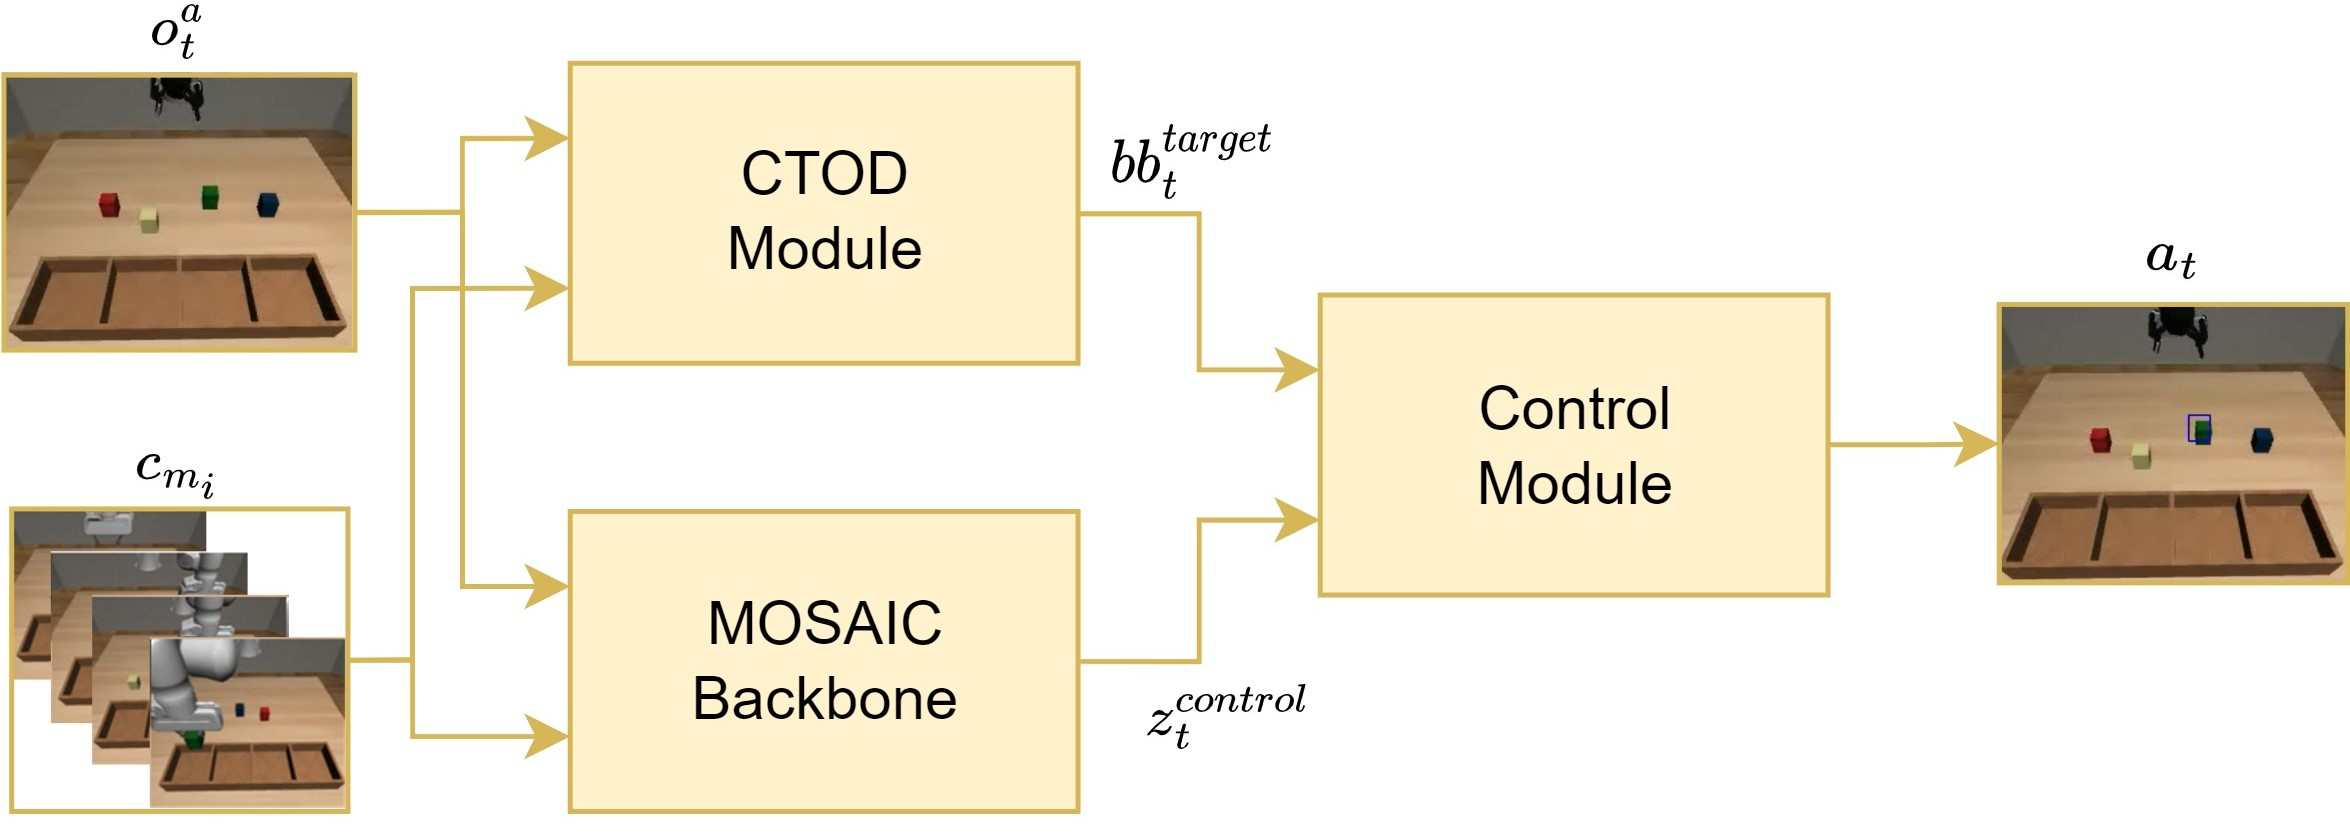
\includegraphics[width=0.9\textwidth]{figures/images/ch3/single_control_module.jpg}
    \caption{Proposed Single-Control Module Architecture. In contrast to the general architecture described in Figure \ref{fig:end_to_end_vs_modular}, the Command Analysis module is replaced by the CTOD module, which generates the bounding box related to the target object. The chosen backbone is the MOSAIC architecture \cite{mandi2022towards_more_generalizable_one_shot}. The control module is now informed by both low-level positional information ($bb^{target}_{t}$) and a control-oriented embedding ($z^{control}_{t}$), enabling it to make more informed decisions.}
    \label{fig:single_control_module}
\end{figure}


\subsection{Double control modules}
\label{sec:ocpl_architecture_dcm}
Regarding the architecture composed of multiple control modules, the discussion must begin with the key observation that the tasks considered can be roughly divided into two phases. The first is generally a \textit{reaching phase}, where the robot must reach a target location. The second phase varies based on the task: placing for Pick-Place, assembly for Nut-Assembly, stacking for Stack-Block, and pushing for Press-Button. Based on this, a dual control module architecture is proposed, with each control module trained to learn the primitive associated with each phase. The rationale behind this approach is that training modules specifically for simpler atomic primitives can result in a more robust and reliable control system.

Figure \ref{fig:double_control_module} illustrates the overall architecture. The main difference can be observed in the bounding boxes received by the control modules. Specifically, the MOSAIC Backbone generates the control embedding $z^{control}_t$, as before. However, the Command Analysis Module, now referred to as the COD Module, generates both the bounding box for the target object, $bb^{target}_t$, and the bounding box for the final placing position, $bb^{place}_t$. 

The $bb^{target}_t$ is provided as input to the \textit{Reaching Control} module, while the $bb^{place}_t$ is supplied to the \textit{Placing Control} module. 

Additionally, each control module operates based on an enabling signal $s^{en}$, which is set to 1 at the beginning of the rollout and remains active until the Reaching Control module generates its first prediction for the closing command. After this point, $s^{en}$ is set to 0, and control is transferred to the Placing Control module.    
\begin{figure}[t]
    \centering
    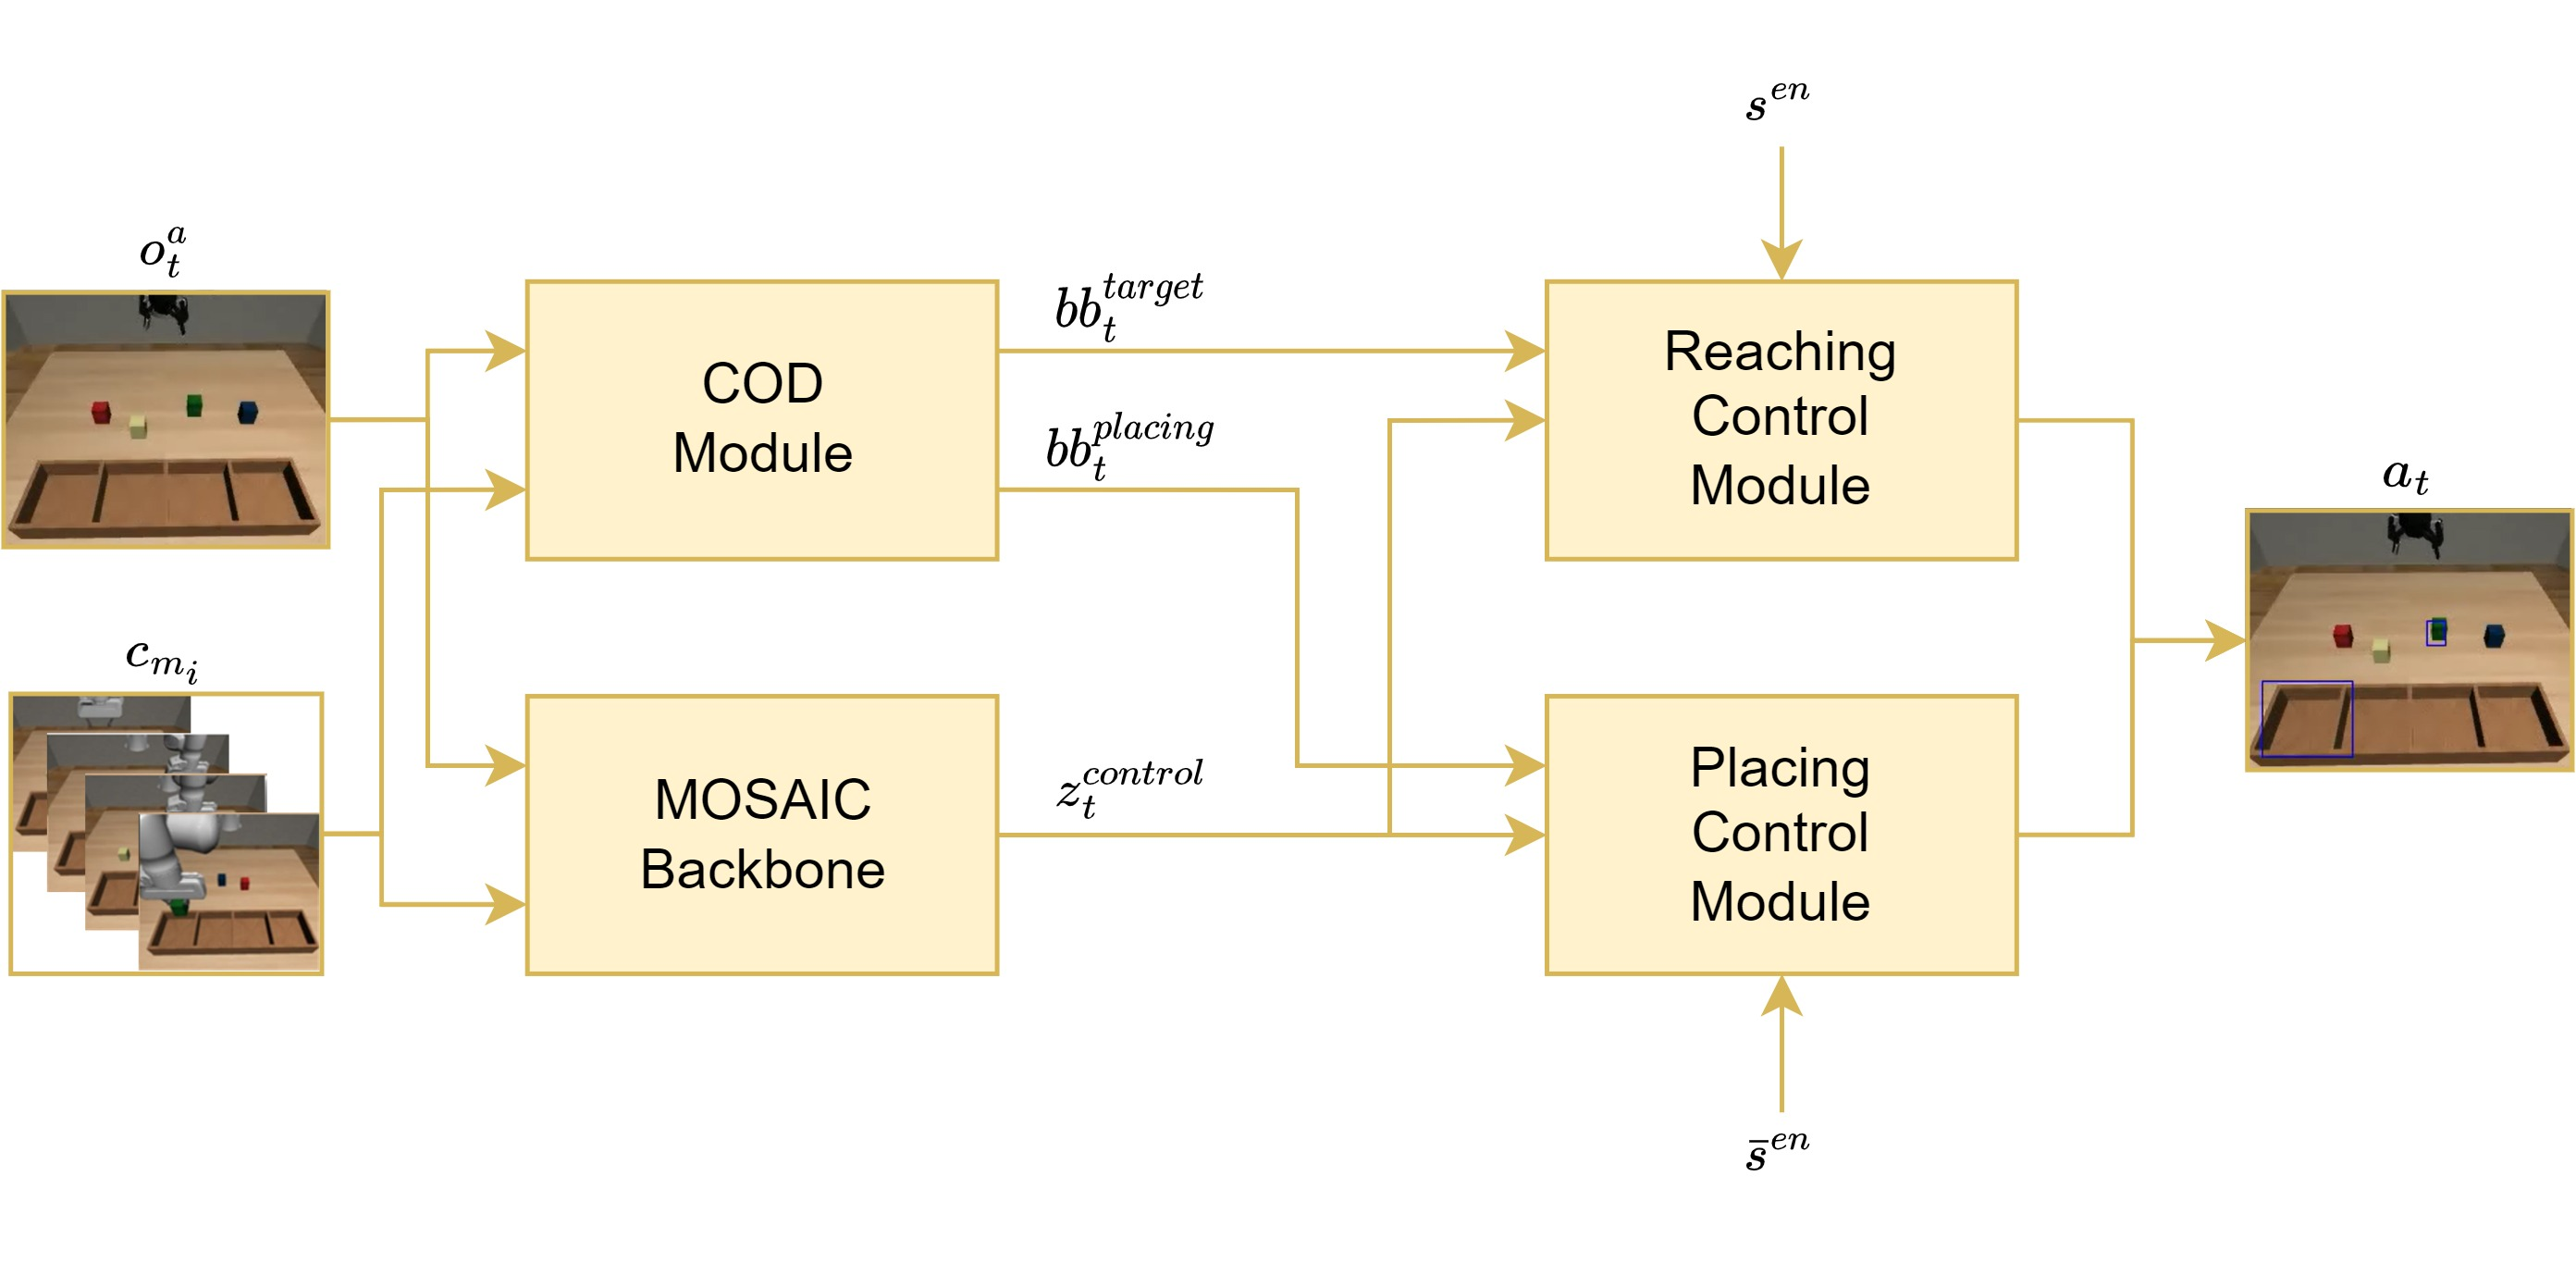
\includegraphics[width=0.9\textwidth]{figures/images/ch3/double_control_module.jpg}
    \caption{Proposed Double-Control Module Architecture. In this architecture, the Control Module is split into two distinct modules, each responsible for learning a specific primitive: the \textit{reaching} primitive and the \textit{placing} primitive. The first module takes as input the bounding box corresponding to the target object ($bb^{target}_{t}$), while the second module receives the bounding box related to the final placing location ($bb^{placing}_{t}$). This separation allows for specialized control during both the reaching and placing phases.}
    \label{fig:double_control_module}
\end{figure}

% \smalltodo{add figure}
\section{Experimental results}
\label{sec:ocpl_experimental}

In this section, the performed experiments are going to be described. Specifically, in  
Section~\ref{sec:ocpl_dataset} the dataset used for training procedure will be described. Section~\ref{sec:ocpl_results} will report the obtained results.
\begin{figure}[t]
    \centering
    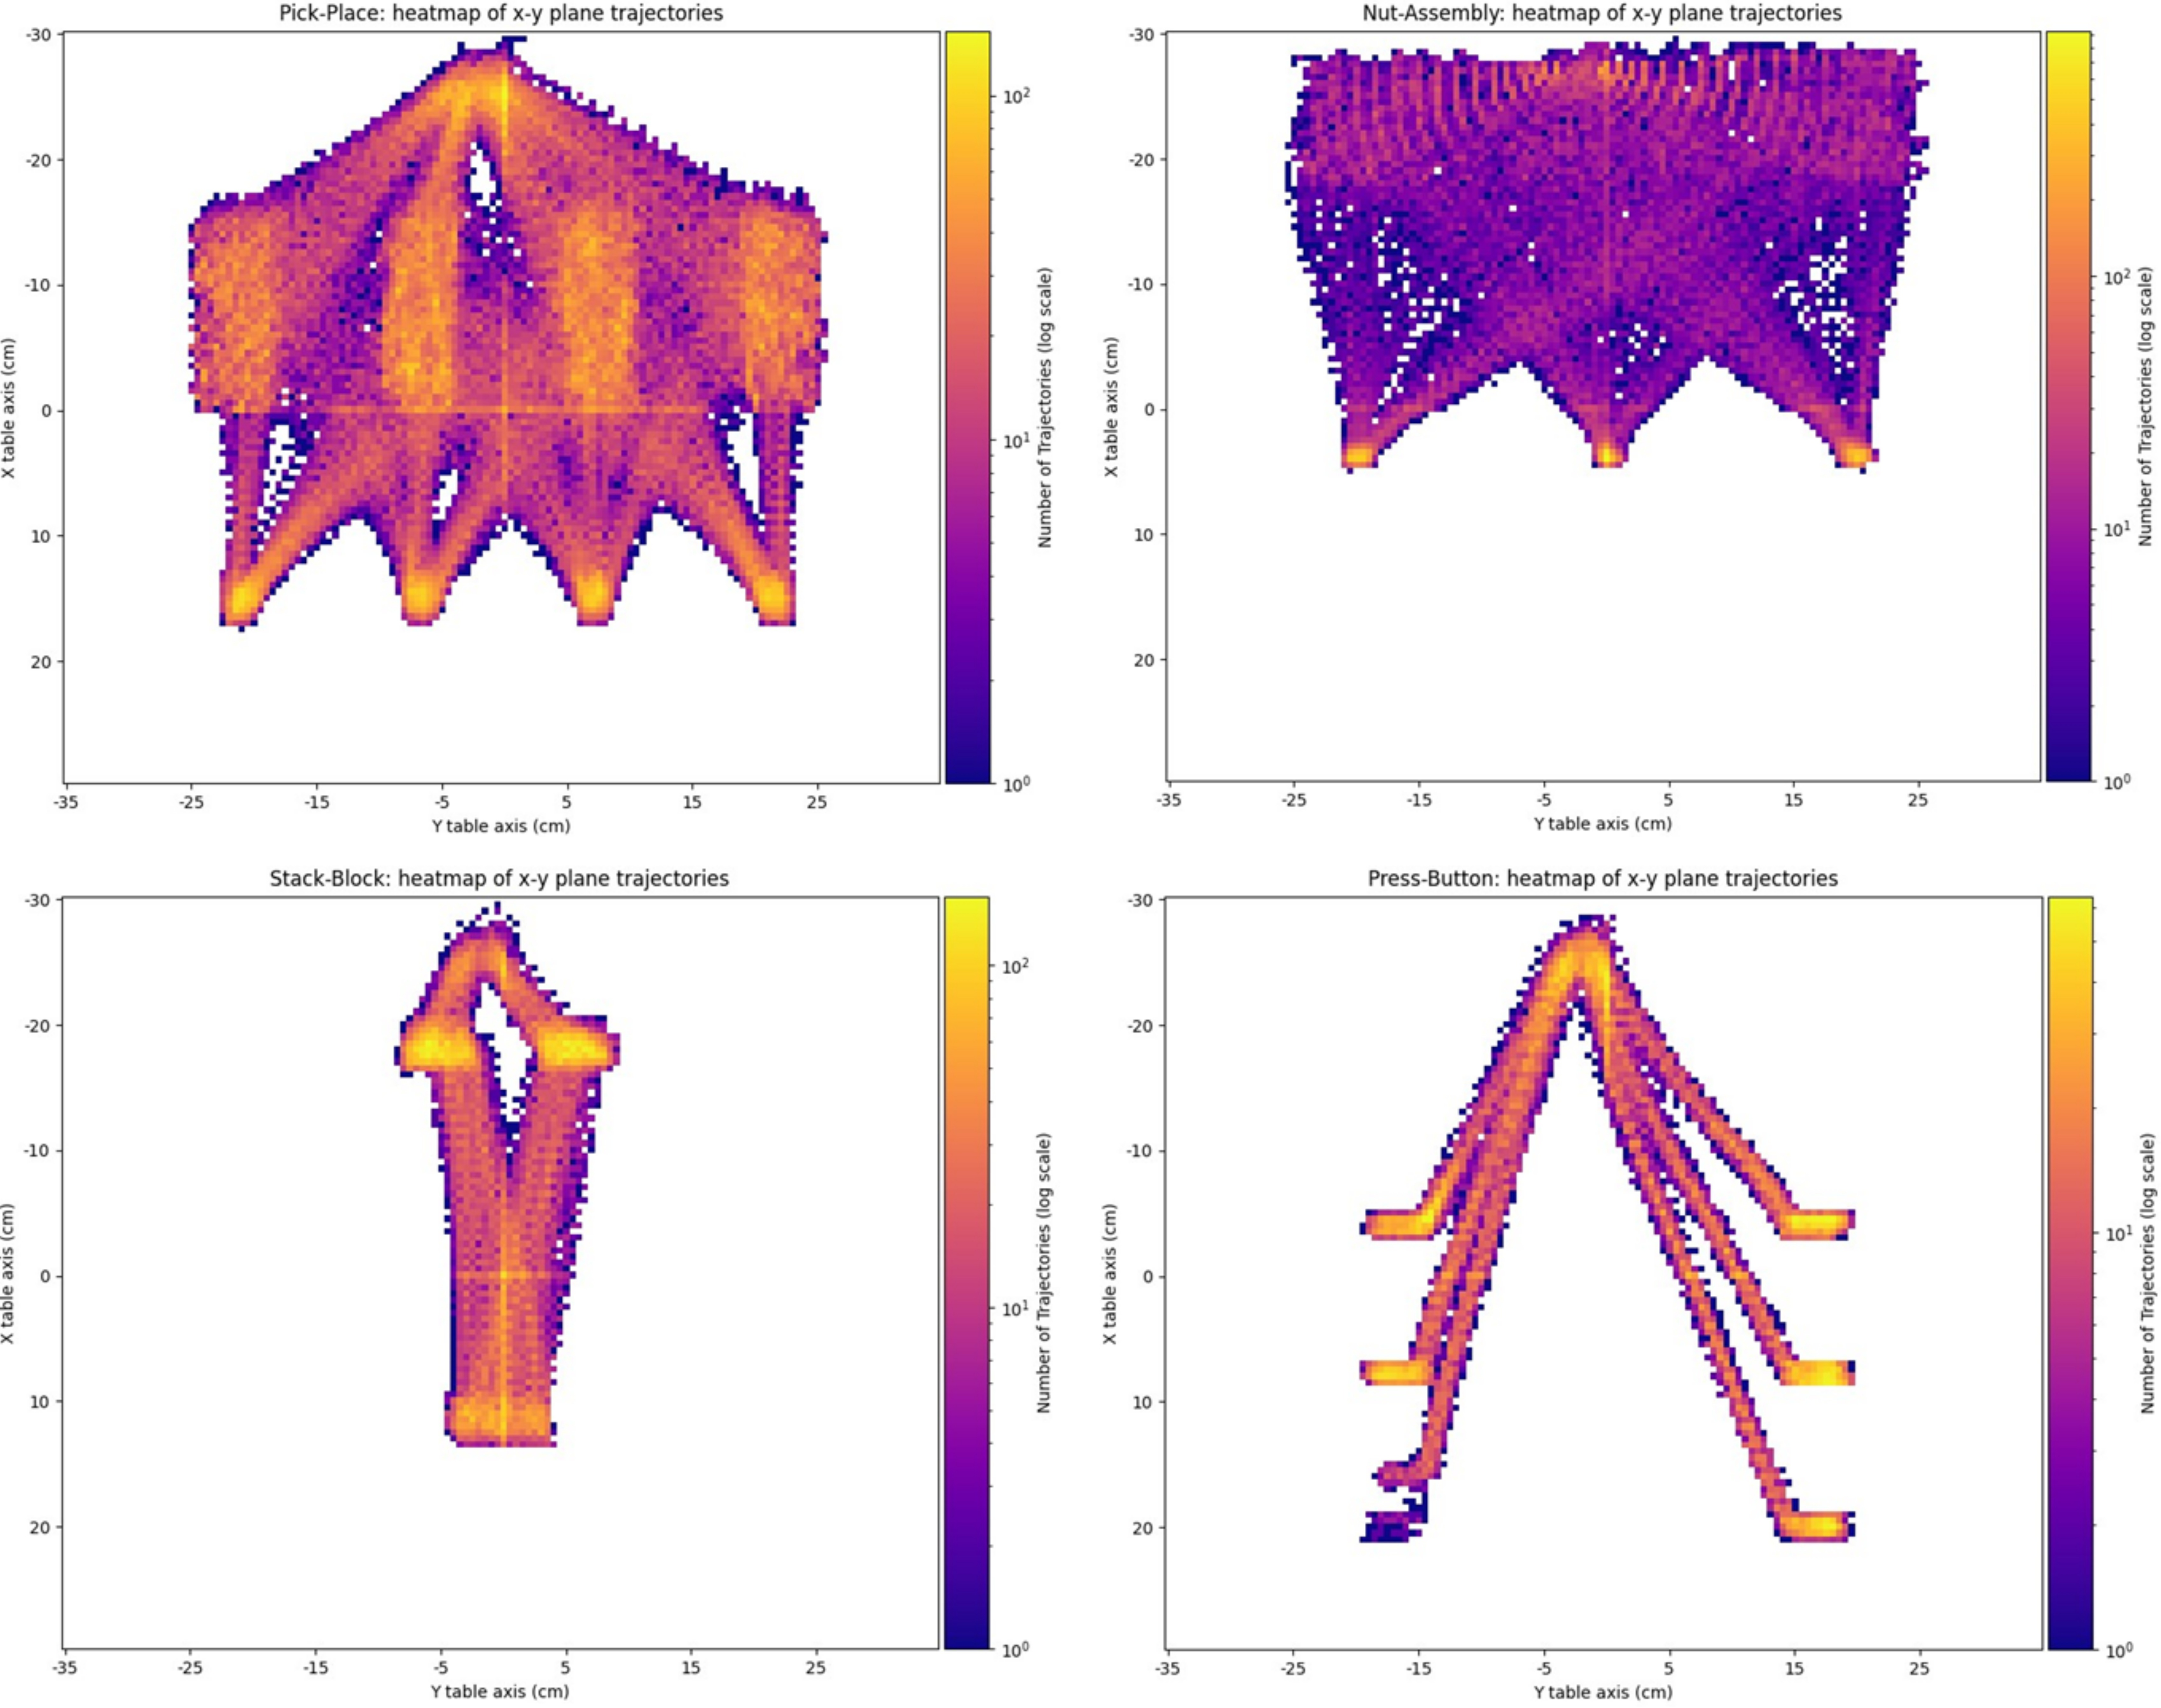
\includegraphics[width=1.0\textwidth]{figures/images/ch3/dataset_distribution.jpg}
    \caption{The distribution of trajectories for the different tasks along the x-y axis of the table workspace.}
    \label{fig:dataset_distribution}
\end{figure}

% The distribution of trajectories for the different tasks along the x-y axis of the table workspace. Each plot represents a density map illustrating the frequency with which the robot's end-effector passed through specific points across all variations and trajectories.
%  The tasks are organized as follows: (Top-Left) Pick-Place, (Top-Right) Nut-Assembly, (Bottom-Left) Stack-Block, and (Bottom-Right) Press-Button.

\subsection{Dataset}
\label{sec:ocpl_dataset}
The dataset used for training the control architectures is described in this section. It consists of the same tasks outlined in Section \ref{sec:cod_dataset}, following the same collection procedure. For each task variation, 100 trajectories were collected for both the agent and the demonstrator. Each trajectory presents a novel object configuration, according to the rules defined in Section \ref{sec:cod_dataset}.

In this section, the dataset is analyzed in terms of the distribution of the action space, in order to highlight the challenges from a control perspective.

Figure \ref{fig:dataset_distribution} illustrates the distribution of the trajectories followed by the robot. Each plot represents a density map illustrating the frequency with which the robot's end-effector passed through specific points across all variations and trajectories, specifically along the $x$ and $y$ axis. Notably, the use of a simulated environment enables complete coverage of the workspace. This particular aspect of the workspace coverage will be further discussed in Chapter \ref{ch:real_world_application} where the real-world system will be discussed.


% \smalltodo{Add figure here.}

Moreover, each task exhibits a \textbf{multi-modal behavior}. This is evident across different variations, as the final placing position changes with each variation. Additionally, during the reaching phase, the robot traverses almost all possible locations within the working area.

It is important to note that, for a given task, the trajectories exhibit significant variation in length. Specifically, for the Pick-Place task, the average trajectory length is \textbf{$71.21 \pm 7.69$} frames. In the Nut-Assembly task, the average length is \textbf{$62.24 \pm 7.47$} frames, while for the Stack-Block task, the average is \textbf{$63.07 \pm 1.51$} frames. Finally, in the Press-Button task, the average trajectory length is\textbf{ $40.45 \pm 8.17$} frames. 

This variability poses a challenge, as the likelihood of errors increases with task progression, and compounding errors become more pronounced over time. Additionally, this multi-modal behavior complicates the learning process. The dataset lacks any prior distribution (i.e., the robot does not consistently approach the target object from the same direction), making it challenging for the architecture to identify and leverage consistent patterns during training.

\subsection{Results}
\label{sec:ocpl_results}
This section presents the obtained results, divided into two main blocks. The first block (Section~\ref{sec:ocpl_results_scm}) discusses the results of the method described in Section\ref{sec:ocpl_architecture_scm}. The second block (Section~\ref{sec:ocpl_results_dcm}) covers the results of the method described in \ref{sec:ocpl_architecture_dcm}. For each method, results are reported for two different scenarios: first, where the method is trained in a single-task multi-variation scenario; and second, where the method is trained in a multi-task multi-variation scenario.

The tests are conducted following the procedure outlined in Section \ref{sec:cod_results}. For each variation, 10 independent runs are performed, each with a novel initial objects configuration. This approach assesses the system robustness with respect to different initial state configurations. Additionally, each set of 10 rollouts is repeated three times to evaluate the overall robustness and consistency of the model.

Various evaluation metrics are considered, either generally defined for each task or task-specific. The general metrics include:

\begin{itemize}
    \item \textit{Reaching}: The ratio of successful attempts where the robot reaches the target object across all rollouts.
    \item \textit{Picking}: The ratio of successful attempts where the robot picks the correct object across all rollouts.
    \item \textit{Success}: The ratio of successful task completions across all rollouts.
    \item \textit{Reaching Wrong}: The ratio of instances where the robot reaches an object other than the target across all rollouts.
    \item \textit{Picking Wrong}: The ratio of instances where the robot picks the wrong object across all rollouts.
    \item \textit{Success with Wrong Object}: The ratio of task completions where the robot manipulates the wrong object.
\end{itemize}

Task-specific metrics, particularly for tasks like Pick-Place and Nut-Assembly, include the 
\textit{Place Wrong with Correct Object} metric, which captures the number of times the robot places the correct object in the wrong position.
% \begin{itemize}
%     \item \textit{Place Wrong with Wrong Object}: The number of times the robot completes the task by placing the wrong object in the wrong position.
%     \item \textit{Place Wrong with Correct Object}: The number of times the robot completes the task by placing the correct object in the wrong position.
% \end{itemize}

These metrics provide a comprehensive evaluation of the robot performance, capturing all major error cases and giving a full picture of its behavior.

\subsubsection{Single control module}
In this section the results obtained with the architecture composed of a Single Control Module will be described. As in Chapter \ref{ch:cod}, there are two testing scenarios, the first one trained with a single-task  multi-variation scenario, while the second one with a multi-task multi-variation setting, with an increasing level of complexity.
\label{sec:ocpl_results_scm}
\paragraph*{Single-task multi-variation scenario}\mbox{}\\

The discussion of the results begins with the single-task multi-variation scenario, focusing on the baseline methods TOSIL \cite{dasari2021transformers_one_shot} and MOSAIC \cite{mandi2022towards_more_generalizable_one_shot}. Specifically, Table \ref{table:occp_single_task_baseline_res} presents the performance of these baseline methods. 
% \usepackage{makecell}
% \usepackage{graphicx}
% \usepackage{multirow}
% \usepackage{hhline}


\begin{table}[t]
    \centering
    % \refstepcounter{table}
    \label{table:occp_single_task_baseline_res}
    \caption{The single-task performance of the baseline methods, TOSIL \cite{dasari2021transformers_one_shot} and MOSAIC \cite{mandi2022towards_more_generalizable_one_shot}, was evaluated. For each model, additional tests were conducted by generating the first 2 steps and 10 steps using the hand-written controller.}
    \resizebox{\linewidth}{!}{%
    \begin{tabular}{|c|c|c|c|c|c|c|c|c|} 
    \hline
    \textbf{Task} & \textbf{Model} & \textbf{GT Action} & \begin{tabular}[c]{@{}c@{}}\textbf{Reaching}\\{[}\%]\end{tabular} & \begin{tabular}[c]{@{}c@{}}\textbf{Picking}\\{[}\%]\end{tabular} & \begin{tabular}[c]{@{}c@{}}\textbf{Success}\\{[}\%]\end{tabular} & \begin{tabular}[c]{@{}c@{}}\textbf{Reaching} \\\textbf{Wrong}~\\{[}\%]\end{tabular} & \begin{tabular}[c]{@{}c@{}}\textbf{Picking}\\\textbf{Wrong}\\{[}\%]\end{tabular} & \begin{tabular}[c]{@{}c@{}}\textbf{Success with}\\\textbf{Wrong Object}\\{[}\%]\end{tabular} \\ 
    \hhline{|=========|}
    \multirow{6}{*}{\rotatebox[origin=c]{90}{Pick-Place}} & \multirow{3}{*}{MOSAIC} & 0 & 62.90$\pm$0.95 & 62.08$\pm$0.95 & 58.75$\pm$1.87 & 36.67$\pm$0.95 & 36.67$\pm$0.95 & \textbf{37.71$\pm$0.72} \\ 
    \cline{3-9}
     & & 2 & 89.17$\pm$1.30 & 88.12$\pm$
      0.62 & 84.17$\pm$
      1.57 & 11.25$\pm$
      1.25 & 11.25$\pm$
      1.25 & 11.46$\pm$
      1.30 \\ 
    \cline{3-9}
     &  & 10 & 99.79$\pm$0.36 & 98.54$\pm$0.72 & \textbf{95.63$\pm$0.63} & 1.25$\pm$0.63 & 1.25$\pm$0.63 & 0.41$\pm$0.36 \\ 
    \cline{2-9}
     & \multirow{3}{*}{TOSIL} & 0 & 33.12$\pm$1.08 & 27.92$\pm$
      0.72 & 26.87$\pm$
      0.62 & 63.96$\pm$
      2.36 & 63.75$\pm$
      2.72 & \textbf{66.04$\pm$1.57} \\ 
    \cline{3-9}
     & & 2 & 69.17$\pm$1.30 & 60.83$\pm$2.52 & 59.38$\pm$2.17 & 29.17$\pm$0.95 & 28.96$\pm$1.30 & 30.83$\pm$2.20 \\ 
    \cline{3-9}
     &  & 10 & 98.58$\pm$0.36 & 92.71$\pm$
      1.44 & \textbf{90.00$\pm$1.08} & 2.70$\pm$
      1.30 & 2.70$\pm$
      1.30 & 1.25$\pm$
      0.62 \\ 
    \hhline{|=========|}
    \multirow{6}{*}{\rotatebox[origin=c]{90}{Nut-Assembly}} & \multirow{3}{*}{MOSAIC} & 0 & 38.89$\pm$1.11 & 36.67$\pm$1.11 & 33.33$\pm$1.11 & 59.26$\pm$1.69 & 55.93$\pm$1.69 & \textbf{51.48$\pm$2.31} \\ 
    \cline{3-9}
     & & 2 & 85.19$\pm$
      4.49 & 83.33$\pm$
      5.09 & 78.89$\pm$
      4.01 & 13.33$\pm$
      4.84 & 11.85$\pm$
      2.31 & 11.11$\pm$
      2.22 \\ 
    \cline{3-9}
     &  & 10 & 100.00$\pm$100.00 & 99.26$\pm$1.28 & \textbf{90.74$\pm$2.79} & 0.00$\pm$0.00 & 0.00$\pm$0.00 & 0.00$\pm$0.00 \\ 
    \cline{2-9}
     & \multirow{3}{*}{TOSIL} & 0 & 36.30$\pm$
      1.28 & 35.19$\pm$
      2.31 & 31.11$\pm$
      1.92 & 63.33$\pm$
      1.11 & 62.59$\pm$
      1.28 & \textbf{56.30$\pm$3.57} \\ 
    \cline{3-9}
     & & 2 & 83.33$\pm$2.22 & 82.96$\pm$2.31 & 77.78$\pm$2.22 & 16.67$\pm$2.22 & 16.67$\pm$2.22 & 14.44$\pm$1.11 \\ 
    \cline{3-9}
     &  & 10 & 100.00$\pm$
      0.00 & 99.26$\pm$
      1.28 & \textbf{88.89$\pm$2.22} & 0.00$\pm$
      0.00 & 0.00$\pm$
      0.00 & 0.00$\pm$
      0.00 \\ 
    \hhline{|=========|}
    \multirow{6}{*}{\rotatebox[origin=c]{90}{Stack-Block}} & \multirow{3}{*}{MOSAIC} & 0 & 60.56$\pm$0.96 & 60.56$\pm$0.96 & 53.33$\pm$1.66 & 39.44$\pm$0.96 & 39.44$\pm$0.96 & \textbf{36.11$\pm$0.96} \\ 
    \cline{3-9}
     & & 2 & 91.11$\pm$
      0.96 & 90.56$\pm$
      0.96 & 73.89$\pm$
      4.19 & 7.70$\pm$
      0.96 & 7.70$\pm$
      0.96 & 7.20$\pm$
      0.96 \\ 
    \cline{3-9}
     &  & 10 & 100.00$\pm$0.00 & 99.44$\pm$0.96 & \textbf{77.78$\pm$1.92} & 0.00$\pm$0.00 & 0.00$\pm$0.00 & 0.00$\pm$0.00 \\ 
    \cline{2-9}
     & \multirow{3}{*}{TOSIL} & 0 & 69.44$\pm$
      0.96 & 60.00$\pm$
      0.16 & 48.89$\pm$
      2.54 & 42.78$\pm$
      0.96 & 42.78$\pm$
      0.96 & \textbf{41.67$\pm$1.66} \\ 
    \cline{3-9}
     & & 2 & 90.56$\pm$0.96 & 87.78$\pm$0.96 & 79.44$\pm$1.92 & 12.22$\pm$0.96 & 11.67$\pm$0.00 & 11.67$\pm$0.00 \\ 
    \cline{3-9}
     &  & 10 & 100.00$\pm$
      0.00 & 99.44$\pm$
      0.96 & \textbf{88.89$\pm$1.92} & 1.66$\pm$
      1.66 & 1.11$\pm$
      0.96 & 0.00$\pm$
      0.00 \\ 
    \hhline{|=========|}
    \multirow{6}{*}{\rotatebox[origin=c]{90}{Press-Button}} & \multirow{3}{*}{MOSAIC} & 0 & 100.00$\pm$0.00 & - & \textbf{100.00$\pm$0.00} & 0.00$\pm$0.00 & - & 0.00$\pm$0.00 \\ 
    \cline{3-9}
     & & 2 & 100.00$\pm$
      0.00 & - & 100.00,
      0.00 & 0.00$\pm$
      0.00 & - & 0.00$\pm$
      0.00 \\ 
    \cline{3-9}
     &  & 10 & 100.00$\pm$0.00 & - & 100.00$\pm$0.00 & 0.00$\pm$0.00 & - & 0.00$\pm$0.00 \\ 
    \cline{2-9}
     & \multirow{3}{*}{TOSIL} & 0 & 83.33$\pm$
      1.66 & - & \textbf{83.33$\pm$1.66} & 17.78$\pm$
      1.93 & - & 16.67$\pm$
      1.67 \\ 
    \cline{3-9}
     & & 2 & 80.56$\pm$1.92 & - & 80.56$\pm$1.92 & 20.00$\pm$2.88 & - & 18.33$\pm$2.89 \\ 
    \cline{3-9}
     &  & 10 & 92.22$\pm$
      0.96 & - & 81.67$\pm$
      3.33 & 9.44$\pm$
      0.96 & - & 9.44$\pm$
      0.96 \\
    \hline
    \end{tabular}
    }
    \end{table}

As observed, both baseline methods suffer from the issue of \textbf{target-object misidentification}. This is evident from the \textit{Success with Wrong Object} column, where the success rate involving wrong objects is significant. Figure \ref{fig:baseline_pick_place_error} provides an example of a pick-and-place rollout in which the task is technically completed, but the wrong object is manipulated.
\begin{figure}[t]
    \centering
    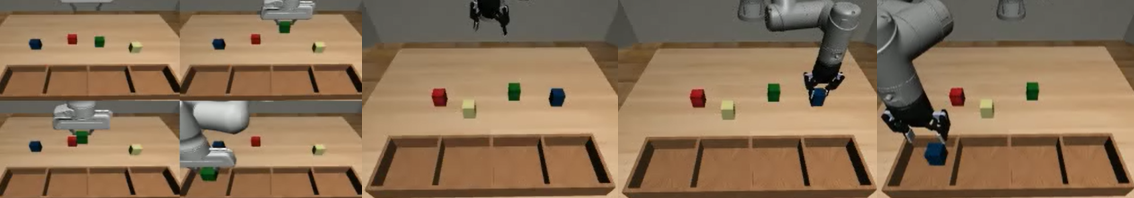
\includegraphics[width=1.0\textwidth]{figures/images/baseline_pick_place_error/pick_place_trj.png}
    \caption{Example of task rollout with incorrect object manipulation. In this scenario, the robot successfully completes the task by placing an object in the first bin. However, instead of manipulating the correct object (the green box), the robot mistakenly picks up the blue box. This illustrates a situation where the robot executes the task's final action correctly but selects the wrong object during manipulation.}
    \label{fig:baseline_pick_place_error}
\end{figure}

% \smalltodo{Add Figure}

To investigate the cause of these errors, test rollouts were conducted using the first 2 and 10 actions generated by a hand-written policy with access to ground-state information. Notably, the success rate improves significantly by applying just 2 ground-truth actions. This observation supports the hypothesis outlined in Section \ref{sec:ocpl_problem}, suggesting that the end-to-end architecture trained with an action-centric loss produces a suboptimal embedding $z$ for the cognitive task. Specifically, the embedding does not adequately inform the control policy about the correct position of the target object.

Based on this consideration, the thesis proposal to inform the control module with both a low-level positional information (e.g., the bouding-box of the target object) and a control embedding generated by the MOSAIC-backbone has been tested. During this test, two models variations have been considered, the first named \textit{MOSAIC-GT-BB} is basically the MOSAIC model, with the Control Module that receives in input the control-embedding $z^{control}$ and the ground-truth bouding-box. The second, named \textit{MOSAIC-CTOD} is the architecture described in Section \ref{sec:ocpl_architecture_scm}.

\begin{table}[t]
  \centering
  \caption{The single-task performance of the proposed MOSAIC-CTOD module is compared to the MOSAIC and MOSAIC-GT-BB baselines. MOSAIC-GT-BB refers to the MOSAIC model, where the Control Module receives the ground-truth target bounding box as input.}
  \label{table:ctod_single_task}
  \resizebox{\linewidth}{!}{%
  \begin{tabular}{|c|c|c|c|c|c|c|c|} 
  \hline
  \textbf{Task} & \textbf{Method} & \begin{tabular}[c]{@{}c@{}}\textbf{Reaching}\\{[}\%]\end{tabular} & \begin{tabular}[c]{@{}c@{}}\textbf{Picking}\\{[}\%]\end{tabular} & \begin{tabular}[c]{@{}c@{}}\textbf{Success}\\{[}\%]\end{tabular} & \begin{tabular}[c]{@{}c@{}}\textbf{Reaching }\\\textbf{Wrong~}\\{[}\%]\end{tabular} & \begin{tabular}[c]{@{}c@{}}\textbf{Picking}\\\textbf{Wrong}\\{[}\%]\end{tabular} & \begin{tabular}[c]{@{}c@{}}\textbf{Success with}\\\textbf{Wrong Object}\\{[}\%]\end{tabular} \\ 
  \hhline{|========|}
  \multirow{3}{*}{Pick-Place} & MOSAIC & 62.90$\pm$0.95 & 62.08$\pm$0.95 & 58.75$\pm$1.87 & 36.67$\pm$0.95 & 36.67$\pm$0.95 & 37.71$\pm$0.72 \\ 
  \cline{2-8}
   & MOSAIC-GT-BB & 100.00$\pm$   0.00 & 97.71$\pm$   0.72 & 76.46$\pm$   3.20 & 0.00$\pm$   0.00 & 0.00$\pm$   0.00 & 0.00$\pm$   0.00 \\ 
  \cline{2-8}
   & MOSAIC-CTOD & 98.12$\pm$0.62 & 91.88$\pm$4.88 & \textbf{77.11$\pm$5.60} & 1.04$\pm$0.36 & 1.04$\pm$0.36 & 1.04$\pm$0.36 \\ 
  \hhline{|========|}
  \multirow{3}{*}{Nut-Assembly} & MOSAIC & 38.89$\pm$1.11 & 36.67$\pm$1.11 & 33.33$\pm$1.11 & 59.26$\pm$1.69 & 55.93$\pm$1.69 & 51.48$\pm$2.31 \\ 
  \cline{2-8}
   & MOSAIC-GT-BB & 100.00$\pm$   0.00 & 98.89$\pm$   1.11 & \textbf{70.37$\pm$1.69} & 0.00$\pm$   0.00 & 0.00$\pm$   0.00 & 0.00$\pm$   0.00 \\ 
  \cline{2-8}
   & MOSAIC-CTOD & 98.89$\pm$1.11 & 97.41$\pm$2.31 & 64.07$\pm$0.64 & 0.00$\pm$0.00 & 0.00$\pm$0.00 & 0.00$\pm$0.00 \\ 
  \hhline{|========|}
  \multirow{3}{*}{Stack-Block} & MOSAIC & 60.56$\pm$0.96 & 60.56$\pm$0.96 & 53.33$\pm$1.66 & 39.44$\pm$0.96 & 39.44$\pm$0.96 & 36.11$\pm$0.96 \\ 
  \cline{2-8}
   & MOSAIC-GT-BB & 100.00$\pm$   0.00 & 99.44$\pm$   0.96 & 90.00$\pm$   2.89 & 0.00$\pm$   0.00 & 0.00$\pm$   0.00 & 0.00$\pm$   0.00 \\ 
  \cline{2-8}
   & MOSAIC-CTOD & 100.00$\pm$0.00 & 100.00$\pm$0.00 & \textbf{91.67$\pm$2.88} & 0.00$\pm$0.00 & 0.00$\pm$0.00 & 0.00$\pm$0.00 \\ 
  \hhline{|========|}
  \multirow{3}{*}{Press-Button} & MOSAIC & 100.00$\pm$0.00 & - & \textbf{100.00$\pm$0.00} & 0.00$\pm$0.00 & - & 0.00$\pm$0.00 \\ 
  \cline{2-8}
   & MOSAIC-GT-BB & 92.22$\pm$   2.54 & - & 90.56$\pm$   1.92 & 3.88$\pm$   0.96 & - & 3.88$\pm$   0.96 \\ 
  \cline{2-8}
   & MOSAIC-CTOD & 97.22$\pm$1.92 & - & 95.56$\pm$1.92 & 2.77$\pm$0.96 & - & 2.77$\pm$0.96 \\
  \hline
  \end{tabular}
  }
  \end{table}
The results are summarized in Table \ref{table:ctod_single_task_performance}. Several key observations can be made from these findings. For tasks involving multiple similar objects that change positions across different demonstrations (such as Pick-Place, Nut-Assembly, and Stack-Block), the use of positional information significantly enhances the system robustness. This enables the robot to consistently reach the target object and improves the overall success rate.

In contrast, for the Press-Button task, while the MOSAIC-CTOD method achieves a high success rate (95.56\% on average), it does not overcome the baseline method, which consistently solves the task with a 100\% success rate. This limitation arises because, once the button is reached, the positional information provides no further guidance on how to complete the task. Consequently, the robot often gets stuck near the button, failing to execute the pushing action (Figure \ref{fig:button_ctod_error}).
\begin{figure}[t]
    \centering
    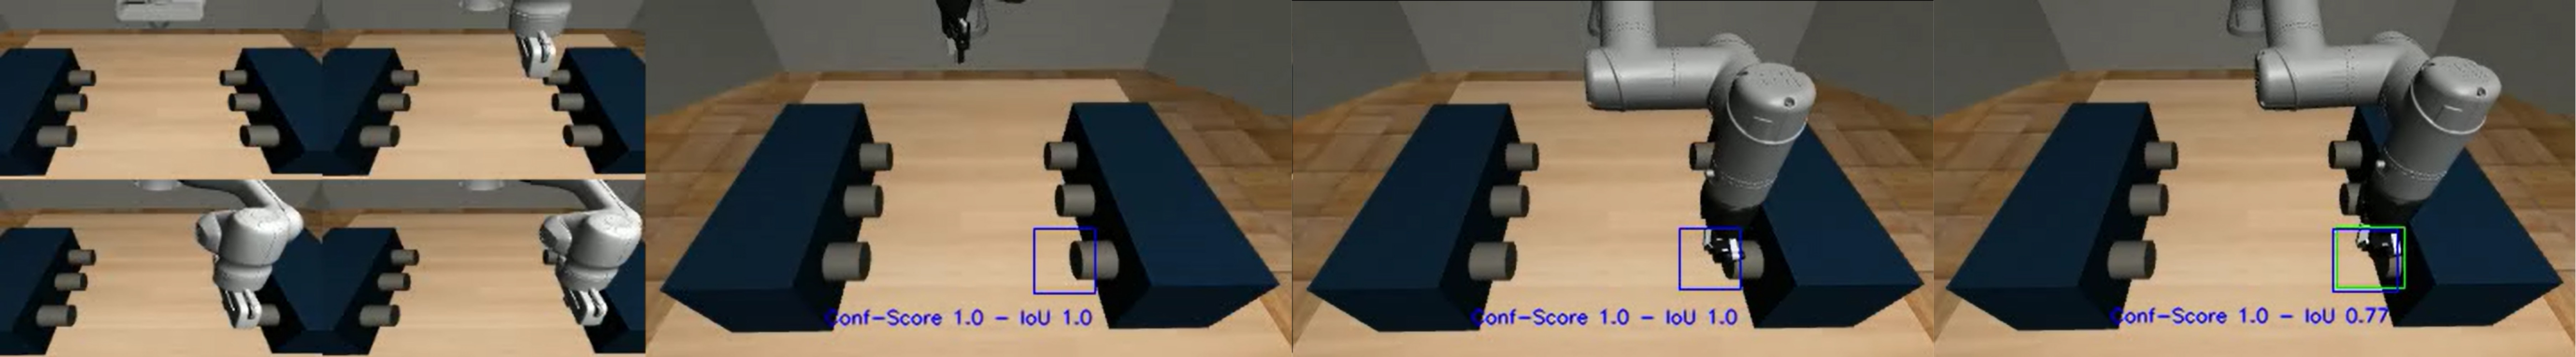
\includegraphics[width=1.0\textwidth]{figures/images/ch3/button_error.jpg}
    \caption{Example of unsuccessful Press-Button rollout. In this scenario, the robot successfully reaches the target button using the predicted bounding box (blue). However, due to instability in predictions during the pushing phase, the robot is unable to complete the pressing action, resulting in an unsuccessful task execution.}
    \label{fig:button_ctod_error}
\end{figure}

% \smalltodo{Add Figure}

Furthermore, the inclusion of positional information introduces a novel type of error. Specifically, since the robot behavior is conditioned by the bounding box, any error in its prediction can cause the robot to move incorrectly (Figure \ref{fig:error_propagation}). This error is significant, as in the Pick-Place task, the metric ``Place Wrong with Correct Object" reaches 11.25\%, and for the Nut-Assembly task, the same metric averages 22.22\%.
\begin{figure}[t]
    \centering
    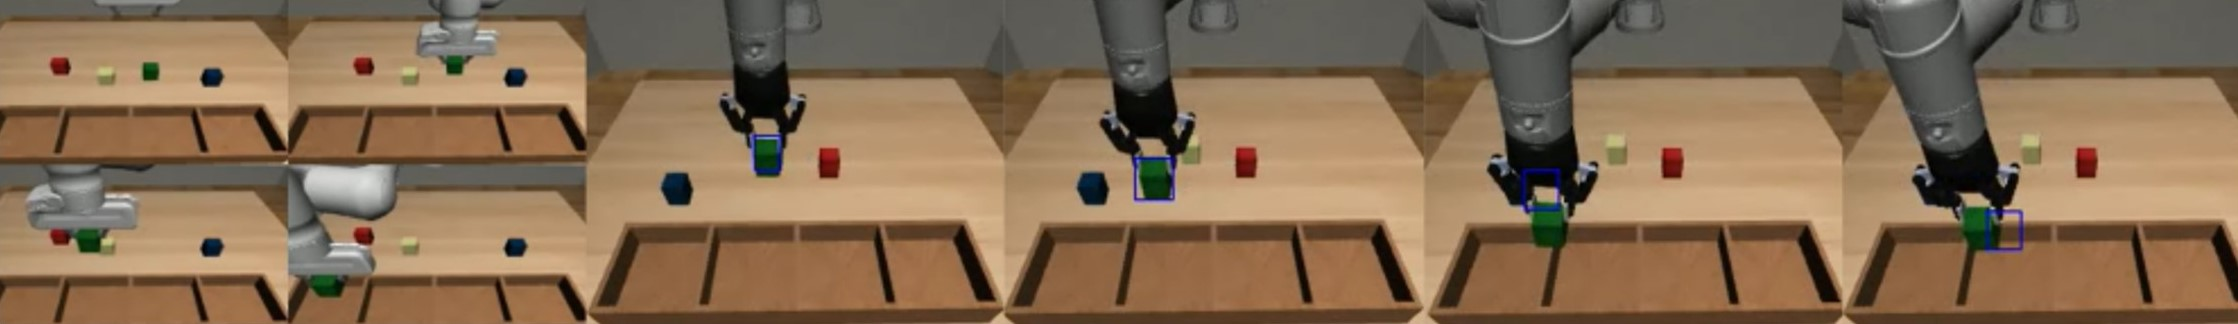
\includegraphics[width=1.0\textwidth]{figures/images/ch3/error_propagation.jpg}
    \caption{Example of unsuccessful Pick-Place rollout. In this case, the robot fails to complete the task due to errors in the bounding box predictions. These inaccuracies cause the robot to move in the wrong direction, leading to an unsuccessful execution of the task.}
    \label{fig:error_propagation}
\end{figure}


To address this issue, the Double-Control Module architecture has been proposed (Section \ref{sec:ocpl_architecture_dcm}), with the corresponding results presented in Section \ref{sec:ocpl_results_dcm}.

\paragraph*{Multi-task multi-variation scenario}\mbox{}\\
As in the previous paragraph, an evaluation of the two baseline methods was also conducted in the multi-task setting. The results are summarized in Table \ref{table:occp_multi_task_baseline_res}. The same general trends and behaviors observed in the single-task scenario are present here as well. Specifically, both baselines demonstrate the ability to produce reasonable trajectories that allow the robot to complete the task, though they manipulate the wrong object.

Furthermore, when comparing the results from Table \ref{table:occp_single_task_baseline_res} with those in Table \ref{table:occp_multi_task_baseline_res}, it is evident that the success rate decreases across all methods in the more complex multi-task setting. This highlights a potential issue with task balancing during the learning process.
% \usepackage{makecell}
% \usepackage{graphicx}
% \usepackage{multirow}
% \usepackage{hhline}


\begin{table}[t]
  \centering
  \caption{The multi-task performance of the baseline methods, TOSIL \cite{dasari2021transformers_one_shot} and MOSAIC \cite{mandi2022towards_more_generalizable_one_shot}, was evaluated. For each model, additional tests were conducted by generating the first 2 steps and 10 steps using the hand-written controller.}
  \label{table:occp_multi_task_baseline_res}
  \resizebox{\linewidth}{!}{%
  \begin{tabular}{|c|c|c|c|c|c|c|c|c|} 
  \hline
  \textbf{Task} & \textbf{Model} & \textbf{GT Action} & \begin{tabular}[c]{@{}c@{}}\textbf{Reaching}\\{[}\%]\end{tabular} & \begin{tabular}[c]{@{}c@{}}\textbf{Picking}\\{[}\%]\end{tabular} & \begin{tabular}[c]{@{}c@{}}\textbf{Success}\\{[}\%]\end{tabular} & \begin{tabular}[c]{@{}c@{}}\textbf{Reaching} \\\textbf{Wrong}~\\{[}\%]\end{tabular} & \begin{tabular}[c]{@{}c@{}}\textbf{Picking}\\\textbf{Wrong}\\{[}\%]\end{tabular} & \begin{tabular}[c]{@{}c@{}}\textbf{Success with}\\\textbf{Wrong Object}\\{[}\%]\end{tabular} \\ 
  \hhline{|=========|}
  \multirow{6}{*}{\rotatebox[origin=c]{90}{Pick-Place}} & \multirow{3}{*}{MOSAIC} & 0 & 25.83$\pm$1.30 & 23.96$\pm$0.72 & 22.71$\pm$0.72 & 65.63$\pm$2.87 & 63.96$\pm$1.90 & \textbf{67.92$\pm$1.30} \\ 
  \cline{3-9}
   &  & 2 & 61.04$\pm$2.19 & 58.13$\pm$2.86 & 56.46$\pm$3.14 & 36.04$\pm$1.90 & 35.42$\pm$1.90 & 36.25$\pm$1.08 \\ 
  \cline{3-9}
   &  & 10 & 97.77$\pm$0.36 & 95.00$\pm$0.62 & \textbf{87.50$\pm$1.25} & 2.50$\pm$0.62 & 2.29$\pm$0.95 & 2.29$\pm$0.72 \\ 
  \cline{2-9}
   & \multirow{3}{*}{TOSIL} & 0 & 35.42$\pm$0.72 & 27.08$\pm$1.30 & 26.46$\pm$1.80 & 60.21$\pm$1.57 & 59.58$\pm$1.44 & 59.58$\pm$1.44 \\ 
  \cline{3-9}
   &  & 2 &  &  &  &  &  &  \\ 
  \cline{3-9}
   &  & 10 &  &  &  &  &  &  \\ 
  \hhline{|=========|}
  \multirow{6}{*}{\rotatebox[origin=c]{90}{Stack-Block}} & \multirow{3}{*}{MOSAIC} & 0 & 32.96$\pm$1.28 & 30.74$\pm$2.31 & 28.53$\pm$2.31 & 56.30$\pm$4.49 & 48.15$\pm$4.20 & 41.67$\pm$1.66 \\ 
  \cline{3-9}
   &  & 2 & 76.67$\pm$1.11 & 73.33$\pm$1.92 & 65.56$\pm$4.00 & 19.63$\pm$0.64 & 17.41$\pm$1.28 & 17.04$\pm$1.69 \\ 
  \cline{3-9}
   &  & 10 & 100.00$\pm$0.00 & 97.78$\pm$1.11 & \textbf{82.96$\pm$1.28} & 0.00$\pm$0.00 & 0.00$\pm$0.00 & 0.00$\pm$0.00 \\ 
  \cline{2-9}
   & \multirow{3}{*}{TOSIL} & 0 & 27.78$\pm$2.94 & 24.44$\pm$2.94 & 22.59$\pm$3.57 & 70.37$\pm$2.57 & 67.78$\pm$2.22 & \textbf{64.81$\pm$2.57} \\ 
  \cline{3-9}
   &  & 2 &  &  &  &  &  &  \\ 
  \cline{3-9}
   &  & 10 &  &  &  &  &  &  \\ 
  \hhline{|=========|}
  \multirow{6}{*}{\rotatebox[origin=c]{90}{Nut-Assembly}} & \multirow{3}{*}{MOSAIC} & 0 & 57.78$\pm$1.92 & 57.78$\pm$1.92 & 55.56$\pm$2.54 & 42.22$\pm$1.92 & 42.22$\pm$1.93 & 41.11$\pm$1.67 \\ 
  \cline{3-9}
   &  & 2 & 95.56$\pm$0.96 & 95.56$\pm$0.96 & 89.44$\pm$1.92 & 4.44$\pm$0.96 & 4.44$\pm$0.96 & 4.44$\pm$0.96 \\ 
  \cline{3-9}
   &  & 10 & 100.00$\pm$0.00 & 100.00$\pm$0.00 & \textbf{92.22$\pm$0.96} & 0.00$\pm$0.00 & 0.00$\pm$0.00 & 0.00$\pm$0.00 \\ 
  \cline{2-9}
   & \multirow{3}{*}{TOSIL} & 0 & 54.44$\pm$0.96 & 54.44$\pm$0.96 & 48.89$\pm$0.96 & 46.11$\pm$0.96 & 45.56$\pm$0.96 & \textbf{45.56$\pm$0.96} \\ 
  \cline{3-9}
   &  & 2 &  &  &  &  &  &  \\ 
  \cline{3-9}
   &  & 10 &  &  &  &  &  &  \\ 
  \hhline{|=========|}
  \multirow{6}{*}{\rotatebox[origin=c]{90}{Press-Button}} & \multirow{3}{*}{MOSAIC} & 0 & 78.33$\pm$1.66 & - & 77.22$\pm$2.54 & 22.78$\pm$2.54 & - & 22.78$\pm$2.54 \\ 
  \cline{3-9}
   &  & 2 & 77.22$\pm$0.96 & - & 76.67$\pm$1.67 & 23.33$\pm$1.66 & - & 23.33$\pm$1.66 \\ 
  \cline{3-9}
   &  & 10 & 82.78$\pm$2.54 & - & \textbf{80.00$\pm$3.33} & 20.00$\pm$3.33 & - & 20.00$\pm$3.33 \\ 
  \cline{2-9}
   & \multirow{3}{*}{TOSIL} & 0 & 70.56$\pm$7.52 & - & 60.59$\pm$11.34 & 27.22$\pm$2.47 & - & \textbf{27.22$\pm$2.47} \\ 
  \cline{3-9}
   &  & 2 &  & - &  &  & - &  \\ 
  \cline{3-9}
   &  & 10 &  & - &  &  & - &  \\
  \hline
  \end{tabular}
  }
  \end{table}

After evaluating the baseline, the proposed MOSAIC-CTOD was tested, using the same variations as in the previous section. Table \ref{table:ctod_multi_task} summarizes the results obtained with the inclusion of positional information. Compared to the baseline, a general improvement is observed. However, caution is required when training the system in a multi-task setting. Specifically, when comparing the single-task performance (Table \ref{table:mosaic_ctod_single_task}) to the multi-task performance, there is a noticeable drop in success rates for the same tasks. This decline is particularly evident in the system's ability to execute the ``pick" primitive, especially when the nut object is involved. This observation underscores the importance of incorporating regularization techniques during multi-task learning to manage the varying complexities of different tasks.
% \usepackage{graphicx}
% \usepackage{multirow}
% \usepackage{hhline}


\begin{table}[t]
  \centering
  \caption{The multi-task performance of the proposed MOSAIC-CTOD module is compared to the MOSAIC and MOSAIC-GT-BB baselines. MOSAIC-GT-BB refers to the MOSAIC model, where the Control Module receives the ground-truth target bounding box as input.}
  \label{table:ctod_multi_task}
  \resizebox{\linewidth}{!}{%
  \begin{tabular}{|c|c|c|c|c|c|c|c|} 
  \hline
  \textbf{Task} & \textbf{Method} & \begin{tabular}[c]{@{}c@{}}\textbf{Reaching}\\{[}\%]\end{tabular} & \begin{tabular}[c]{@{}c@{}}\textbf{Picking}\\{[}\%]\end{tabular} & \begin{tabular}[c]{@{}c@{}}\textbf{Success}\\{[}\%]\end{tabular} & \begin{tabular}[c]{@{}c@{}}\textbf{Reaching }\\\textbf{Wrong~}\\{[}\%]\end{tabular} & \begin{tabular}[c]{@{}c@{}}\textbf{Picking}\\\textbf{Wrong}\\{[}\%]\end{tabular} & \begin{tabular}[c]{@{}c@{}}\textbf{Success with}\\\textbf{Wrong Object}\\{[}\%]\end{tabular} \\ 
  \hhline{|========|}
  \multirow{3}{*}{Pick-Place} & MOSAIC & 25.83$\pm$1.30 & 23.96$\pm$0.72 & 22.71$\pm$0.72 & 65.63$\pm$2.87 & 63.96$\pm$1.90 & 67.92$\pm$1.30 \\ 
  \cline{2-8}
   & MOSAIC-GT-BB & 100.00$\pm$0.00 & 89.58$\pm$2.19 & \textbf{58.33$\pm$0.90} & 0.00$\pm$0.00 & 0.00$\pm$0.00 & 0.00$\pm$0.00 \\ 
  \cline{2-8}
   & \begin{tabular}[c]{@{}c@{}}\textit{\textbf{MOSAIC-CTOD}}\\\textit{\textbf{(proposal)}}\end{tabular} & 80.21$\pm$1.44 & 67.50$\pm$0.62 & 53.33$\pm$1.90 & 4.16$\pm$0.71 & 3.54$\pm$0.36 & 0.37$\pm$0.64 \\ 
  \hhline{|========|}
  \multirow{3}{*}{Nut-Assembly} & MOSAIC & 32.96$\pm$1.28 & 30.74$\pm$2.31 & 28.53$\pm$2.31 & 56.30$\pm$4.49 & 48.15$\pm$4.20 & 41.67$\pm$1.66 \\ 
  \cline{2-8}
   & MOSAIC-GT-BB & 99.63$\pm$0.64 & 91.48$\pm$2.31 & \textbf{37.04$\pm$5.70} & 0.00$\pm$0.00 & 0.00$\pm$0.00 & 0.00$\pm$0.00 \\ 
  \cline{2-8}
   & \begin{tabular}[c]{@{}c@{}}\textit{\textbf{MOSAIC-CTOD}}\\\textit{\textbf{(proposal)}}\end{tabular} & 68.69$\pm$1.11 & 49.63$\pm$3.30 & 33.33$\pm$4.00 & 11.48$\pm$1.69 & 5.55$\pm$2.94 & 0.00$\pm$0.00 \\ 
  \hhline{|========|}
  \multirow{3}{*}{Stack-Block} & MOSAIC & 57.78$\pm$1.92 & 57.78$\pm$1.92 & 55.56$\pm$2.54 & 42.22$\pm$1.92 & 42.22$\pm$1.93 & 41.11$\pm$1.67 \\ 
  \cline{2-8}
   & MOSAIC-GT-BB & 94.44$\pm$5.85 & 91.11$\pm$6.73 & 73.89$\pm$5.00 & 10.00$\pm$2.88 & 0.00$\pm$0.00 & 0.00$\pm$0.00 \\ 
  \cline{2-8}
   & \begin{tabular}[c]{@{}c@{}}\textit{\textbf{MOSAIC-CTOD}}\\\textit{\textbf{(proposal)}}\end{tabular} & 97.92$\pm$2.09 & 96.67$\pm$2.35 & \textbf{87.92$\pm$2.00} & 1.25$\pm$0.83 & 0.41$\pm$0.83 & 0.00$\pm$0.00 \\ 
  \hhline{|========|}
  \multirow{3}{*}{Press-Button} & MOSAIC & 78.33$\pm$1.66 & - & 77.22$\pm$2.54 & 22.78$\pm$2.54 & - & 22.78$\pm$2.54 \\ 
  \cline{2-8}
   & MOSAIC-GT-BB & 100.00$\pm$0.00 & - & \textbf{98.33$\pm$0.00} & 0.55$\pm$0.96 & - & 0.55$\pm$0.96 \\ 
  \cline{2-8}
   & \begin{tabular}[c]{@{}c@{}}\textbf{\textit{MOSAIC-CTOD}}\\\textbf{\textit{(proposal)}}\end{tabular} & 92.78$\pm$0.96 & - & 91.11$\pm$2.54 & 3.89$\pm$4.19 & - & 3.88$\pm$4.19 \\
  \hline
  \end{tabular}
  }
  \end{table}

\subsubsection{Double control modules}
In this section the results obtained with the Double Control Module (Section \ref{sec:ocpl_architecture_dcm}) are going to be discussed.
\label{sec:ocpl_results_dcm}
\paragraph*{Single-task multi-variation scenario}\mbox{}\\
As discussed in Section \ref{sec:ocpl_architecture_dcm}, the introduction of the Double Control Module (DCM) was motivated by the need to reduce errors associated with incorrect object placement. These errors arise from inaccurate bounding-box predictions, which can lead to error propagation. 

To address this issue, the architecture of the Double Control Module evolved through incremental design iterations and validation steps.
Specifically, the process started by observing that the positional information given by the bouding-box is useful only during the reaching phase, while it becomes useless after it. For this reason, the training of the MOSAIC-CTOD has been changed, setting to zero the bounding-box after the picking. Then, observing the obtained results and the error cases, the Double Control Module has been realized.

% \usepackage{graphicx}
% \usepackage{multirow}
% \usepackage{hhline}


\begin{table}[t]
  \centering
  \caption{MOSAIC-COD results obtained in the single-task setting. The model is compared to baselines such as MOSAIC-CTOD (Section \ref{sec:ocpl_results_scm}), a modified version of MOSAIC-CTOD that does not receive the predicted bounding box after picking, and MOSAIC-DP, which is the MOSAIC architecture proposed in \cite{mandi2022towards_more_generalizable_one_shot}, but with two control modules.}
  \label{table:double_policy_single_task}
  \resizebox{\linewidth}{!}{%
  \begin{tabular}{|c|c|c|c|c|c|} 
  \hline
  \textbf{Task} & \textbf{Model} & \begin{tabular}[c]{@{}c@{}}\textbf{Reaching}\\{[}\%]\end{tabular} & \begin{tabular}[c]{@{}c@{}}\textbf{Picking}\\{[}\%]\end{tabular} & \begin{tabular}[c]{@{}c@{}}\textbf{Success}\\{[}\%]\end{tabular} & \begin{tabular}[c]{@{}c@{}}\textbf{Place Wrong}\\\textbf{Correct Object}\\{[}\%]\end{tabular} \\ 
  \hhline{|======|}
  \multirow{4}{*}{\vspace{-30px}\rotatebox[origin=c]{90}{Pick-Place}} & \begin{tabular}[c]{@{}c@{}}\textbf{\textit{MOSAIC-CTOD}}\\\textbf{\textit{(proposal)}}\end{tabular} & 98.12$\pm$0.62 & 91.88$\pm$4.88 & 77.11$\pm$5.60 & \textbf{11.25$\pm$1.08} \\ 
  \cline{2-6}
   & \begin{tabular}[c]{@{}c@{}}MOSAIC-CTOD\\(no-bb after pick)\end{tabular} & 95.69$\pm$1.88 & 83.89$\pm$3.45 & 82.36$\pm$3.13 & 0.00$\pm$0.00 \\ 
  \cline{2-6}
   & MOSAIC-DP & 36.60$\pm$0.32 & 28.82$\pm$1.26 & 27.36$\pm$1.59 & 0.00$\pm$0.00 \\ 
  \cline{2-6}
   & \begin{tabular}[c]{@{}c@{}}\textbf{\textit{MOSAIC-COD}}\\\textbf{\textit{(proposal)}}\end{tabular} & 100.00$\pm$0.00 & 93.75$\pm$0.62 & \textbf{93.33$\pm$0.72} & 0.00$\pm$0.00 \\ 
  \hhline{|======|}
  \multirow{4}{*}{\vspace{-30px}\rotatebox[origin=c]{90}{Nut-Assembly}} & \begin{tabular}[c]{@{}c@{}}\textbf{\textit{MOSAIC-CTOD}}\\\textbf{\textit{(proposal)}}\end{tabular} & 98.89$\pm$1.11 & 97.41$\pm$2.31 & 64.07$\pm$0.64 & \textbf{22.22$\pm$2.93} \\ 
  \cline{2-6}
   & \begin{tabular}[c]{@{}c@{}}MOSAIC-CTOD\\(no-bb after pick)\end{tabular} & 81.76$\pm$0.58 & 64.44$\pm$5.09 & 58.15$\pm$0.15 & 0.00$\pm$0.00 \\ 
  \cline{2-6}
   & MOSAIC-DP & 30.62$\pm$0.57 & 25.06$\pm$0.57 & 23.21$\pm$1.13 & 0.00$\pm$0.00 \\ 
  \cline{2-6}
   & \begin{tabular}[c]{@{}c@{}}\textbf{\textit{MOSAIC-COD}}\\\textbf{\textit{~ (proposal)}}\textit{}\end{tabular} & 99.63$\pm$0.64 & 85.19$\pm$4.60 & \textbf{81.11$\pm$3.84} & 0.00$\pm$0.00 \\ 
  \hhline{|======|}
  \multirow{4}{*}{\vspace{-30px}\rotatebox[origin=c]{90}{Stack-Block}} & \begin{tabular}[c]{@{}c@{}}\textbf{\textit{MOSAIC-CTOD}}\\\textbf{\textit{~ (proposal)}}\end{tabular} & 100.00$\pm$0.00 & 100.00$\pm$0.00 & 91.67$\pm$2.88 & - \\ 
  \cline{2-6}
   & \begin{tabular}[c]{@{}c@{}}MOSAIC-CTOD\\(no-bb after pick)\end{tabular} & 92.59$\pm$2.51 & 85.74$\pm$0.85 & 76.30$\pm$5.04 & - \\ 
  \cline{2-6}
   & MOSAIC-DP & 67.22$\pm$2.55 & 54.26$\pm$0.85 & 51.48$\pm$1.70 & - \\ 
  \cline{2-6}
   & \begin{tabular}[c]{@{}c@{}}\textbf{\textit{MOSAIC-COD}}\\\textbf{\textit{~ (proposal)}}\textit{}\end{tabular} & 100.00$\pm$0.00 & 100.00$\pm$0.00 & \textbf{95.00$\pm$1.66} & - \\ 
  \hhline{|======|}
  \multirow{4}{*}{\vspace{-30px}\rotatebox[origin=c]{90}{Press-Button}} & \begin{tabular}[c]{@{}c@{}}\textbf{\textit{MOSAIC-CTOD}}\\\textbf{\textit{~ (proposal)}}\end{tabular} & 97.22$\pm$1.92 & - & \textbf{95.56$\pm$1.92} & - \\ 
  \cline{2-6}
   & \begin{tabular}[c]{@{}c@{}}MOSAIC-CTOD\\(no-bb after pick)\end{tabular} & 81.85$\pm$3.35 & - & 77.04$\pm$3.39 & - \\ 
  \cline{2-6}
   & MOSAIC-DP & 88.70$\pm$3.39 &  & 82.96$\pm$5.89 & - \\ 
  \cline{2-6}
   & \begin{tabular}[c]{@{}c@{}}\textbf{\textit{MOSAIC-COD}}\\\textbf{\textit{~ (proposal)}}\textit{}\end{tabular} & 100.00$\pm$0.00 & - & 91.11$\pm$1.92 & - \\
  \hline
  \end{tabular}
  }
  \end{table}
Table \ref{table:double_policy_single_task} summarizes the obtained results, from which several important considerations can be made.

Firstly, it is noteworthy that removing the bounding box after picking reduces the error percentage for the \textit{Place Wrong Correct Object} category to 0.00\%, confirming the earlier observation regarding the noisy nature of the predicted bounding box after the picking phase. However, this modification alone does not lead to a general improvement in the overall success rate. In fact, the \textit{MOSAIC-CTOD (no-bb after pick)} model has a lower picking rate. This occurs because the control module issues the closing command too early, creating an out-of-distribution sample, which drives the robot into a novel state that was not encountered during training, making it unable to complete the task (Figure \ref{fig:error_no_bb_after_pick}).

\begin{figure}[t]
    \centering
    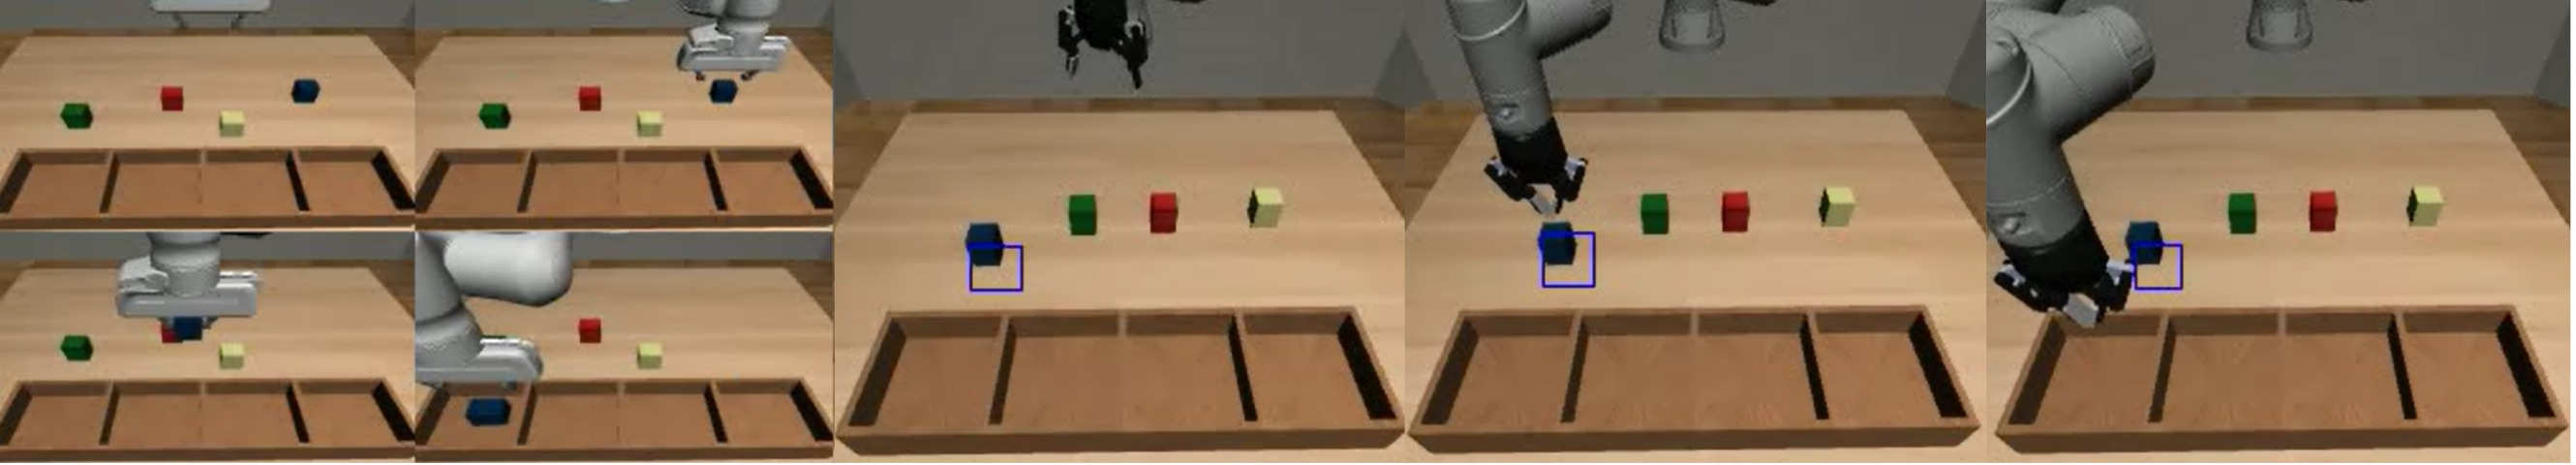
\includegraphics[width=1.0\textwidth]{figures/images/ch3/error_no_bb_after_pick.jpg}
    \caption{Example of an unsuccessful Pick-Place operation using the  ``no-bb after pick" variant. In this scenario, the robot successfully reaches the target box based on the predicted bounding box (blue). However, the single-control module prematurely predicts the closing command, preventing the robot from correctly picking up the object.}
    \label{fig:error_no_bb_after_pick}
\end{figure}

% \smalltodo{add figure}

Regarding the performance of the proposed \textit{MOSAIC-COD} module, it is notable that it achieves the highest success rate in 3 out of 4 tasks. Specifically, for tasks prone to placing the correct object in the wrong position, such as Pick-Place and Nut-Assembly, this type of error is eliminated, resulting in an overall improvement in the success rate.

Additionally, a novel variant of the MOSAIC baseline, \\ \textit{MOSAIC-DP}, has been implemented. This model follows the classic MOSAIC architecture proposed in \cite{mandi2022towards_more_generalizable_one_shot}, but it is equipped with two control modules. One module handles the reaching primitive, while the other is responsible for the primitive used in the final part of the task (i.e., placing, assembly, stacking, or pushing, respectively).

It is important to note that the performance of this variation is very similar to the original MOSAIC baseline, even though the control problem is simplified by splitting it into two phases corresponding to different primitives. Specifically, the most significant error in this case also stems from manipulating the wrong object. The success rates with the wrong object are 54.38\%, 46.67\%, 46.67\%, and 7.59\% for the Pick-Place, Nut-Assembly, Stack-Block, and Press-Button tasks, respectively. 

This further supports the central thesis, which suggests that the end-to-end architecture struggles to create an optimal embedding that addresses both cognitive and control tasks effectively.

\paragraph*{Multi-task multi-variation scenario}\mbox{}\\
\begin{table}[t]
  \scriptsize
  \selectfont
  \centering
  \refstepcounter{table}
  \caption{MOSAIC-COD results obtained in the multi-task setting. The model is compared with MOSAIC and MOSAIC-CTOD models.}
  \label{table:double_policy_multi_task}
  \resizebox{\linewidth}{!}{%
  \begin{tabular}{|c|c|c|c|c|} 
  \hline
  \textbf{Task} & \textbf{Model} & \begin{tabular}[c]{@{}c@{}}\textbf{Reaching}\\{[}\%]\end{tabular} &  \begin{tabular}[c]{@{}c@{}}\textbf{Picking}\\{[}\%]\end{tabular} & \begin{tabular}[c]{@{}c@{}}\textbf{Success}\\{[}\%]\end{tabular} \\ 
  \hhline{|=====|}
  \multirow{3}{*}{Pick-Place} & MOSAIC & 25.83$\pm$1.30 & 23.96$\pm$0.72 & 22.71$\pm$0.72 \\ 
  \cline{2-5}
   & MOSAIC-CTOD & 80.21$\pm$1.44 & 67.50$\pm$0.62 & 53.33$\pm$1.90 \\ 
  \cline{2-5}
   & \textit{MOSAIC-COD} & 100.00$\pm$0.00 & 94.79$\pm$0.90 & \textbf{89.58$\pm$3.55} \\ 
  \hhline{|=====|}
  \multirow{3}{*}{Nut-Assembly} & MOSAIC & 32.96$\pm$1.28 & 30.74$\pm$2.31 & 28.53$\pm$2.31 \\ 
  \cline{2-5}
   & MOSAIC-CTOD & 68.69$\pm$1.11 & 49.63$\pm$3.30 & 33.33$\pm$4.00 \\ 
  \cline{2-5}
   & \textit{MOSAIC-COD} & 99.63$\pm$0.64 & 78.15$\pm$2.31 & \textbf{70.74$\pm$4.49} \\ 
  \hhline{|=====|}
  \multirow{3}{*}{Stack-Block} & MOSAIC & 57.78$\pm$1.92 & 57.78$\pm$1.92 & 55.56$\pm$2.54 \\ 
  \cline{2-5}
   & MOSAIC-CTOD & 97.92$\pm$2.09 & 96.67$\pm$2.35 & \textbf{87.92$\pm$2.00} \\ 
  \cline{2-5}
   & \textit{MOSAIC-COD} & 98.33$\pm$0.00 & 98.33$\pm$0.00 & 85.00$\pm$5.00 \\ 
  \hhline{|=====|}
  \multirow{3}{*}{Press-Button} & MOSAIC & 78.33$\pm$1.66 & - & 77.22$\pm$2.54 \\ 
  \cline{2-5}
   & MOSAIC-CTOD & 92.78$\pm$0.96 & - & \textbf{91.11$\pm$2.54} \\ 
  \cline{2-5}
   & \textit{MOSAIC-COD} & 83.89$\pm$2.55 & - & 71.67$\pm$2.88 \\
  \hline
  \end{tabular}
  }
  \end{table}
Given the results and observations from the previous section, the MOSAIC-COD module is directly compared to the baselines MOSAIC and MOSAIC-CTOD in the Multi-Task setting. Table \ref{table:cod_multi_task_performance} summarizes the results. As can be seen, the use of specialized models trained for the two task phases, reaching and placing, leads to a system that consistently picks the target object. This improvement is particularly evident in the more complex tasks, such as Pick-Place and Nut-Assembly. The enhanced picking rate demonstrates that having accurate information about the target object position enables correct target acquisition, while the presence of two control modules allows for training specific controllers for simpler primitives.

However, despite the improvements observed in Pick-Place and Nut-Assembly, MOSAIC-COD has the lowest overall success rate on the Press-Button task. This can be attributed to two main factors. First, the Press-Button task is substantially different from the other three tasks. Unlike the others, it does not involve pick-and-place primitives, making it an out-of-distribution task. Second, the instability of the bounding boxes produced can lead to undesirable behaviors, such as sudden movements or freezing.
% \smalltodo{add figure}

\subsubsection{Proprioceptive state and Generalization tests}
\begin{figure}[t]
    \centering
    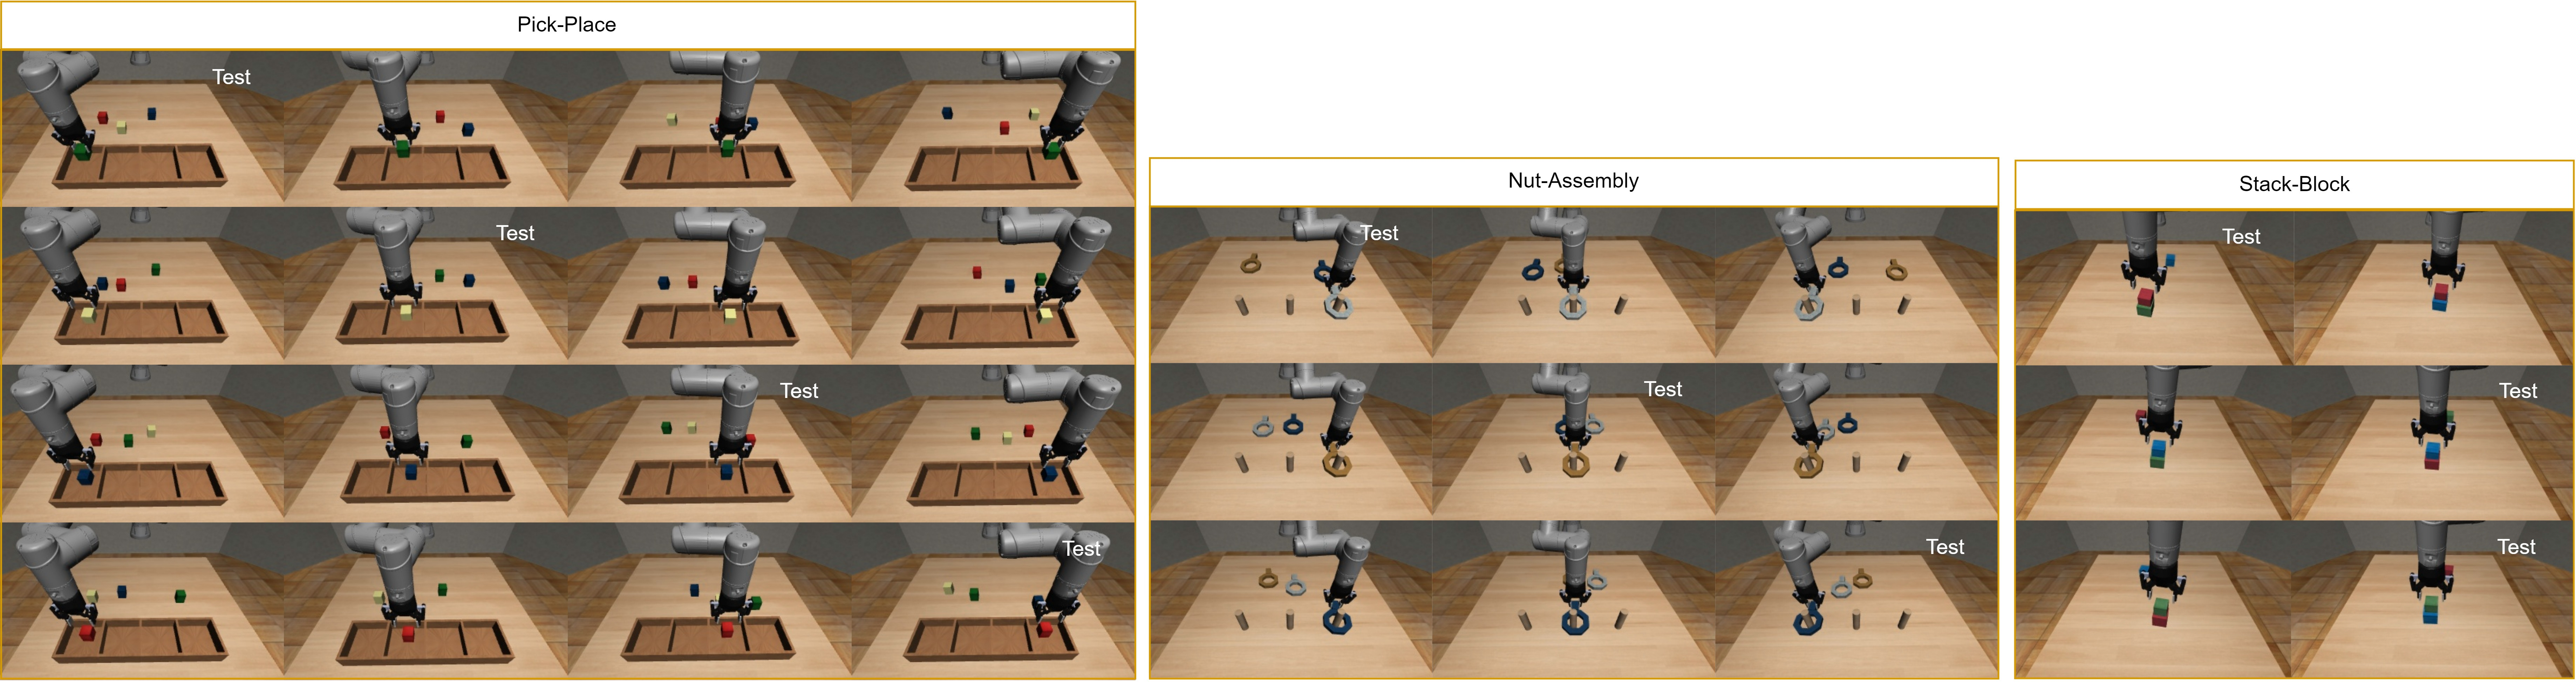
\includegraphics[width=1.0\textwidth]{figures/images/ch3/generalization_dataset.jpg}
    \caption{The dataset used for generalization tests removes one variation from each set of variations for a given target object.}
    \label{fig:generalization_dataset}
\end{figure}


\begin{figure}[t]
    \centering
    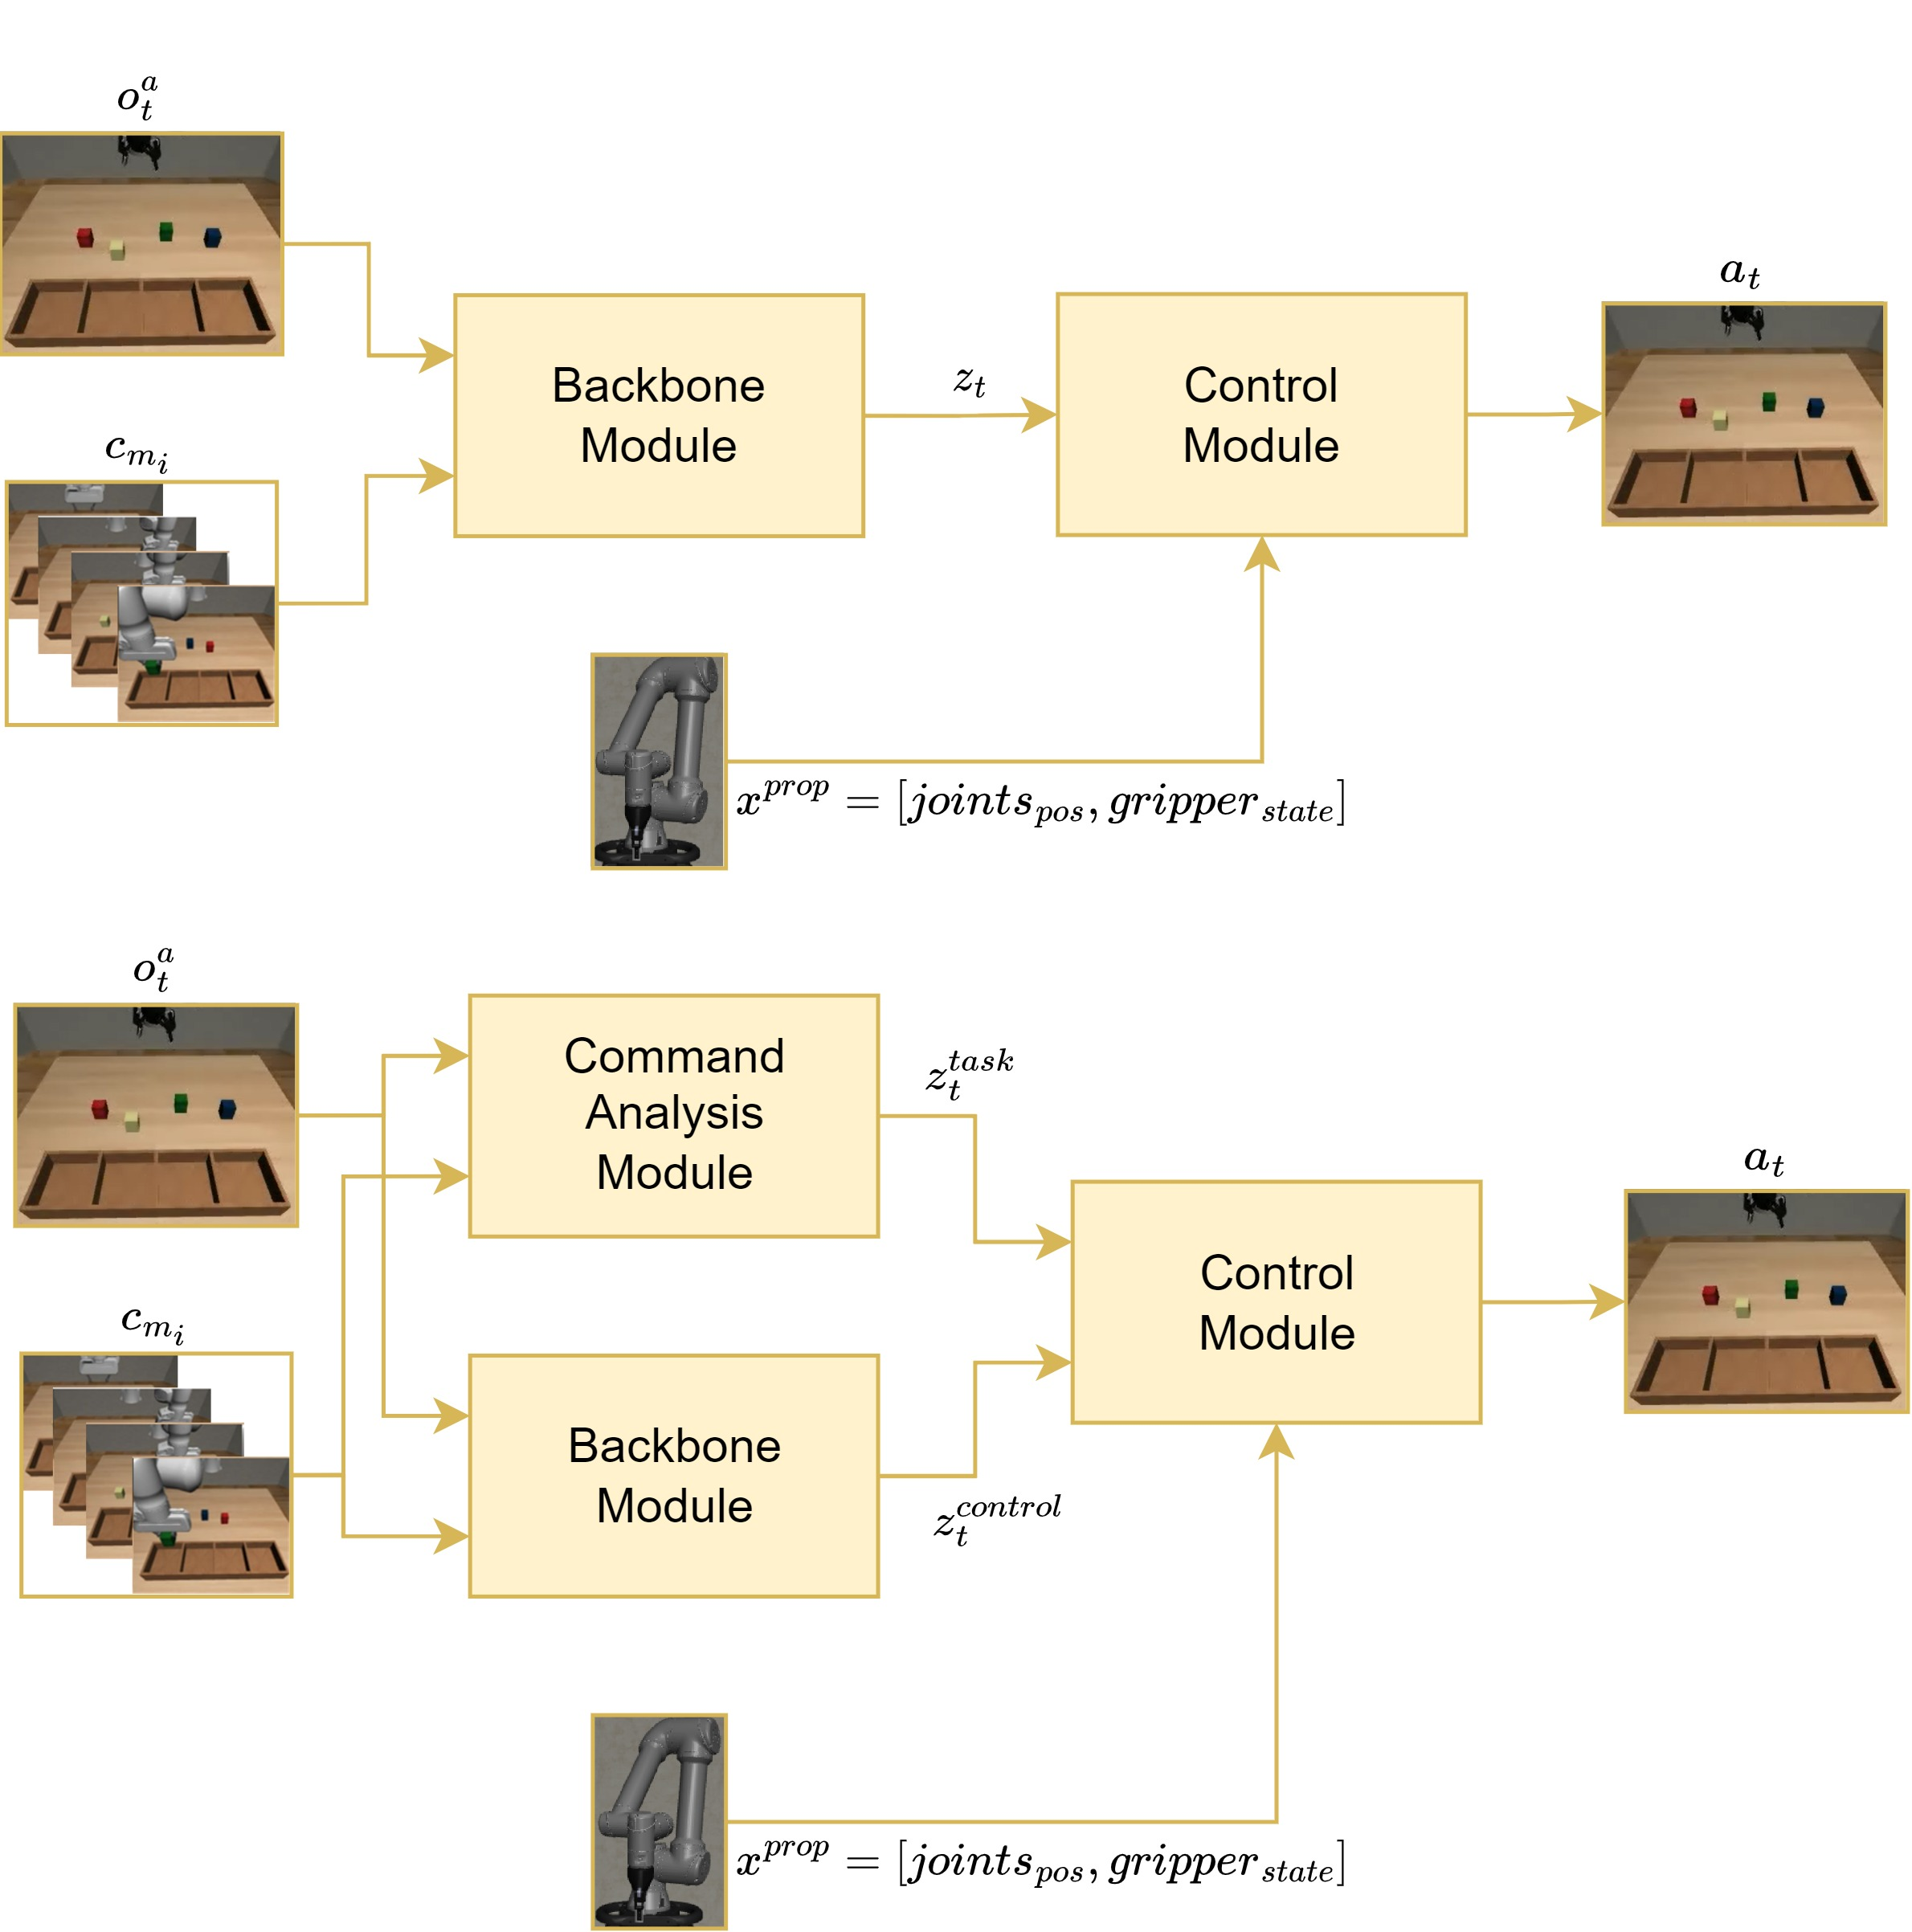
\includegraphics[width=0.7\textwidth]{figures/images/ch3/end_to_end_vs_modular_proprioceptive.jpg}
    \caption{Proprioceptive information is integrated in both the end-to-end architecture (top) and the modular architecture (bottom). The proprioceptive vector, $x^{prop}$, is constructed from the robot's six continuous joint positions and the binary gripper state.}
    \label{fig:end_to_end_vs_modular_proprioceptive}
\end{figure}

In this section, additional experiments are described, focusing on two key objectives.

The first set of experiments aims to determine whether the integration of proprioceptive information can enhance the system's robustness. This is particularly important for tasks requiring fine manipulation, such as the Nut-Assembly task, where the goal is to reduce errors during the assembly phase, specifically avoiding instances where the nut hits the peg.

The second set of experiments explores the generalization capabilities of the proposed system. Specifically, the goal is to assess whether the system can generalize to previously unseen task variations. To evaluate this, the system is trained on a subset of task variations selected as follows: for a set of variations involving a specific target object (e.g., a green box), one variation is excluded (e.g., placing the box into the first bin). However, in other sets involving different objects, the variation that requires placing the object into the first bin is retained. This setup allows for testing how well the system can transfer knowledge across different variations. By doing so, it becomes possible to evaluate whether the system can achieve robust performance with less training data, eliminating the need to collect every possible variation for each object (Figure \ref{fig:generalization_dataset}).
% \smalltodo{add figure}

\begin{table}[t]
  \centering
  \caption{The results obtained by integrating proprioceptive information in both Single-Task and Multi-Task scenarios. For each baseline model, MOSAIC, MOSAIC-CTOD, and MOSAIC-COD, the corresponding version that includes the proprioceptive state (P) was trained and tested.}
  \label{table:proprioceptive}
  \resizebox{\linewidth}{!}{%
  \begin{tabular}{|c|c|c|c|} 
  \hline
  \textbf{Task} & \textbf{Model} & \begin{tabular}[c]{@{}c@{}}\textbf{Success}\\\textbf{(Single-Task)}\\{[}\%]\end{tabular} & \begin{tabular}[c]{@{}c@{}}\textbf{Success}\\\textbf{(Multi-Task)}\\{[}\%]\end{tabular} \\ 
  \hhline{|====|}
  \multirow{6}{*}{Pick-Place} & MOSAIC & 58.75$\pm$1.87 &  \\ 
  \cline{2-4}
   & \textit{MOSAIC-P} & 12.84$\pm$0.31 &  \\ 
  \cline{2-4}
   & MOSAIC-CTOD & 77.11$\pm$5.60 &  \\ 
  \cline{2-4}
   & \textit{MOSAIC-CTOD-P} & 87.84$\pm$2.43 &  \\ 
  \cline{2-4}
   & MOSAIC-COD & 93.33$\pm$0.72 &  \\ 
  \cline{2-4}
   & \textit{MOSAIC-COD-P} & \textbf{96.04$\pm$0.56} &  \\ 
  \hhline{|====|}
  \multirow{6}{*}{Nut-Assembly} & MOSAIC & 33.33$\pm$1.11 &  \\ 
  \cline{2-4}
   & \textit{MOSAIC-P} & 13.83$\pm$0.57 &  \\ 
  \cline{2-4}
   & MOSAIC-CTOD & 64.07$\pm$0.64 &  \\ 
  \cline{2-4}
   & \textit{MOSAIC-CTOD-P} & 95.06$\pm$0.56 &  \\ 
  \cline{2-4}
   & MOSAIC-COD & 81.11$\pm$3.84 &  \\ 
  \cline{2-4}
   & \textit{MOSAIC-COD-P} & \textbf{95.06$\pm$0.57} &  \\ 
  \hhline{|====|}
  \multirow{6}{*}{Stack-Block} & MOSAIC & 53.33$\pm$1.66 &  \\ 
  \cline{2-4}
   & \textit{MOSAIC-P} & 29.07$\pm$2.50 &  \\ 
  \cline{2-4}
   & MOSAIC-CTOD & 91.67$\pm$2.88 &  \\ 
  \cline{2-4}
   & \textit{MOSAIC-CTOD-P} & 91.11$\pm$6.90 &  \\ 
  \cline{2-4}
   & \textit{MOSAIC-COD} & 95.00$\pm$1.66 &  \\ 
  \cline{2-4}
   & \textit{MOSAIC-COD-P} & \textbf{96.67$\pm$1.66} &  \\ 
  \hhline{|====|}
  \multirow{6}{*}{Press-Button} & MOSAIC & \textbf{100.00$\pm$0.00} &  \\ 
  \cline{2-4}
   & \textit{MOSAIC-P} & 65.00$\pm$3.33 &  \\ 
  \cline{2-4}
   & MOSAIC-CTOD & 95.56$\pm$1.92 &  \\ 
  \cline{2-4}
   & \textit{MOSAIC-CTOD-P} & 86.66$\pm$6.66 &  \\ 
  \cline{2-4}
   & MOSAIC-COD & 91.11$\pm$1.92 &  \\ 
  \cline{2-4}
   & \textit{MOSAIC-COD-P} & 72.03$\pm$3.39 &  \\
  \hline
  \end{tabular}
  }
  \end{table}
\paragraph*{Proprioceptive information}\mbox{}\\
The proprioceptive information selected for the four tasks considered includes the joint positions, $joints_{pos} \in \mathcal{R}^{6}$ and the gripper state, $gripper_{state} \in \left[ 0, 1 \right]$. This vector of elements, $x^{prop}$, is provided as input directly to the Control Module, as shown in Figure \ref{fig:end_to_end_vs_modular_proprioceptive}. 
% \smalltodo{add figure}

Specifically, for each baseline method, \textit{MOSAIC}, \textit{MOSAIC-CTOD}, and \textit{MOSAIC-COD}, a version of the model incorporating proprioceptive information was trained. Table \ref{table:proprioceptive} presents the success rates for both the Single-Task and Multi-Task scenarios. 

It is important to note that for 3 out of 4 tasks, the best performance is achieved by combining the Double-Policy approach with proprioceptive information, effectively solving the manipulation tasks of Pick-Place, Nut-Assembly, and Stack-Block in a robust manner. The greatest improvement is seen in the Nut-Assembly task, where the proprioceptive information resolves issues related to collisions and robot freezing.

However, this improvement is not observed in the Press-Button task, where a 35\% drop in success rate is seen, even with the \textit{MOSAIC} baseline. In this task, the main failure cases are related to unstable robot behavior. Additionally, in variations focused on object orientation, the robot often gets stuck when correctly approaching the button.

Notably, this behavior is not observed in the Multi-Task scenario. In fact, the highest performance is achieved by methods that exclude proprioceptive information. Interestingly, the inclusion of proprioceptive data seems to exacerbate the imbalance between tasks, preventing the system from effectively leveraging this additional information during testing and resulting in instability.

For example, in the case of the MOSAIC-CTOD-P module, the robot successfully picks the target object only 58.87\% of the time. This occurs because the closing command is sent too early, relative to the object position. Furthermore, the success rate drops further to 38.14\%, as the robot, despite reaching the target peg, collides with it, an issue where proprioceptive information should theoretically provide assistance, especially since the pegs are fixed.

This instability is most evident in the Stack-Block task, where the success rate falls to 22.77\% for the MOSAIC-COD-P module, despite the robot picking the target object with an average rate of 80.00\%. The errors in this case are due to the object being dropped during stacking, caused by imprecise placement, as well as instances where the robot becomes completely stuck.

These results highlight the need for a balanced learning procedure in the context of Multi-Task Learning, as discussed earlier in Section \ref{sec:ocpl_results_scm}.

% \usepackage{graphicx}
% \usepackage{multirow}
% \usepackage{hhline}


\begin{table}[t]
  \centering
  \caption{The results obtained by testing the models on unseen variations.}
  \label{table:generalization}
  \resizebox{\linewidth}{!}{%
  \begin{tabular}{|c|c|c|c|c|c|} 
  \hline
  \textbf{Task} & \textbf{Model} & \begin{tabular}[c]{@{}c@{}}\textbf{Reaching}\\\textbf{(Single-Task)}\\{[}\%]\end{tabular} & \begin{tabular}[c]{@{}c@{}}\textbf{Success}\\\textbf{(Single-Task)}\\{[}\%]\end{tabular} & \begin{tabular}[c]{@{}c@{}}\textbf{Reaching}\\\textbf{(Multi-Task)}\\{[}\%]\end{tabular} & \begin{tabular}[c]{@{}c@{}}\textbf{Success}\\\textbf{(Multi-Task)}\\\textbf{\textbf{}}\%]\end{tabular} \\ 
  \hhline{|======|}
  \multirow{3}{*}{\vspace{-30px}\rotatebox[origin=c]{90}{Pick-Place}} & MOSAIC & 35.83$\pm$2.82 & 31.67$\pm$3.82 & 32.50$\pm$2.50 & 20.83$\pm$5.70 \\ 
  \cline{2-6}
   & \begin{tabular}[c]{@{}c@{}}\textbf{\textit{MOSAIC-CTOD}}\\\textbf{\textit{(proposal)}}\end{tabular} & 100.00$\pm$0.00 & 87.50$\pm$4.30 & 100.00$\pm$0.00 & 63.33$\pm$5.20 \\ 
  \cline{2-6}
   & \begin{tabular}[c]{@{}c@{}}\textbf{\textit{MOSAIC-COD}}\\\textbf{\textit{(proposal)}}\end{tabular} & 100.00$\pm$0.00 & \textbf{89.17$\pm$2.89} & 100.00$\pm$0.00 & \textbf{94.17$\pm$2.88} \\ 
  \hhline{|======|}
  \multirow{3}{*}{\vspace{-30px}\rotatebox[origin=c]{90}{Nut-Assembly}} & MOSAIC & 22.22$\pm$1.93 & 13.33$\pm$3.33 & 27.78$\pm$3.85 & 18.88$\pm$3.84 \\ 
  \cline{2-6}
   & \begin{tabular}[c]{@{}c@{}}\textbf{\textit{MOSAIC-CTOD}}\\\textbf{\textit{(proposal)}}\end{tabular} & 100.00$\pm$0.00 & 38.89$\pm$6.94 & 100.00$\pm$0.00 & 51.11$\pm$1.92 \\ 
  \cline{2-6}
   & \begin{tabular}[c]{@{}c@{}}\textbf{\textit{MOSAIC-COD}}\\\textbf{\textit{(proposal)}}\end{tabular} & 98.89$\pm$1.93 & \textbf{57.78$\pm$5.09} & 100.00$\pm$0.00 & \textbf{90.00$\pm$3.33} \\ 
  \hhline{|======|}
  \multirow{3}{*}{\vspace{-30px}\rotatebox[origin=c]{90}{Stack-Block}} & MOSAIC & 58.89$\pm$1.93 & 53.33$\pm$3.33 & 60.00$\pm$5.77 & 56.66$\pm$3.33 \\ 
  \cline{2-6}
   & \begin{tabular}[c]{@{}c@{}}\textbf{\textit{MOSAIC-CTOD}}\\\textbf{\textit{(proposal)}}\end{tabular} & 100.00$\pm$0.00 & 94.44$\pm$6.94 & 100.00$\pm$0.00 & \textbf{88.88$\pm$5.00} \\ 
  \cline{2-6}
   & \begin{tabular}[c]{@{}c@{}}\textbf{\textit{MOSAIC-COD}}\\\textbf{\textit{(proposal)}}\end{tabular} & 100.00$\pm$0.00 & \textbf{97.78$\pm$1.93} & 100.00$\pm$0.00 & 72.20$\pm$5.09 \\
  \hline
  \end{tabular}
  }
  \end{table}
\paragraph*{Generalization}\mbox{}\\
Regarding the generalization tests, we evaluated only the three tasks where the previously explained variation selection was applicable. Specifically, the following variations were removed for each task (Figure \ref{fig:generalization_dataset}):

\begin{itemize}
    \item \textbf{Pick-Place}: Variations 1, 6, 11, and 16 were excluded.
    \item \textbf{Nut-Assembly}: Variations 1, 5, and 9 were excluded.
    \item \textbf{Stack-Block}: Variations 1, 4, and 6 were excluded.
\end{itemize}

The models were trained on the remaining variations and tested on the excluded ones following the same procedure.

Table \ref{table:generalization} summarizes the success rates obtained for both the Single-Task and Multi-Task settings. Notably, with the introduction of the CTOD and COD modules, the system consistently reaches the correct target object in unseen variations. Similarly, the robot is able to pick and complete tasks, outperforming the MOSAIC baseline across all tested tasks.

This is a promising result, as it demonstrates that the system can effectively share knowledge across different variations, enabling robust training with fewer data.



\chapter{Experimental validation in real-world scenario}
\label{ch:real_world_application}
This chapter details the validation of the proposed methods in a real world scenario. Specifically, Section~\ref{sec:real_world_exp_setting} describes the experimental setup. Section~\ref{sec:real_world_dataset} discusses the dataset used to train the system. Finally, Section~\ref{sec:real_results} presents the results obtained.

\section{Experimental Setting}
\label{sec:real_world_exp_setting}
In this section, the experimental setup is explained and defined. Figure \ref{fig:workspace} illustrates the workspace where the robot operates, and compares it to the corresponding simulation environment. As can be observed, the simulation environment closely resembles the real-world counterpart. Both environments consist of the same robot agent, with identical camera configurations and workspace setup.

\begin{figure}[t]
    \centering
    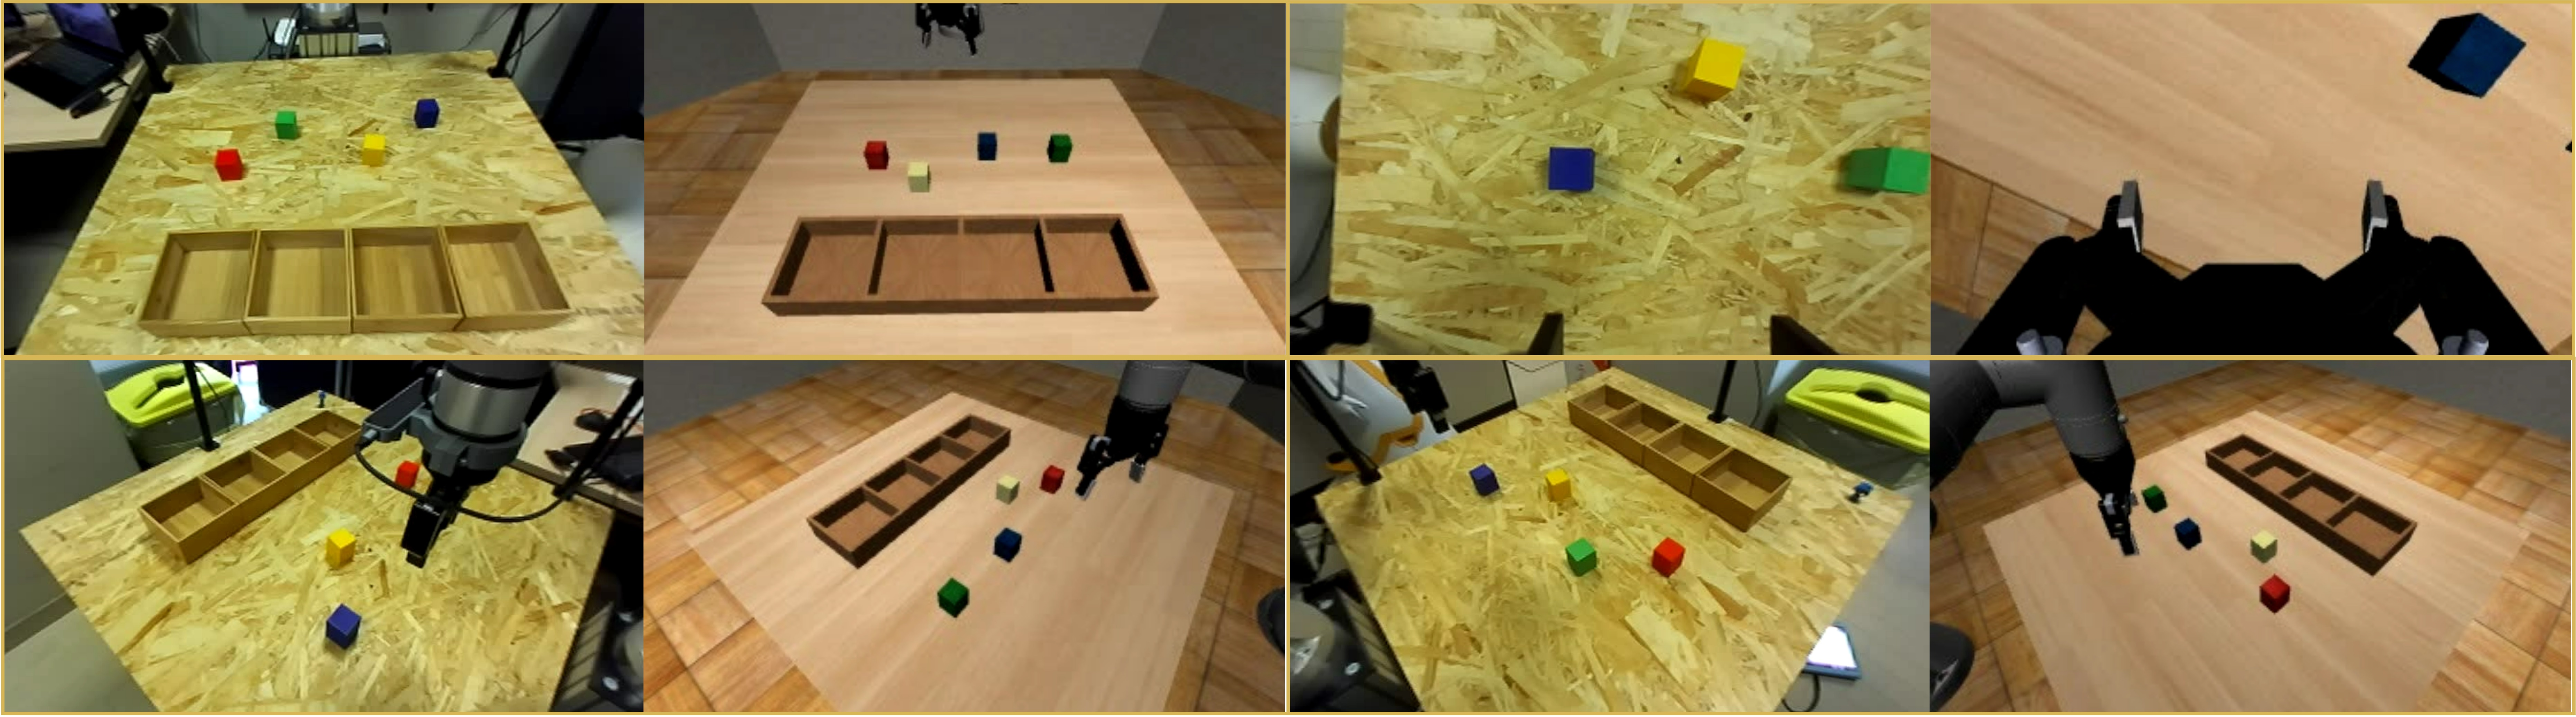
\includegraphics[width=1.0\textwidth]{figures/images/ch5/workspace.jpg}
    \caption{Workspace comparison between real-world (left) and simulated (right) scenarios. Images are taken from the frontal camera (Top-Left), the gripper camera (Top-Right), lateral-left camera (Bottom-Left) and lateral-right (Bottom-Right).}
    \label{fig:workspace}
\end{figure}

Specifically, the experimental setup includes:
\begin{itemize}
    \item The Universal Robots UR5e robot \cite{ur5e}, equipped with the Robotiq 2F-85 gripper \cite{robotiq}, which acts as the agent.
    \item Four Zed-Mini stereo cameras \cite{zed}, one camera is mounted on the gripper, while the remaining three are positioned around the robot to ensure complete coverage of the workspace.
    \item A 100$\times$100 cm working table.
\end{itemize}

The reason for maintaining a high similarity between the real-world and simulation environments is to evaluate the potential for pre-training the model on a large and comprehensive simulation dataset, followed by fine-tuning on a smaller and incomplete real-world dataset. This approach allows leveraging the advantages of simulation for initial training while adapting the model to real-world conditions with minimal additional data.

\section{Dataset}
\label{sec:real_world_dataset}
For the real-world validation, the focus will be on testing the model on the \textbf{multi-variation} \textit{Pick-Place} tasks, focusing on a smaller set of variations compared to the complete 16 variations described in Section \ref{sec:cod_dataset}.

\begin{figure}[t]
    \centering
    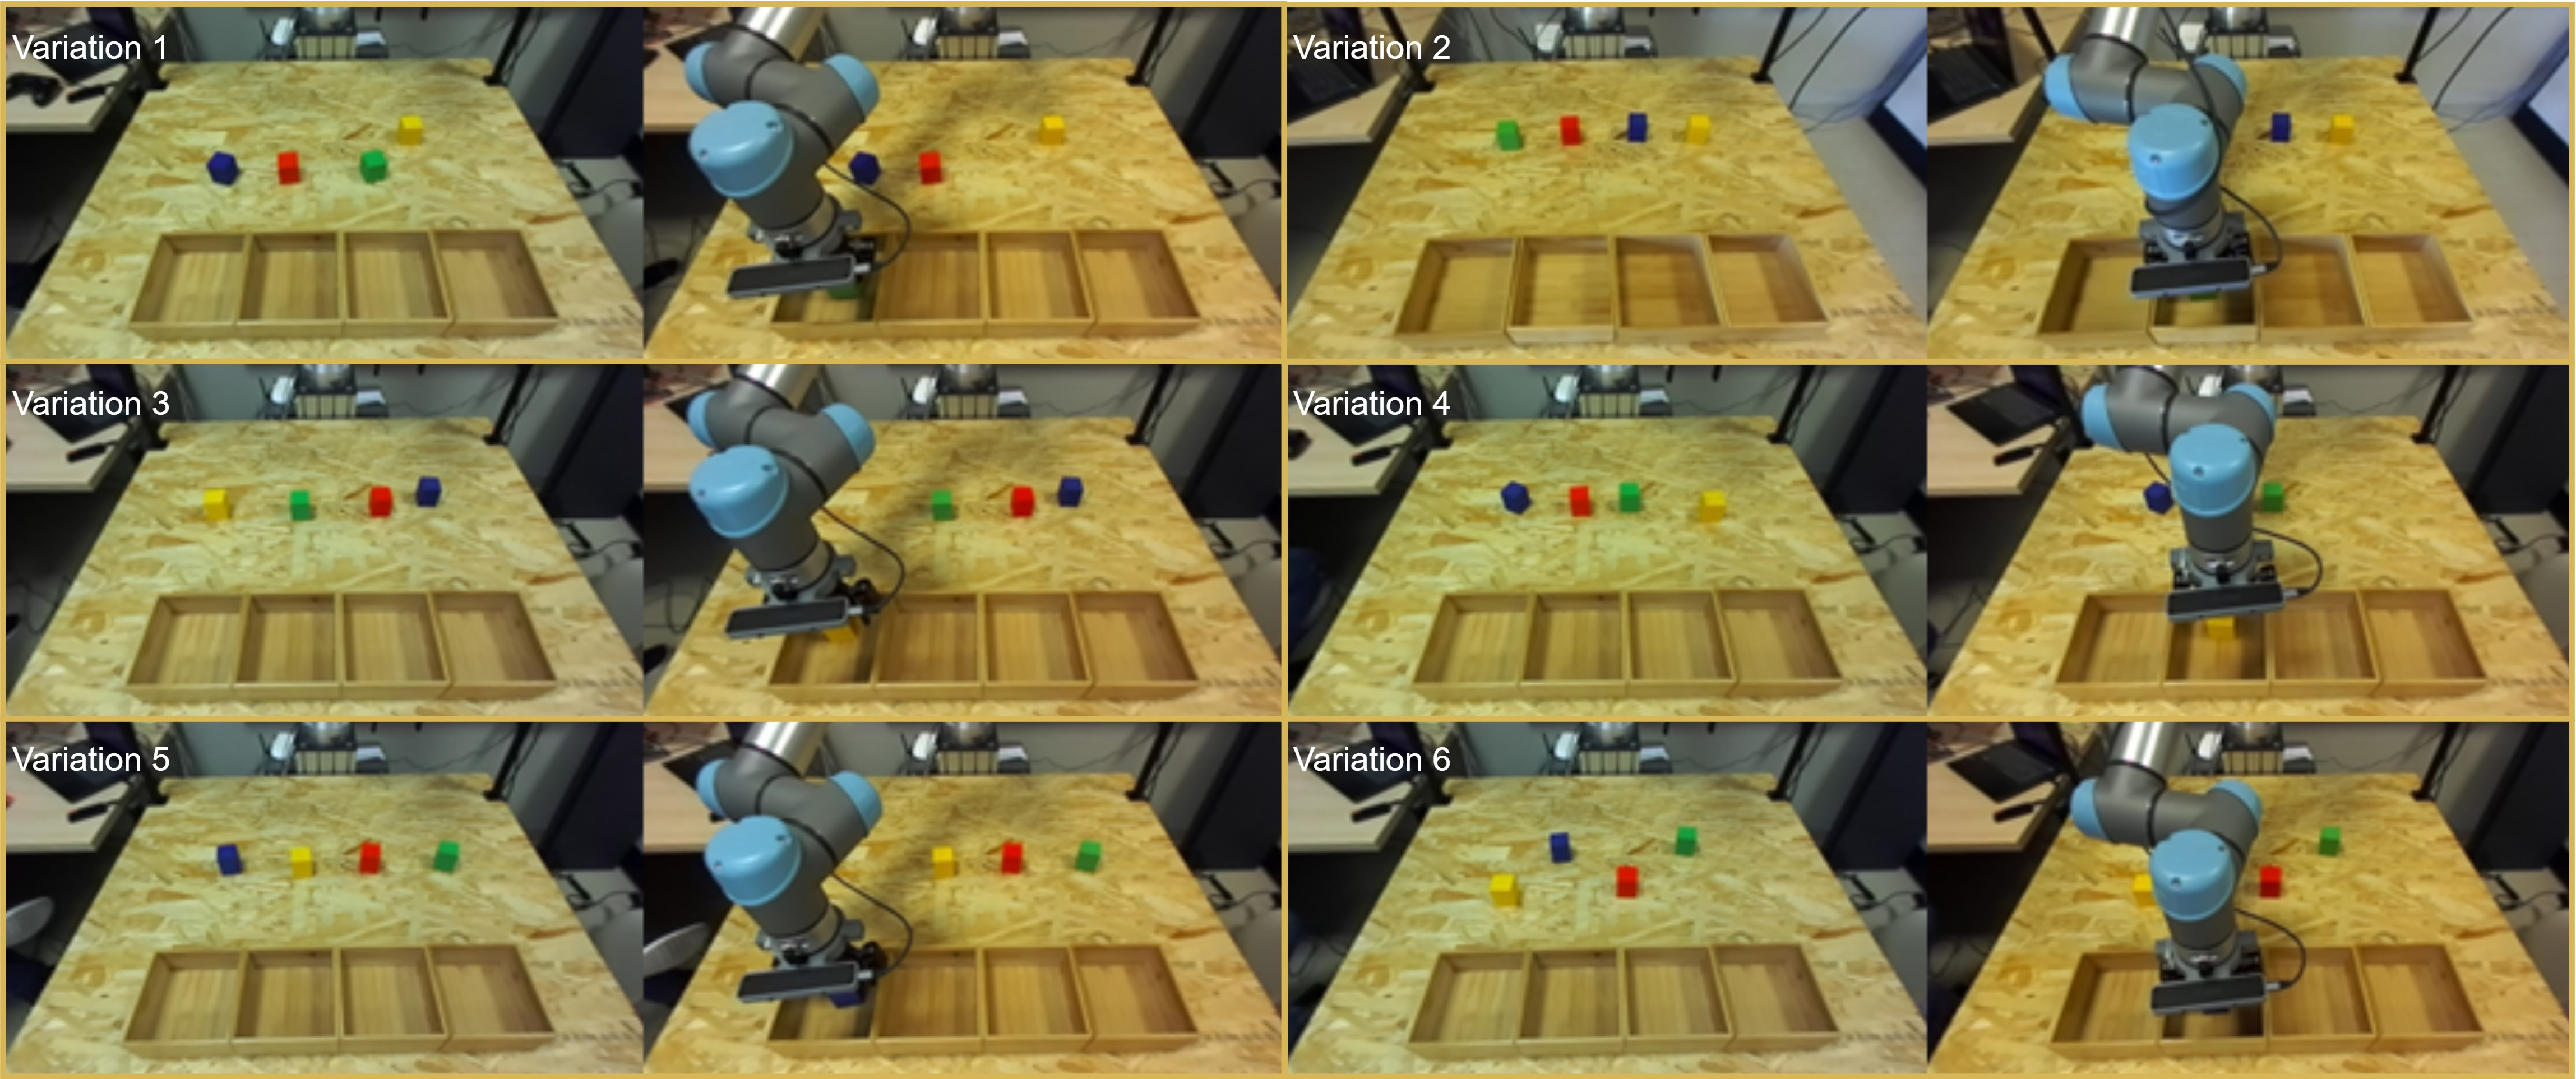
\includegraphics[width=1.0\textwidth]{figures/images/ch5/real_world_dataset.jpg}
    \caption{Set of variations used in the real-world robot evaluation. For each variation, the first and last frames are provided}
    \label{fig:real_world_dataset}
\end{figure}


Figure \ref{fig:real_world_dataset} represents the 6 variations used in the real-world validation. As can be noted, these are essentially the first six variations of the Pick-Place Task used in the simulation environment.

A preliminary dataset composed of \textbf{40 trajectories} for each variation has been collected by teleoperating the robot with a console controller. Regarding the object placement, the same algorithm described in Section \ref{sec:ocpl_dataset} was applied. This means that the set of 4 bins ($15 \times 15 \times 7$ cm) was fixed in position, while the 4 boxes ($4 \times 4 \times 6$ cm) could vary in their position within a region of $60$ cm in length and $15$ cm in height. 

In this extensive placement area, a specific protocol was implemented for collecting the trajectories. The protocol dictates how the objects are positioned within the picking region. The various placements of the target object are illustrated in Figure \ref{fig:box_placement}. Although the workspace may appear somewhat limited, this dataset is the first real-world dataset in the context of Visual-Conditioned Imitation Learning to encompass such a large operational space. In contrast, other works are either restricted to simulation environments \cite{dasari2021transformers_one_shot,mandi2022towards_more_generalizable_one_shot} or present very simple scenarios where objects are placed in a much smaller area \cite{mandlekar2022matters}.
\begin{figure}[t]
    \centering
    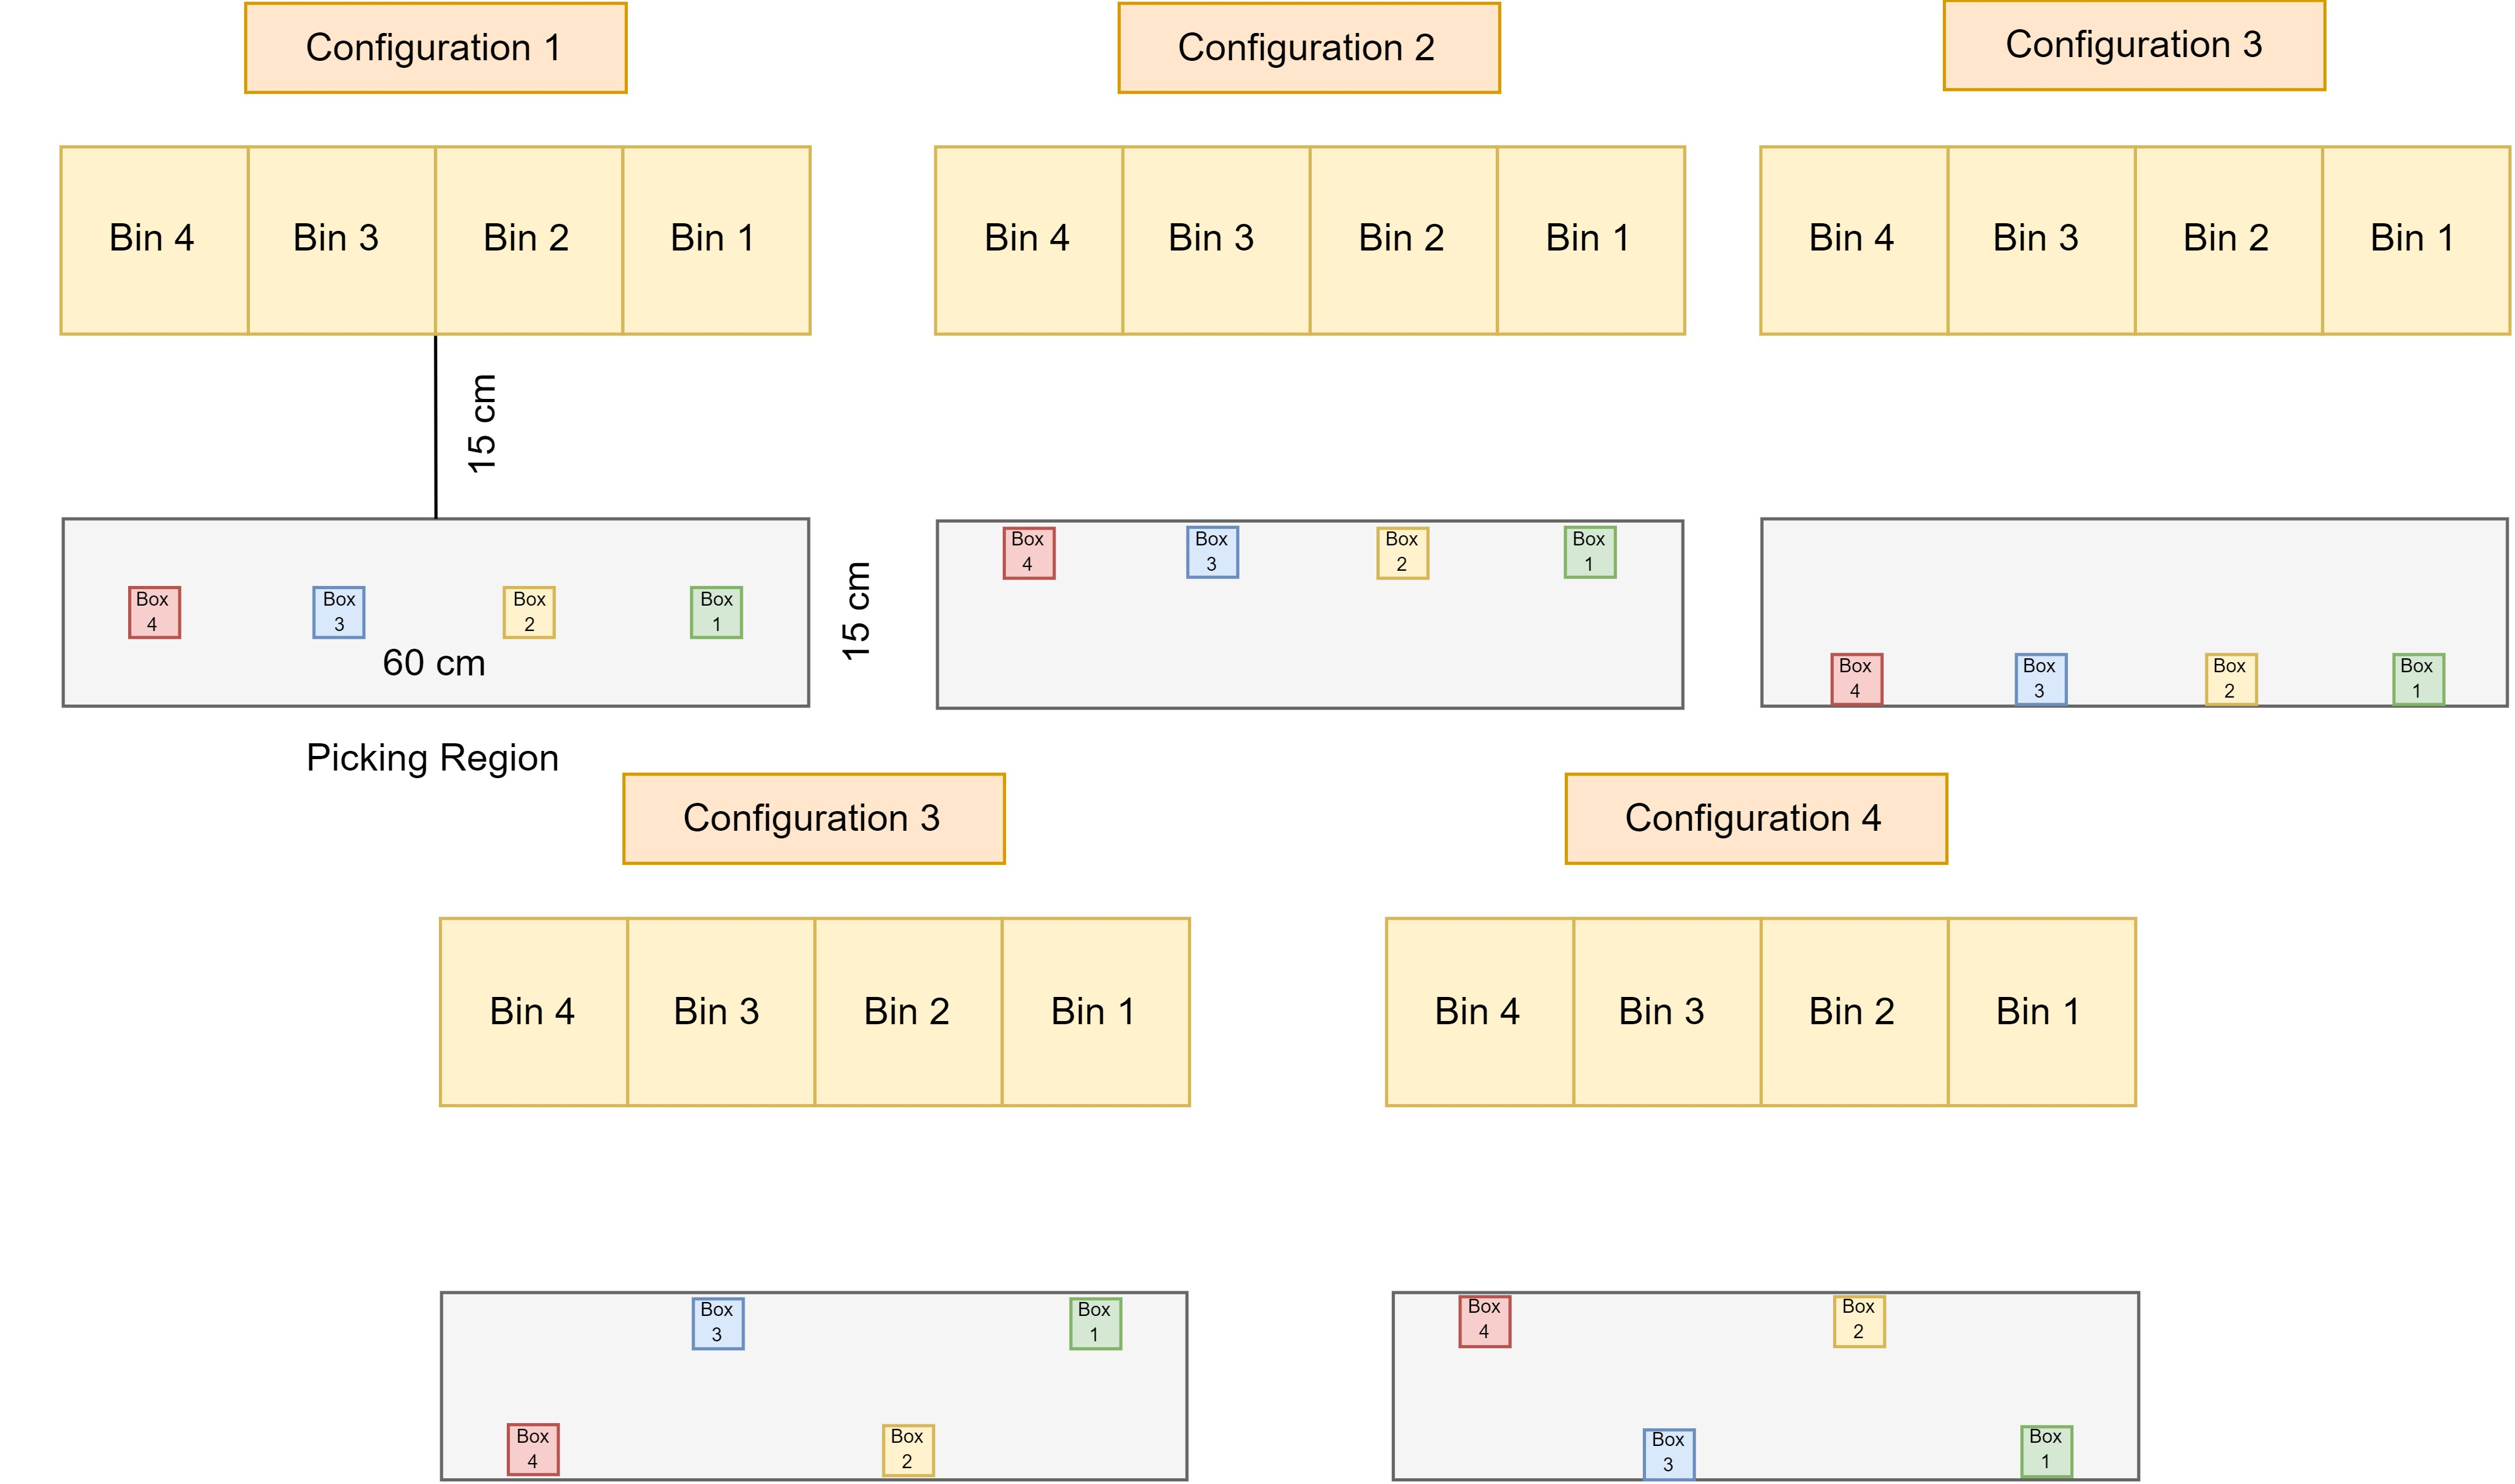
\includegraphics[width=0.8\textwidth]{figures/images/ch5/box_placement.jpg}
    \caption{Placement configuration used for the trajectory collection. For each placement configuration, 4 trajectories were collected. The target object initially starts at the rightmost position, and in each subsequent trajectory, the box is moved to the adjacent position. This process is then repeated twice, each time with a different object orientation, resulting in a total of 40 trajectories for a given configuration.}
    \label{fig:box_placement}
\end{figure}

% \smalltodo{add figure}
% \smalltodo{add figure}
Trajectories are collected through teleoperation the robot is controlled in its operational space, with the controller that sends continous velocity commands on a specific axis, this velocity command is defined by the value read by the controller's potentiometers.
During teleoperation different informatin are recorded:
\begin{itemize}
    \item \textit{Images} from the front, laterals and gripper cameras, both RGB and Depth images are recorded.
    \item \textit{Proprioceptive information} like joints positions and velocities.
    \item \textit{Trajectory state}, which is manually changed by the human operators based on the task state. The phases are:
        \begin{enumerate}
            \item \textit{Start}, this phase starts at the beginning of the trajectory till the robot gripper is perpendicular to the target object.
            \item \textit{Approaching}, this phase starts when the robot approaches the target object with its discending movement.
            \item \textit{Picking}, this phase is characterized by the gripper that is ready to be closed to pick the object, and contains the closing command.
            \item \textit{Moving}, this phase starts after the robot picks the object and lift it from the table, this phase ends when the gripper is perpendicular to the target bin.
            \item \textit{Placing}, this phase starts when the robot is ready to place the object, starting the discending phase towards the target bin, this phase also contains the opening command.
        \end{enumerate}
    \item \textit{Objects bounding boxes}, which are are generated automatically, requiring minimal input from human operators. At the start of the trajectory, the operator needs to specify the position of each object in the scene, including both boxes and bins. This is done by displaying the first frontal frame of the trajectory and clicking on the objects with the cursor. The positions, initially defined in discrete pixel-space, are then converted into continuous world-space through a series of transformations, using the camera's intrinsic and extrinsic parameters. The extrinsic parameters are obtained via a calibration procedure that uses ARUCO markers.
\end{itemize}
The overall space coverage of the real-world dataset is shown in Figure \ref{fig:real_world_coverage}. As can be observed, the coverage is more limited and considerably noisier compared to the simulated dataset, even when restricted to the same variations. This is due to the collection of fewer trajectories and the use of teleoperation without any hand-written control rules, which typically generate smoother and more deterministic robot behaviors. These limitations introduce additional challenges in learning a robust control policy, especially for generalizing to different placements of the target object. This issue will be addressed in this thesis by initially training the policy in the simulation environment, where a complete dataset is available, and then fine-tuning it on the noisy real-world dataset.
\begin{figure}[t]
    \centering
    
\includegraphics[width=1.0\textwidth]{figures/images/ch5/real_world_dataset_coverage.jpg}
    \caption{(Left) Trajectory distribution along the x-y axis of the real-world dataset. (Right) Trajectory distribution along the x-y axis of the simulated dataset, constrained to the same variations and number of trajectories as the real-world counterpart. It can be observed that the real-world dataset exhibits a much sparser and noisier distribution, due to the fact that the trajectories are collected via teleoperation.}
    \label{fig:real_world_coverage}
\end{figure}

% \smalltodo{add figure}
\section{Results}
\label{sec:real_results}


\section{Conclusion}
In conclusion, this chapter presented the experimental validation of the proposed methods in a real-world scenario. Both the proposed detectors and control policies were tested in a single-task multi-variation scenario.

Regarding the conditioned object detectors, it was observed that the system successfully identified the target object even when the video demonstration was provided by a simulated robot, which had a different visual appearance compared to the real robot. This highlights the strong potential of the proposed method to generalize across different demonstrators and environments, such as human demonstrators. Generally, the patterns observed in the simulated environment were replicated in the real-world tests, where the system consistently identified the target object during the reaching phase but generated false positives during the manipulation and placing phases. However, the drop in precision was more pronounced in the real-world setting due to occlusions and inaccuracies in the automated bounding box generation process.

As for the control policies, the results demonstrated that the proposed architectures were able to successfully complete tasks in real-world scenarios. The object conditioned control policies consistently reached the target object, leading to successful task completion. Across all variations of the proposed method, an average reaching rate of $85.40\%$ was achieved, compared to $14.12\%$ for the MOSAIC baseline. This indicates that object priors can be effectively leveraged to simplify the control problem, resulting in a policy that consistently reaches the target object, even when using a dataset with low-quality demonstrations. In terms of overall success rate, the MOSAIC-COD module achieved the highest rate of $55.00\%$. While this may not seem particularly high, it is a promising result given the challenging nature of the dataset, which contains fewer and noisier trajectories compared to the simulated environment. This result becomes even more significant when compared to the MOSAIC baseline's success rate of $0.00\%$.

Generally speaking, the most critical error observed involves collisions with the target object. This type of error could be significantly reduced by integrating additional exteroceptive modalities, such as depth images from the gripper camera. Incorporating this data would enable the system to better detect the target object and avoid collisions during the picking phase, which is expected to result in a substantial improvement in the overall success rate.
\chapter{Graph Neural Network for heuristic estimation}
\ref{ch:gnn_planning_systems}
% The goal of this chapter is to evaluate and review the possibility of leveraging Graph Neural Network (GNN) in the context of robotics learning. Specifically, this chapter will divided into different sections: Section \ref{sec:gnn_related_works} will discuss the related works and in general the application of GNN in the context of Learning from Demonstration.
This chapter presents an initial exploration of how learning algorithms could enhance the capabilities of the proposed system. The system, as introduced, operates based on a control policy capable of handling single-step tasks, meaning tasks that consist of a single manipulation step. However, in real-world applications, tasks are often more complex, involving multiple steps. For instance, a task may require performing several pick-and-place operations, with the additional constraint that they must follow a specified sequence. In traditional robotics, such problems are classified as \textit{Planning Problems}, where the objective is to produce a sequence of \textbf{high-level actions} that move the system from an initial state to a desired goal state. 

The primary idea for future work is to integrate planning algorithms into the current framework. This would enable the planning system to generate the high-level action sequence, while the proposed OCCP module executes the corresponding low-level actions, directing the robot to fulfill the tasks derived from the high-level commands.

The purpose of this chapter is twofold: first, to review state-of-the-art methods for solving planning problems, encompassing both classical planning approaches and modern data-driven techniques (Section \ref{sec:gnn_related_works}); and second, to present preliminary results that demonstrate the applicability of these methods within the specific context of the system under discussion, with a comparative analysis between these data-driven approaches and traditional planning algorithms (Section \ref{sec:gnn_experimental_results}).


\section{Related Works}
\label{sec:gnn_related_works}
This section reviews prior research on the application of Graph Neural Networks (GNNs) to robot learning tasks. As shown in Figure \ref{fig:gnn_taxonomy}, GNNs can be applied in various ways; however, they all share a common underlying principle: leveraging GNNs capability to explicitly model dynamic relationships between objects involved in robotic manipulation. This ability to capture and represent interactions between objects is vital for effective robotic perception, planning, and task execution, as these relationships often govern the complexity and success of manipulation tasks.


\begin{figure}[t]
    \centering
    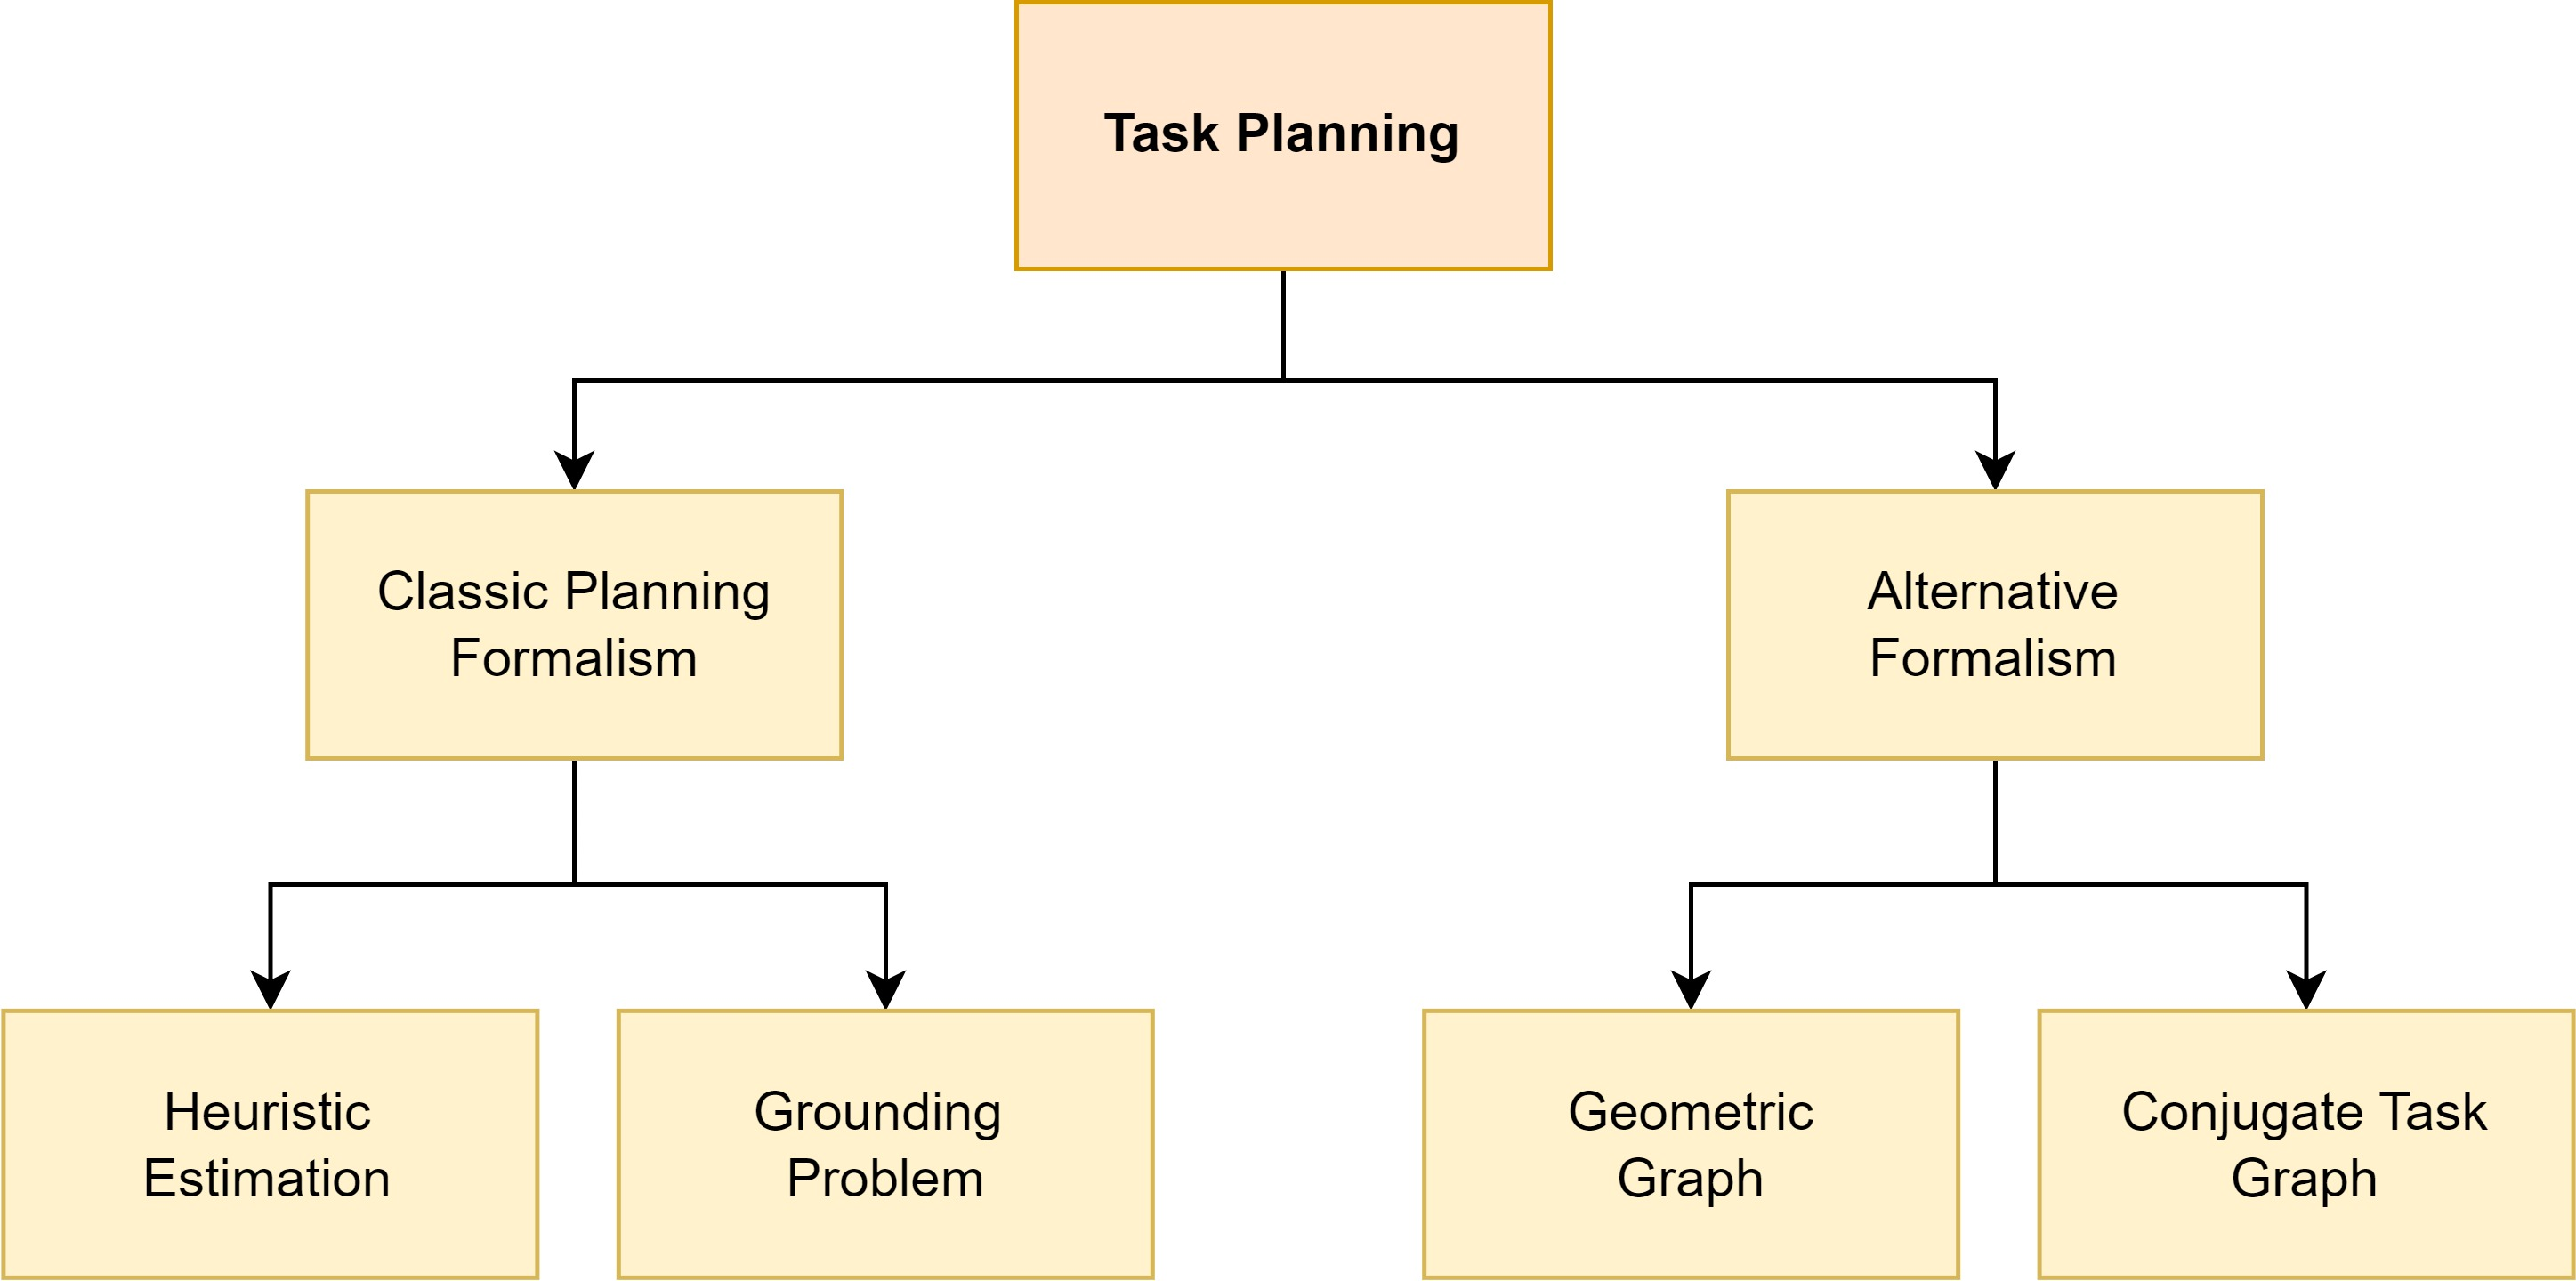
\includegraphics[width=0.8\textwidth]{figures/images/ch4/gnn_taxonomy.jpg}
    \caption{Proposed taxonomy for GNNs methods used in the context of robotic learning.}
    \label{fig:gnn_taxonomy}
\end{figure}


In general, most research has focused on solving \textit{task planning} problems. According to classical literature \cite{geffner2013concise}, a task-planning problem can be defined as a state-transition model $\Pi = \left( S, A, s_{0}, G \right)$, where $S$ is the set of states, $A$ is the set of actions, $s_{0}$ is the initial state, and $G$ is the goal state. Here, an action $a \in A$ is a function that maps a state $s \in S$ to a new state (successor) $a(s)$, i.e., $a: S \rightarrow S$. Essentially, a plan is a sequence of actions $\tau = a_{1}, a_{2}, \dots, a_{n}$ that enables the system to transition from the initial state $s_{0}$ to the goal state $s_{n} = a(s_{n-1}) = G$. Various approaches have been proposed to solve the problem of finding a plan given a specific initial and goal state. These approaches either adhere to the classical PDDL formalism \cite{aeronautiques1998pddl}, and thus fit within the traditional planning framework, or introduce novel representations that do not rely on PDDL to address the planning problem.

This review begins by examining methods that follow the \textit{Classic Planning Formalism}  (Section \ref{sec:pddl_formalism}), followed by a brief discussion of novel approaches that do not use this kind of formalism (Section \ref{sec:gnn_alternative_formalism}).

\subsection{Classic Planning Formalism}
\label{sec:pddl_formalism}
In this section, we will describe the methods that follow the classic task-planning formalism. Before introducing the methods, it is crucial to define the formalism with a set of foundational definitions.

Task-planning is a well-known problem that has been studied for many years. One of the most influent formalizations, still widely used today, is STRIPS (Stanford Research Institute Problem Solver) \cite{fikes1971strips}, which was developed in the 70s. STRIPS was initially an automated planning solver, but its primary contribution lies in its definition of a planning problem, which has served as the foundation for much of the research in subsequent decades.

According to the STRIPS formalism, a planning task is defined as a tuple $\Pi = (P, A, s_0, G, c)$, where:
\begin{itemize}
    \item $P$ is a set of propositions (also called facts).
    \item $A$ is a set of actions.
    \item A state $s$ is a subset of predicates, $s \subseteq P$, where $s_0$ is the initial state,
    \item $G \subseteq s$ represents the goal conditions.
    \item $c: A \leftarrow R$ is the cost function, which assign to an anction $a \in A$ a real-value, $c(a)$ representing the cost of performing a given action.
\end{itemize}

An action $a \in A$ is defined as a tuple $a = \left(pre(a), add(a), del(a)\right)$, where $pre(a), add(a), del(a) \subseteq P$. These represent:
\begin{itemize}
    \item $pre(a)$: the preconditions (i.e., predicates that must be true to perform the action).
    \item $add(a)$: the added conditions (i.e., predicates that become true after the action is executed).
    \item $del(a)$: the deleted conditions (i.e., predicates that become false after the action is executed).
\end{itemize}
with the constraint that $add(a) \cap del(a) = \emptyset$. According to this formalism, an action is applicable in a state $s$ if $pre(a) \subseteq s$, and it results in the successor state $s' = (s \setminus del(a)) \cup add(a)$.

Building on these foundational concepts, the \textbf{Planning Domain Definition Language} (PDDL) was introduced in the 90s \cite{aeronautiques1998pddl}. PDDL is a human-readable format for describing automated planning problems. It provides a way to describe, the possible states of the world, the set of available actions, where each action description includes the prerequisites and the effects of the action, a specific initial state of the world and a specific set of desired goals. 

PDDL separates the model of a planning problem into two main components:
\begin{enumerate}
    \item The domain description, which defines the elements that are common across all problems within a given domain.
    \item The problem description, which specifies the specific planning problem, including the initial state and the goals to be achieved.
\end{enumerate}

\input{figures/ch4/example_domain_problem.tex}

Figure \ref{fig:domain_problem} provides examples of domain and problem definitions for the Blocks-World environment. As shown, when using the PDDL formalism, it is essential to fully define the elements of the world (e.g., blocks), the available actions (e.g., pick-up), along with their corresponding preconditions (i.e., predicates that must be true for the action to be executed) and postconditions (i.e., the effects of the actions). In the problem definition, specific instances of objects in the environment are specified, along with the initial state and goal state, both of which are defined based on the predicates available in the domain definition.

Once the problem is defined using the PDDL formalism, a complete parameterized instance must be specified to obtain a solution to the planning problem. This involves solving what is known as the \textbf{grounding problem}. During this process, all predicate and action variables must be instantiated with the objects defined in the problem. For instance, in the example shown in Figure \ref{fig:domain_problem}, the variable \( x \) is replaced with objects \( b1 \), \( b2 \), and \( b3 \) from the problem definition, leading to a complete enumeration of all predicates and actions. The result of this process is known as the \textit{Grounded Planning Problem}, which follows the same formalism as the STRIPS representation described earlier.

The grounded problem then serves as the input for planning algorithms, such as the well-known Fast Downward \cite{helmert2006fast} or LAMA \cite{richter2010lama}. While delving into the specifics of these algorithms is beyond the scope of this section, it is crucial to note that they are essentially \textit{search algorithms}. Given a state-space represented as a graph, which is derived from the Grounded STRIPS representation, these algorithms compute the (estimated) the shortest path in the state-space, connecting the source node (representing the initial state) to the target node (representing the goal state).

The limitations of these approaches have been well-known for a long time. Specifically, these algorithms do not scale well as the size of the problem (in terms of actions, predicates, and objects) increases. There are two main areas where higher problem dimensionality can cause performance issues:

\begin{enumerate}
    \item \textit{Search Phase}, as the dimensionality of the problem increases, the state-space expands correspondingly. This increases the time required to explore the state-space and find a solution path.
    \item \textit{Grounding Problem}, as the problem dimensionality grows, the time needed to generate a complete enumeration of all object combinations grows exponentially.
\end{enumerate}

To address the first issue, research has focused on developing methods to accelerate the search phase by introducing \textit{heuristics} that guide the search more efficiently towards the goal state. For the second issue, the literature has proposed methods that perform \textit{partial} grounding, concentrating on the action instances that are most relevant to the specific problem instance. Examples of these methods will be discussed in the following two paragraphs.

Here, a heuristic is a function $h: S \rightarrow \mathbb{R}$, which maps a state $s \in S$ to a real value $h(s)$, representing an estimate of the cost to reach the goal state from the state $s$. The optimal heuristic, denoted $h^{*}(s)$, is the heuristic that gives the exact cost of the optimal plan to reach a goal state from $s$. A heuristic is considered \textit{admissible} if it never overestimates the actual cost, i.e., $h(s) \leq h^{*}(s), \forall s \in S$. By utilizing the heuristic cost, a search algorithm can focus on exploring the most promising states instead of performing an exhaustive search of the entire state space.

In the context of task planning, a common heuristic is computed by solving the \textbf{Relaxed-STRIPS} problem. This is a simplified version of the STRIPS problem, where the delete conditions ($del$) are ignored, i.e., an action $a$ is represented as $a = \left(pre(a), add(a), \emptyset \right)$. The Relaxed-STRIPS problem is easier to solve because removing the $del$ conditions relaxes some of the constraints, allowing the state to include predicates that logically cannot be true simultaneously. By solving this relaxed problem, an estimated cost for reaching the goal from a given state can be computed. This approach has been used in well-known algorithms such as Fast-Downward \cite{helmert2006fast} and combined with novel heuristics in LAMA \cite{richter2010lama}.

\paragraph*{Heuristic Estimation}\mbox{}\\
In this paragraph the methods that methods that propose GNN for computing heuristics estimation through the usage of GNNs are discussed. Specifically, the review will focus on two recent works \cite{shen2020learning,chen2024learning}.

The first remarkable work towards the use of GNN for heuristic estimation was proposed by authors of \cite{shen2020learning}. Here, authors started from the idea to leverage data-driven approaches to learn an heuristic function, and explore the possibility of such methods to generalize to different cardinalities and problems, and comparing the performance of such methods with classic heuristic functions.

The first step to solve this problem is related to the definition of the input. Specifically, the authors started by the Relaxed-STRIPS formulation. The STRIPS problem can be easly formulated as a graph if the following observations are done:
\begin{itemize}
    \item A node, can be described a predicate which can be either a pre-condition or an added condition.
    \item The edge is represented by the action that connects the pre-conditions to the added-conditions. 
\end{itemize}
\smalltodo{add figure}
Figure \ref{} illustrates the mapping of predicates and actions to graph nodes and edges. As can be observed, an action connects multiple nodes. To model this, the authors use a generalized graph structure known as a \textit{hypergraph}. Formally, a hypergraph is defined as a triple $G = (u, V, E)$, where $V = \left\{ \textbf{v}_{i}: i \in \left\{1, 2, \dots, N^{v} \right\} \right\}$ is the set of $N^{v}$ vertices, and $E = \left\{ (e_{k}, R_{k}, S_{k}): k \in \left\{1, 2, \dots, N^{e} \right\} \right\}$ is the set of $N^{e}$ hyper-edges. In this structure, $R_{k}$ is the receiver set, containing the indices of the nodes for which the $k$-th edge acts as an incoming edge, and $S_{k}$ is the sender set, containing the indices of the nodes for which the $k$-th edge acts as an outgoing edge. Then, $\textbf{v}_{i}$ is the node embedding, which has been implemented as a binary-vector $v_i = [x_s, x_g]$, where $x_s, x_g \in \left\{0,1\right\}$. $x_s=1$ iff the i-th predicate is true in the state s and $x_g=1$ iff the predicate is true in the goal-state. While, $e_{k}$ is the edge embedding, $e_k = [c(a_k), |Pre(a_k)|, |Add(a_k)|]$, where $c(a_k)$ is the cost of the operator, $|Pre(a_k)|$ is the number of pre-condition and $|Add(a_k)|$ is the number of added condition.

Once the graph structure has been defined, the module that processes this input can be described. Specifically, the authors propose leveraging the concept behind the \textit{Interaction Network} \cite{battaglia2016interaction}. The architecture, depicted in Figure \ref{}, implements the computational flow shown in Figure \ref{}, and can be divided into the following three steps.

\begin{enumerate}
    \item The \textit{Encoding Block} consists of two functions, $\phi^{e}$ and $\phi^{v}$, both implemented as Multi-Layer Perceptrons (MLPs). These functions transform the initial binary inputs into higher-dimensional representations, specifically, $\phi^{e}(e_j)$ produces $e_{hid}^{0}$ and $\phi^{v}(v_i)$ produces $v_{hid}^{0}$, where both $e_{hid}^{0}$ and $v_{hid}^{0} \in \mathbb{R}^{32}$. This step expands the original binary vectors (of size 2 or 3) into 32-dimensional vectors.

    \item The \textit{Core Block} implements the Message-Passing Iterative Procedure and is divided into the following steps:

        \begin{enumerate}
            \item \textit{Edge Block}: For each edge (representing an action), $e_{hid,j}^{t-1}$ is generated by concatenating the embeddings of the receiver and sender nodes associated with the edge. An MLP encoder is then applied to this concatenated information to create a new edge representation $e_{hid,j}^{t}$.

            \item \textit{Node Block}: Similar to the Interaction Network, only the receiver nodes' states are updated. The edge information influencing each receiver is aggregated by summing the embeddings of the incoming edges using the function $\rho^{e \rightarrow v}$. The node input is constructed by concatenating the incoming edge embeddings $e_{hid,j}^{t}$, the initial node embedding $v_{hid,i}^{0}$, and the previous node state $v_{hid,i}^{t-1}$. This concatenated input is then passed through an MLP to generate the updated node representation $v_{hid,i}^{t}$.

            \item \textit{Global Block}: This block updates the global graph representation by aggregating both node and edge embeddings using the functions $\rho^{e \rightarrow u}$ and $\rho^{v \rightarrow u}$, respectively. The aggregated information is passed through an MLP to produce the new global graph representation.
        \end{enumerate}

    \item The \textit{Decoding Block} acts as a decoder, implemented as an MLP. It takes the updated global graph representation as input and generates a heuristic value for a given state, aiding in the decision-making process.
\end{enumerate}

The operations in the core block are repeated for $M$ iterations, where $M = 10$ in this work.
The system is trained by minimizing the loss function defined in Equation \ref{equation:loss_func}. Here, $h^{*}(s)$ represents the ground truth heuristic value for state $s$, obtained by solving the training planning problem with a classical planning algorithm.
\begin{equation}
    \mathcal{L}_\theta(\mathcal{B})=\frac{1}{|\mathcal{B}|} \sum_{\left(G, h^*(s)\right) \in \mathcal{B}} \frac{1}{M} \sum_{t \in \{1, \ldots, M\}}\left(h_t^\theta(G)-h^*(s)\right)^2
    \label{equation:loss_func}
\end{equation}

Interesting results were obtained during the experiments. Notably, the system demonstrated the ability to learn both domain-dependent heuristics (when tested on the same domain it was trained on) and domain-independent heuristics (when tested on a different domain). This shows that the trained GNN was capable of generating meaningful heuristic values that could be effectively used by search algorithms like A*. However, a general drawback of this approach is the time required to compute the heuristic, particularly when the model is run on a CPU instead of a GPU, which significantly impacts performance.

Development of such work was proposed by \cite{chen2024learning},
\smalltodo{ToContinue}

\paragraph*{Grounding Problem}\mbox{}\\
As stated before, one of the preliminary problem to solve, before running the search algorithm, is the Grounding Problem. In this problem 
\smalltodo{ToContinue}
\subsection{Alternative Formalism}
\label{sec:gnn_alternative_formalism}

This section discusses methods that do not rely on classical planning but instead use a graph-based environment representation, where nodes represent objects and edges denote relationships or possible actions. This structure allows Graph Neural Networks to process the graph and select the next high-level action for the robot. The following paragraphs explore different environment representations and how the network's output is translated into robot actions.

\paragraph*{Geometric Graph} \mbox{}\\
This section explores methods based on the concept of the Geometric Graph. In its initial formulation \cite{lin2022efficient}, a Geometric Graph is a scene representation where nodes correspond to task-relevant entities, such as objects and their target positions. A fully connected graph is constructed by linking two types of nodes: \textit{object} nodes, which represent current instances of objects with their positions as attributes, and \textit{goal} nodes, which represent the desired final positions of these objects, also characterized by spatial attributes.

Using this representation, a GNN can be trained to perform node classification. At each step, an object node and a goal node are selected, representing the object to move and its target position. With these selections, a pick-and-place primitive can be executed. An example of this inference process is shown in Figure \ref{fig:geometric_graph_computation}.
\input{figures/ch4/geometric_graph_computation.tex}
% \smalltodo{add figure}

A similar approach is presented in \cite{di2023one}, where two GNNs are trained separately to classify an object node and a goal node.

While these methods are noteworthy because they can solve multi-step tasks through supervised learning without relying on a planning algorithm, they have significant limitations. The most notable is their dependency on knowing both the current and target positions of the objects. In these early studies, such information is provided either by the simulation environment or by using special markers on objects in real-world settings to facilitate position estimation.

To address these limitations, the authors in \cite{zhu2021hierarchical} extended the Geometric Graph concept and proposed a new representation called the \textit{Symbolic Scene Graph}. In this framework, a 3D Object Pose Estimation module is used to extract objects from the scene, constructing a geometric graph. Edges are then added based on predefined relationships (e.g., ``can1 on shelf A", as illustrated in Figure \ref{fig:geometric_scene_graph}). The next step in the planning process is determined using a Neuro-Symbolic Task Planning module \cite{xu2019regression}, which takes the current Symbolic Scene Graph and the goal (expressed as desired predicates, i.e., relationships between objects) as input. This module outputs the next action, expressed as a subgoal achievable with a single motion primitive.
\input{figures/ch4/geometric_scene_graph.tex}

While this method showed promising results, including reduced computation times compared to the PDDLStream \cite{garrett2020pddlstream} baseline, it has limitations. The primary challenge lies in the cognitive module, which relies on 3D object pose estimation. This technique is only robust and reliable when used with pre-known objects.

\paragraph*{Conjugate Task Graph} \mbox{}\\
The Conjugate Task Graph (CTG) \cite{huang2019neural} addresses challenges in constructing traditional Task Graphs, where nodes represent states and edges represent transitions. For novel tasks, mapping states to new nodes is often infeasible. In contrast, the CTG uses nodes to represent actions, with edges implicitly representing states and their preconditions (Figure \ref{fig:conjugate_task_graph}).
\input{figures/ch4/conjugate_task_graph.tex}
Based on this representation, and assuming all possible actions have been observed in the training set, it is possible to build and train a modular architecture composed of the following components:
\begin{itemize}
    \item \textit{Demo Interpreter}: A Convolutional Neural Network \\ trained to extract the sequence of actions performed by a robot from a given demonstration. This sequence of actions is used to construct an initial graph.
    
    \item \textit{Graph Completion}: A Graph Neural Network trained to complete the graph produced by the Demo Interpreter. This module predicts the missing edges in the graph, representing unseen transitions between actions.
    
    \item \textit{Node Localization}: A Multi-Layer Perceptron that, given the current observation's encoding and the embeddings of the nodes in the graph, predicts the node corresponding to the action the robot is currently performing.
    
    \item \textit{Edge Localization}: Another MLP that, given the current observation's encoding and the node embeddings, predicts the edge representing the next transition and, consequently, the next action the robot should take.
\end{itemize}

The complete architecture was trained end-to-end, and experimental results demonstrate its effectiveness in multi-step tasks, such as object ordering and stacking. The CTG representation enables the policy to generalize to novel sequences of actions, making it particularly well-suited for tasks like object ordering.

However, this approach fails to generate valid paths when the demonstration includes out-of-distribution observations, produced by sequences of actions that were never encountered in the training set. Additionally, experimental results reveal that this method struggles to perform tasks requiring more than 6 steps. This limitation arises mainly from the Demo Interpreter module, which must generate long action sequences to instantiate the CTG.


In conclusion, with respect to the discussed method, the goal of this chapter is to evaluate and assess the feasibility of using data-driven methods for heuristic estimation within a specific domain of interest. This evaluation aims to explore the potential of leveraging such methods in \textbf{future works}, where integrating low-level policies within high-level planning tasks could enable generalization to multi-step tasks.

\section{Experimental Results}
\label{sec:gnn_experimental_results}
In this section, the experimental results are presented. These results are preliminary within the context of this thesis and primarily aim to evaluate the performance and limitations of using GNNs for learning heuristics, specifically through the assessment of the STRIPS-HGN method proposed in \cite{shen2020learning}.

The method was tested in the well-known \textit{BlockWorld} domain \cite{slaney2001blocks}. This domain consists of a single object type, the \textbf{block}. 
This domain then, contains five predicates, and four actions that are listed below: 

\begin{itemize}
    \item \textit{On}: True if block $x$ is on block $y$.
    \item \textit{On-Table}: True if block $x$ is on the table.
    \item \textit{Clear}: True if block $x$ has no object on top, making it available for manipulation.
    \item \textit{Handempty}: True if the robotic gripper is not holding any object.
    \item \textit{Holding}: True if the robotic gripper is holding block $x$.

    \item \textit{Pick-Up}: Picks up block $x$ if it is clear, on the table, and the gripper is empty.
    \item \textit{Put-Down}: Places the block currently held by the gripper onto the table.
    \item \textit{Stack}: Stacks block $x$ (held by the gripper) onto a clear block $y$.
    \item \textit{Unstack}: Removes block $x$ from on top of block $y$ (if block $x$ is clear) and picks it up with the gripper.
\end{itemize}

For the experiments, 50 problem instances of varying complexity were generated, with complexity measured by the number of blocks, ranging from 3 to 15. The STRIPS-HGN was trained on a subset of problems with block counts between 5 and 10. Testing was conducted in two scenarios:

\begin{itemize}
    \item \textit{In-Training Distribution}: The model was tested on new problems with complexities within the same range as the training data.
    \item \textit{Out-of-Training Distribution}: The model was tested on problems with unseen complexities (3, 4, 11, 12, 13, and 15 blocks).
\end{itemize}

The ground-truth heuristic ($h^{*}$) was computed by solving each problem instance using the Scorpion planning solver \cite{seipp2020saturated}, in a configuration that ensure the optimality of the solution. In this case, the heuristic is represented as the number of actions needed to reach the goal state from the initial state.
% configured with the LAMA search algorithm \cite{richter2010lama}. While this setup does not guarantee path optimality, it provides the most reliable method for obtaining a solution across all 50 problem instances, regardless of task complexity, within a 16-minute time limit per instance.

The STRIPS-HGN performance was compared against several classic heuristics, including:
$h_{max}$, an admissible heuristic; $h_{add}$, a generally faster heuristic; $LM-cut$ \cite{richter2010lama}, a heuristic offering a balance between path optimality and speed. The STRIPS-HGN was also compared against itself with different numbers of planning steps (1, 5, and 10).

Moreover, different metrics have been proposed to compare the different algorithms. Specifically, the algorithms are compared with respect to:
\begin{itemize}
    \item \textit{Number of expanded nodes}, this measures the number of nodes that are traversed during the exploration of the state-space in order to find a given solution. This number is accumulated over the different problems of a given complexity, then the average and standard deviation is computed.
    \item \textit{Search time}, this measures the time needed for the algorithm to return a valid solution.  This number is accumulated over the different problems of a given complexity, then the average and standard deviation is computed.
    \item \textit{Plan length}, this measures the number of actions that are needed to reach a solution. This number is accumulated over the different problems of a given complexity, then the average and standard deviation is computed.
    \item \textit{Ratio of solution found}, this measures the ratio of number of times the search algorithm with a given heuristic returns a solution before a timeout of 5 minutes over all the number of problems.
\end{itemize}

\paragraph*{In-Training Distribution Generalization}\mbox{}\\
The first generalization test performed was related to the In-Training Distribution Generalization. This means that the algorithms are tested on 10 novel problem instances for each problem complexity.
The first results are related to the number of solution found, reported in Table \ref{table:in_distribution_cnt_success}. It can be noted how most of the heuristics are able to completely return a solution in the given timeout. This does not happen for the admissible heuristic $h_{max}$, which starts to not return a valid solution, starting from the complexity of 9 boxes. 

\begin{table}[t]
    \centering
    % \refstepcounter{table}
    \caption{Comparison of ``ratio of solution found'' on BlocksWorld domain across different complexities (Comp.). The table presents the results for $h_{max}$, $h_{add}$, $LM-cut$, and Strips-HGN with 1, 5, and 10 steps.}
    \label{table:in_distribution_cnt_success}
    \resizebox{\linewidth}{!}{%
    \begin{tabular}{|c|c|c|c|c|c|c|} 
    \hline
    \textbf{Comp.} & $\mathbf{h_{max}}$ & $\mathbf{h_{add}}$ & $\mathbf{LM-cut}$ & $\mathbf{Strips-HGN_1}$ & $\mathbf{Strips-HGN_5}$ & $\mathbf{Strips-HGN_{10}}$ \\ 
    \hhline{|=======|}
    5 & 1.00 & 1.00 & 1.00 & 1.00 & 1.00 & 1.00 \\ 
    \hline
    6 & 1.00 & 1.00 & 1.00 & 1.00 & 1.00 & 1.00 \\ 
    \hline
    7 & 1.00 & 1.00 & 1.00 & 1.00 & 1.00 & 1.00 \\ 
    \hline
    8 & 1.00 & 1.00 & 1.00 & 1.00 & 1.00 & 1.00 \\ 
    \hline
    9 & 0.00 & 1.00 & 1.00 & 1.00 & 1.00 & 1.00 \\ 
    \hline
    10 & 0.10 & 1.00 & 0.9 & 1.00 & 1.00 & 1.00 \\
    \hline
    \end{tabular}
    }
    \end{table}

To provide more insight into the generalization capabilities of STRIPS-HGN with respect to the training distribution, Tables \ref{table:in_distribution_avg_nodes_expanded}, \ref{table:in_distribution_avg_search_time}, and \ref{table:in_distribution_avg_plan_length} report key metrics, including the number of expanded nodes, search time, and plan length, respectively.

\begin{landscape}
\begin{table}
    \centering
    \caption{Mean and standard deviation of ``number of expanded nodes'' on the BlocksWorld domain across different complexities (Comp.). The table presents the results for $h_{max}$, $h_{add}$, $LM-cut$, and Strips-HGN with 1, 5, and 10 steps.}
    \label{table:in_distribution_avg_nodes_expanded}
    \resizebox{\linewidth}{!}{%
    \begin{tabular}{|c|c|c|c|c|c|c|} 
    \hline
    \textbf{Comp.} & $\mathbf{h_{max}}$ & $\mathbf{h_{add}}$ & \begin{tabular}[c]{@{}c@{}}\textbf{LM-}\textbf{cut}\end{tabular} & \begin{tabular}[c]{@{}c@{}}\textbf{Strips-}\textbf{HGN\textsubscript{1}}\end{tabular} & \begin{tabular}[c]{@{}c@{}}\textbf{Strips-}\textbf{HGN\textsubscript{5}}\end{tabular} & \begin{tabular}[c]{@{}c@{}}\textbf{Strips-}\textbf{HGN\textsubscript{10}}\end{tabular} \\
    \hhline{|=======|}
    5 & $98.80 \pm 97.06$ & $22.00 \pm 14.68$ & $24.40 \pm 23.30$ & $16.50 \pm 10.31$ & $\mathbf{12.40 \pm 3.29}$ & $12.90 \pm 3.70$ \\ 
    \hline
    6 & $643.70 \pm 430.89$ & $38.70 \pm 22.12$ & $35.10 \pm 22.56$ & $17.50 \pm 5.16$ & $\mathbf{17.10 \pm 6.77}$ & $17.30 \pm 6.42$ \\ 
    \hline
    7 & $3918.80 \pm 3124.33$ & $54.40 \pm 23.86$ & $83.70 \pm 100.14$ & $29.80 \pm 15.96$ & $27.90 \pm 12.29$ & $\mathbf{27.90 \pm 12.19}$ \\ 
    \hline
    8 & $77988.50 \pm 53611.24$ & $142.70 \pm 64.76$ & $481.60 \pm 558.93$ & $\mathbf{109.90 \pm 98.16}$ & $126.40 \pm 100.73$ & $119.90 \pm 94.02$ \\ 
    \hline
    9 & $154351.20 \pm 3673.33$ & $307.70 \pm 176.77$ & $758.90 \pm 1073.05$ & $99.70 \pm 94.47$ & $\mathbf{44.00 \pm 20.83}$ & $47.30 \pm 24.00$ \\ 
    \hline
    10 & $103801.70 \pm 11155.55$ & $366.20 \pm 320.12$ & $2799.70 \pm 4595.73$ & $235.90 \pm 270.38$ & $150.80 \pm 229.64$ & $\mathbf{95.70 \pm 110.71}$ \\
    \hline
    \end{tabular}
    }
    \end{table}
\end{landscape}
\begin{table}[t]
    \centering
    \caption{Mean and standard deviation of ``search time''  on the BlocksWorld domain across different complexities. The table presents the results for $h_{max}$, $h_{add}$, $LM-cut$, and Strips-HGN with 1, 5, and 10 steps.}
    \label{table:in_distribution_avg_search_time}
    \resizebox{\linewidth}{!}{%
    \begin{tabular}{|c|c|c|c|c|c|c|} 
    \hline
    \textbf{Complexity} & $\mathbf{h_{max}}$ & $\mathbf{h_{add}}$ & $\mathbf{LM-cut}$ & $\mathbf{Strips-HGN_1}$ & $\mathbf{Strips-HGN_5}$ & $\mathbf{Strips-HGN_{10}}$ \\ 
    \hhline{|=======|}
    5 & $0.05 \pm 0.05$ & $\mathbf{0.01 \pm 0.01}$ & $0.05 \pm 0.06$ & $0.13 \pm 0.08$ & $0.31 \pm 0.10$ & $0.57 \pm 0.20$ \\ 
    \hline
    6 & $0.53 \pm 0.31$ & $\mathbf{0.04 \pm 0.02}$ & $0.18 \pm 0.13$ & $0.20 \pm 0.07$ & $0.56 \pm 0.24$ & $1.05 \pm 0.41$ \\ 
    \hline
    7 & $4.10 \pm 2.99$ & $\mathbf{0.08 \pm 0.03}$ & $0.58 \pm 0.62$ & $0.36 \pm 0.18$ & $1.04 \pm 0.55$ & $1.74 \pm 0.97$ \\ 
    \hline
    8 & $95.44 \pm 53.45$ & $\mathbf{0.34 \pm 0.19}$ & $5.94 \pm 6.98$ & $1.68 \pm 1.55$ & $5.52 \pm 4.60$ & $9.73 \pm 8.03$ \\ 
    \hline
    9 & $300.00 \pm 0.00$ & $\mathbf{0.88 \pm 0.47}$ & $13.10 \pm 18.61$ & $1.79 \pm 1.44$ & $2.10 \pm 1.06$ & $4.11 \pm 2.28$ \\ 
    \hline
    10 & $289.29 \pm 32.15$ & $\mathbf{1.44 \pm 1.14}$ & $69.89 \pm 114.03$ & $4.79 \pm 5.35$ & $8.90 \pm 13.89$ & $11.05 \pm 14.90$ \\
    \hline
    \end{tabular}
    }
    \end{table}
\begin{table}[t]
    \centering
    \caption{Mean and standard deviation of ``plan length'' on the BlocksWorld domain across different complexities. The table presents the results for $h_{max}$, $h_{add}$, $LM-cut$, and Strips-HGN with 1, 5, and 10 steps.}
    \label{table:in_distribution_avg_plan_length}
    \resizebox{\linewidth}{!}{%
    \begin{tabular}{|c|c|c|c|c|c|c|} 
    \hline
    \textbf{Complexity} & $\mathbf{h_{max}}$ & $\mathbf{h_{add}}$ & $\mathbf{LM-cut}$ & $\mathbf{Strips-HGN_1}$ & $\mathbf{Strips-HGN_5}$ & $\mathbf{Strips-HGN_{10}}$ \\ 
    \hhline{|=======|}
    5 & $10.20 \pm 2.09$ & $10.60 \pm 2.69$ & $10.20 \pm 2.09$ & $10.20 \pm 2.09$ & $10.20 \pm 2.09$ & $10.20 \pm 2.09$ \\ 
    \hline
    6 & $13.00 \pm 2.72$ & $14.80 \pm 3.25$ & $13.00 \pm 2.72$ & $13.00 \pm 2.72$ & $13.00 \pm 2.72$ & $13.00 \pm 2.72$ \\ 
    \hline
    7 & $15.40 \pm 2.69$ & $16.60 \pm 2.97$ & $15.40 \pm 2.69$ & $15.40 \pm 2.69$ & $15.40 \pm 2.69$ & $15.40 \pm 2.69$ \\ 
    \hline
    8 & $18.80 \pm 2.23$ & $20.60 \pm 3.10$ & $18.80 \pm 2.23$ & $18.80 \pm 2.23$ & $18.80 \pm 2.23$ & $18.80 \pm 2.23$ \\ 
    \hline
    9 & - & $26.00 \pm 3.69$ & $23.00 \pm 2.72$ & $23.00 \pm 2.72$ & $23.00 \pm 2.72$ & $23.00 \pm 2.72$ \\ 
    \hline
    10 & - & $26.40 \pm 3.67$ & $23.11 \pm 3.14$ & $23.60 \pm 3.32$ & $23.40 \pm 3.10$ & $23.40 \pm 3.10$ \\
    \hline
    \end{tabular}
    }
    \end{table}

The results indicate that STRIPS-HGN can generate a valid path while using a limited number of nodes compared to traditional heuristics. This advantage is particularly pronounced at the complexity of 10 boxes, where $STRIPS-HGN_{10}$ requires an average of only 95.70 nodes to produce a valid path. This represents a significant improvement over other heuristics, which typically need a greater number of nodes to achieve similar results.

Regarding search time, it is noteworthy that $STRIPS-HGN_1$, starting from complexity 7, generates valid paths in less time than the admissible heuristic $h_{max}$ and the well-known trade-off heuristic $LM-cut$. The only heuristic that outperforms STRIPS-HGN in terms of speed is the $h_{add}$ heuristic, recognized for its faster performance relative to the others. However, this speed comes at a cost: all STRIPS-HGN variants produce paths that are shorter on average compared to those generated by the $h_{add}$ heuristic.


\paragraph*{Out-of-Training Distribution Generalization} \mbox{}\\
In the second step, we evaluated the generalization capabilities of the STRIPS-HGN on problem instances with complexities outside the training distribution. For each task complexity, we considered 50 problem instances. The results are summarized in Table \ref{table:out_distribution_cnt_success}.

\begin{table}[t]
    \centering
    \caption{Comparison of ``ratio of solution found'' on BlocksWorld domain in out-of-training distribution scenario. The table presents the results for $h_{max}$, $h_{add}$, $LM-cut$, and Strips-HGN with 1, 5, and 10 steps.}
    \label{table:out_distribution_cnt_success}
    \resizebox{\linewidth}{!}{%
    \begin{tabular}{|c|c|c|c|c|c|c|} 
    \hline
    \textbf{Comp.} & $\mathbf{h_{max}}$ & $\mathbf{h_{add}}$ & $\mathbf{LM-cut}$ & $\mathbf{Strips-HGN_1}$ & $\mathbf{Strips-HGN_5}$ & $\mathbf{Strips-HGN_{10}}$ \\ 
    \hhline{|=======|}
    3 & 1.00 & 1.00 & 1.00 & 1.00 & 1.00 & 1.00 \\ 
    \hline
    4 & 1.00 & 1.00 & 1.00 & 1.00 & 1.00 & 1.00 \\ 
    \hline
    11 & 0.00 & 1.00 & 0.76 & 0.98 & 0.98 & 0.98 \\ 
    \hline
    12 & 0.00 & 1.00 & 0.46 & 0.92 & 0.96 & 0.90 \\ 
    \hline
    13 & 0.00 & 1.00 & 0.36 & 0.84 & 0.82 & 0.72 \\ 
    \hline
    14 & 0.00 & 1.00 & 0.2 & 0.62 & 0.48 & 0.60 \\ 
    \hline
    15 & 0.00 & 0.98 & 0.10 & 0.48 & 0.02 & 0.08 \\
    \hline
    \end{tabular}
    }
    \end{table}

% As shown in the table, the STRIPS-HGN demonstrates relatively poor generalization capabilities compared to the \( h_{add} \) heuristic, which successfully returns valid solutions in most cases. Among the variations of STRIPS-HGN, only \( STRIPS-HGN_1 \) consistently produces a number of valid solutions across all complexities, achieving a success ratio of 0.48 for the complexity of 15 boxes. However, this ratio is significantly lower than that of the \( h_{add} \) heuristic, which reaches a ratio of 0.98.

% To investigate whether this behavior is a result of overfitting the model trained on optimal solutions, we also trained a variant of STRIPS-HGN using suboptimal heuristics obtained by running the Scorpion solver with a different configuration which does not guarantee the optimality. The results of this analysis are reported in Table \ref{table:out_distribution_cnt_success_no_optimal}.



\section{Conclusions}
\label{sec:gnn_conclusions}

In conclusion, this section has evaluated the potential of using data-driven methods for heuristic estimation within a specific domain of interest. The results indicate that it is feasible to learn effective heuristic values by leveraging learning algorithms and architectures such as Graph Neural Networks (GNNs), which can model relationships between objects more effectively.

However, for these methods to be fully integrated into a framework that generalizes to multi-step tasks, further research is necessary. Specifically, a crucial next step is the development of a robust \textbf{perception system} capable of dynamically identifying objects in the environment, thus removing the need for prior knowledge about them.

Once the current state of the environment is obtained, the corresponding PDDL (Planning Domain Definition Language) problem can be formulated, allowing the use of classical planning techniques. However, as noted in Section \ref{sec:gnn_experimental_results}, the learned heuristics have shown promise. In particular, within the \textit{in-training distribution} scenario, the learned heuristic \\ outperformed well-established heuristics like $h_{max}$ and $LM-cut$ in terms of nodes expanded and search time. While it did not surpass the faster $h_{add}$ heuristic in search time, it generated shorter plans.

In the \textit{out-of-training distribution} scenario, however, the learned heuristics faced challenges in generating valid plans within the 5-minute timeout, underscoring the need for further research to enhance both the generalization capabilities of these heuristics and the overall performance of the algorithm.

Moreover, while these data-driven algorithms have demonstrated promising capabilities in solving planning problems, two key questions arise within the context of interest:

\begin{enumerate}
    \item Given the initial image of the robot workspace, how can we generate the corresponding PDDL description? This description needs to include not only the object instances (e.g., table, red-box, blue-box) but also the relationships between these objects, such as their spatial arrangement and any relevant properties or interactions.
    \item Given the initial state representation, how can we generate the desired goal-state, which is typically defined through a video demonstration? The challenge lies in interpreting the video to identify the goal configuration of the workspace, and translating this into a formal representation compatible with the planning system.
\end{enumerate}

To address these questions and effectively extend the proposed methods to handle multi-step tasks, it is necessary to integrate robust mechanisms for object recognition, state representation, and goal specification. This will enable the system to not only understand the current state of the environment but also plan and execute sequences of actions to reach the desired goal state.

\chapter{Conclusions}
\label{sec:conclusion}
In conclusion, this thesis is framed in the context of \textit{Learning from Demonstration}, a supervised learning problem that leverages data-driven methods to learn control functions, enabling robots to perform tasks. Section \ref{sec:sota} explores the formulation of the learning problem, addressing all its aspects, from the mathematical foundations to the techniques used for data collection (Section \ref{sec:problem_formulation}), and concludes with a comprehensive taxonomy of how this problem has been addressed in the literature (Section \ref{sec:lfd}). From this analysis, it is clear that the current methodologies do not lead to a ``general-purpose" robotic platform. Instead, the learned policies are typically limited to controlling the robot for the specific task on which they were trained, with limited generalization capabilities to different initial configurations of known objects. This limitation prevents a human operator from commanding the robot to perform arbitrary tasks, a highly desirable feature in agile and user-friendly robotic platforms, especially in modern industrial collaborative environments.

For this reason, this thesis addresses the problem of \textit{Multi-Task Imitation Learning} (Section \ref{sec:occp_mtil}), where a policy is learned to perform multiple variations of a given task, as well as multiple distinct tasks. The policy also incorporates the capability to select, at runtime, the desired task to execute, either through commands based on textual prompts or by using videos of other agents performing the desired task in different configurations. Among these two modalities, the thesis focuses on \textit{Video-Conditioned Multi-Task Imitation Learning}, which aims to train control policies where the desired task is specified via video demonstrations of other agents completing the task.

Specifically, in this thesis a different approach to the problem is leveraged. Indeed, started from the consideration that in the Multi-Task scenario there are two main problems to be solved, one related to the \textbf{command analysis and understanding}, which can be seen as a \textit{cognitive-problem}, where starting from the current observation of the scene and the command, the system must be able to understand the task intent by localizing for example the objects of interest, and the second related to the \textbf{action generation}, which can be seen as a \textit{control-problem}, where starting from the current agent state and the information coming from the command analysis, must generate the correct action towards the task completion. Based on these considerations, an intuitive way to model the problem is through a modular system, however all the state-of-the-art methods proposed in literature for the problem in hand are based on end-to-end architectures (Section \ref{sec:occp_related_works}), which means that models starting from high-dimentional inputs (images), are converted into low-level actions, generally the pose of the robot's end-effector with respect to some fixed reference frame. 

In the state-of-the-art methods validation (Section \ref{sec:ocpl_results}) it was observed how the SoTA end-to-end architectures are able to generate valid and reasonable trajectories, however they complete the task by manipulating the wrong object, this means that the Backbone Module is not able to inform the Control Module with the position of the target object. Indeed, it was observed that by performing just 2 ground truth actions (e.g., actions generated through an hand-written control with access to ground state information), the success-rate improved in a considerable way.

For this reason the problem of \textit{Conditioned Object Detection} has been formulated and proposed in Chapter \ref{ch:cod}, where a conditioned convolutional neural network has been proposed with the ability to generate category agnostic bounding-boxes that given in input the current agent observation and the command is able to localize the objects of interest (e.g., the box to manipulate as well as the bin where place the object). This module was experimental tested in a simulated environment both in a Single-Task Multi-Variation and in a Multi-Task Multi-Variation, and it was observed how the proposed module is actually able to identify the locations of the objects of interest with a high precision, considering that the lowest average IoU is equal to \textbf{0.563}. 

Once the COD module was validated and tested, it was integrated into the SoTA framework to validate the hypothesis that solving the localization problem with a dedicated module can reduce the \textbf{object misidentification problem}, thereby improving both the overall success rate and the system's interpretability. The generated bounding box provides information about where the robot is going to move. Specifically, two modules were proposed and tested: MOSAIC-CTOD and MOSAIC-COD. The first module integrates the CTOD module (Section \ref{sec:cod_tod}), which detects only the target object, while the second module integrates the COD module (Section \ref{sec:cod_tofpd}), which detects both the target object and the final location of interest.

These modules were tested in both single-task multi-variation scenarios and multi-task multi-variation scenarios. The results, described in Section \ref{sec:ocpl_results_scm} and Section \ref{sec:ocpl_results_dcm}, show that in the single-task setting, the target object prior effectively facilitates consistent and robust target object reaching and picking, with a picking rate always greater than \textbf{80\%}. 

Regarding the success rate, the highest average value was achieved with the final MOSAIC-COD module, which across four tested tasks showed an average success rate of \textbf{90.13\%}. This highlights how including information about the object's location improves system robustness. 

In the multi-task scenario, it was observed that the use of object priors also resulted in a more successful and robust system. The MOSAIC-COD system achieved an average success rate of \textbf{79.24\%}, a significant improvement compared to the baseline (46.01\%). However, there is still room for improvement, particularly in balancing performance across different tasks.

In conclusion, the proposed system was also validated in a real-world scenario (Chapter \ref{ch:real_world_application}). Specifically, MOSAIC-CTOD and MOSAIC-COD were tested in a restricted single-task, multi-variation scenario with two different configurations. The first configuration involved training the system from scratch, while the second used a system finetuned from a model pre-trained in simulation. Results show that the finetuned systems outperformed the systems trained from scratch, demonstrating the potential of leveraging different data domains to initialize the system, which can then be finetuned for the target context.

It was generally observed that the C(T)OD module could predict the location of target objects based on demonstrations from a simulated agent, indicating that the system can interpret task execution from demonstrations by different agents and in different domains. This opens interesting possibilities for future development, including the use of human-based demonstrations.

Regarding the final control policy, the highest success rate was achieved with the MOSAIC-COD module, reaching \textbf{55.00\%}. While this success rate is lower compared to the corresponding results in simulation, several factors need to be considered, including the characteristics of the dataset and the real-world challenges. Notably, the system consistently reached the target object with a reaching rate of \textbf{86.67\%}, indicating that the system can reliably inform the control module about the target object's position. The primary source of errors involved collisions with the target object, mostly due to noisy and low-quality data. These issues could be mitigated by enhancing the robot's perceptual capabilities, such as using depth information or a camera mounted on the robot.

%\addcontentsline{toc}{chapter}{Conclusions}
%\include{Conclusions}
%\thispagestyle{empty}


% ---------- Appendix -------------- 
% Togliere il commento alle prossime righe qualora voglia inserire l'Appendice
%
%\renewcommand{\chaptermark}[1]{\markboth{Appendix \thechapter.\ #1}{}}
%\appendix
%\include{annex/Annex1}
%\thispagestyle{empty}
%\include{app2}
%\thispagestyle{empty}
%\include{app3}
%\thispagestyle{empty}

\small
% ---------- Bibiography --------------
\addcontentsline{toc}{chapter}{Bibliography}
%\bibliographystyle{mystyle}  % Tipo  - da B. D'Auria (da usare con ``natbib'')
\bibliographystyle{IEEEtran}
%\bibliographystyle{amsalpha} % Stile bibliografia [iniziali autori + 2 cifre per l'anno] (da usare senza ``natbib'')
%\bibliographystyle{plainnat} % Stile della bibliografia [autore (et al.), anno] - usare \citep{}.
\bibliography{thesis}     % Comando per inserire il file della bibliografia (ex. PhDThesis.bib)

\listoffigures
\listoftables

\end{document}
